%!TEX TS-program = xelatex
% Based on AJbook by Wen-Wei Li (2018), CC BY 4.0.
\documentclass[draftmark=false,colors=false,fontsetup=font-setup-local.tex,titlesetup=titles-setup.tex]{AJbook}
\usepackage[unicode,bookmarksnumbered]{hyperref}
\usepackage{booktabs,longtable,needspace,float}
\hypersetup{pdftitle={离散数学与结构},pdfauthor={},pdfsubject={集合、逻辑、可计算性、集合论与初等数论}}
\newcommand{\N}{\mathbb N}
\newcommand{\Q}{\mathbb Q}
\newcommand{\R}{\mathbb R}
\newcommand{\C}{\mathbb C}
\newcommand{\Pow}{\mathcal P}
\newcommand{\FOR}{\mathrm{FOR}}
\newcommand{\At}{\mathrm{At}}
\newcommand{\val}[1]{\llbracket #1\rrbracket_v}
\usepackage{stmaryrd,bussproofs,makeidx}
\SetSymbolFont{stmry}{bold}{U}{stmry}{m}{n}
\makeindex
\renewcommand{\indexname}{概念索引}
\usetikzlibrary{arrows.meta}
\renewcommand{\arraystretch}{1.25}
\setcounter{tocdepth}{1}
\everymath{\displaystyle}
\raggedbottom
\let\cleardoublepage\clearpage

\newtcolorbox{readingmaterial}[1][]{
    enhanced,breakable,sharp corners,
    colback=white,colframe=black!35,colbacktitle=black!6,coltitle=black,
    boxrule=0pt,leftrule=0.6mm,
    left=3mm,right=2mm,top=2mm,bottom=2mm,
    fonttitle=\sffamily\bfseries\heiti,
    title={阅读材料},title after break={阅读材料（续）},
    before skip=12pt,after skip=12pt,#1
}

\AtBeginDocument{
    \theoremstyle{plain}
        \theoremheaderfont{\sffamily\bfseries\thmheiti}
    \theorembodyfont{\fangsong}
    \newtheorem{axiom}[theorem]{公理}
}

\begin{document}
\begin{titlepage}
\centering\vspace*{25mm}
{\heiti\Huge 离散数学与结构\par}
\vspace{10mm}{\LARGE 课程笔记\par}
\vspace{20mm}\rule{0.7\textwidth}{0.6pt}\par


\vfill

\vspace{3mm}2026 年 9 月 8 日至 9 月 22 日\par
\end{titlepage}
\setstretch{1.12}\frontmatter\setstretch{1.5}
\mainmatter
\chapter{集合}
\begin{wenxintishi}
无限集合的大小通过单射与双射比较。基数比较将有限集合的计数推广到无限集合，并揭示可数集、连续统与幂集之间的关系。
\end{wenxintishi}
本章使用集合、函数和基数的常用语言；集合存在性的公理化处理放在第四章。除特别注明外，以下讨论取 ZFC 为背景，即允许使用选择公理；涉及这一公理的论证会明确指出。Bernstein 定理和 Cantor 定理本身不需要选择公理。
\section{等势、基数与序关系}
\begin{definition}
设 $S,T$ 为集合。若存在单射 $S\to T$，记作 $|S|\leq |T|$；若存在双射 $S\to T$，称 $S$ 与 $T$ \emph{等势}\index{dengshi@等势|hyperpage}，记作 $|S|=|T|$。若 $|S|\leq|T|$ 且不等势，记作 $|S|<|T|$。
\end{definition}
这里 $|S|=|T|$ 表示大小相同，不表示 $S=T$。例如 $n\mapsto 2n$ 给出正整数集与正偶数集之间的双射，尽管后者是前者的真子集。

\begin{definition}
集合 $P$ 上的关系 $\leq$ 称为\emph{偏序}\index{pianxu@偏序|hyperpage}，若对任意 $a,b,c\in P$ 满足：
\begin{enumerate}[(a)]
\item 自反性：$a\leq a$；
\item 传递性：$a\leq b\leq c\Rightarrow a\leq c$；
\item 反对称性：$a\leq b$ 且 $b\leq a\Rightarrow a=b$。
\end{enumerate}
若此外任意两个元素均可比较，即 $a\leq b$ 或 $b\leq a$，则称为\emph{全序}\index{quanxu@全序|hyperpage}。
全序集 $(P,\leq)$ 称为\emph{良序集}\index{liangxu@良序|hyperpage}，若每个\emph{非空}子集 $A\subseteq P$ 都有最小元：存在 $x\in A$，使所有 $a\in A$ 都满足 $x\leq a$。
\end{definition}
良序定义中的“非空”不能省略。自然数的通常顺序是良序，整数和实数的通常顺序不是良序：整数集没有最小元，实数子集 $(0,1)$ 也没有最小元。

基数比较的自反性来自恒等映射；传递性来自单射的复合。反对称性则需要下面的 Bernstein 定理。严格说，在集合本身上，“存在单射”只给出预序；在大小即等势类型的层面，才得到反对称性。所有基数构成的是类，不能不加说明地称为“所有基数的集合”。

\begin{theorem}[Cantor--Schröder--Bernstein]\index{Bernstein@Bernstein 定理|hyperpage}
若有单射 $f:S\to T$ 和 $g:T\to S$，则 $S,T$ 等势。
\end{theorem}

\begin{remark}[构造思路]
把 $S$ 和 $T$ 看作两个互不相交的副本，并画出 $x\xrightarrow{f}f(x)$ 与 $y\xrightarrow{g}g(y)$。每个点恰有一条出边；由于 $f,g$ 都是单射，每个点至多有一条入边，所以这些箭头不会分叉，而是形成交替经过 $S,T$ 的链或循环。

要构造双射，只需沿这些链选择配对，使每个 $S$ 中的点恰好对应一个 $T$ 中的点，反之亦然。关键在于链有没有起点，以及起点在哪一侧：从 $S$ 开始的链，其首点不属于 $g(T)$，不能使用 $g^{-1}$，因此整条链沿 $f$ 配对；从 $T$ 开始的链则逆着 $g$ 配对，才能覆盖首点。双向无限链和循环没有这个障碍，两种配对方式都可行，统一选择 $g^{-1}$ 即可。图~\ref{fig:bernstein-chains} 展示了这四种情形。

因此，只需找出从 $S\setminus g(T)$ 开始的链上所有属于 $S$ 的点：从 $A_0=S\setminus g(T)$ 出发，反复施行 $g\circ f$，得到 $A_{n+1}=g(f(A_n))$，再取并集 $A$。在 $A$ 上用 $f$，在其余部分用 $g^{-1}$，便得到所需的配对。这个定义同时处理所有链，无须逐条选择。
\end{remark}

\begin{figure}[H]
\centering
\begin{tikzpicture}[
 scale=.92,transform shape,x=1cm,y=1cm,>=Stealth,
 sp/.style={circle,draw,fill=white,minimum size=6.5mm,inner sep=1pt,font=\small},
 tp/.style={rectangle,draw,fill=gray!12,minimum size=6.5mm,inner sep=1pt,font=\small},
 edge/.style={->,thin}, match/.style={->,line width=1.3pt},
 lab/.style={font=\small,fill=white,inner sep=1.5pt},
 heading/.style={anchor=west,font=\small\heiti}
]
\node[heading] at (-.35,.75) {(i) 从 $S$ 开始的单向无限链};
\node[sp] (a0) at (0,0) {$x_0$};
\node[tp] (b0) at (1.6,0) {$y_0$};
\node[sp] (a1) at (3.2,0) {$x_1$};
\node[tp] (b1) at (4.8,0) {$y_1$};
\node (a2) at (6.35,0) {$\cdots$};
\draw[match] (a0)--node[lab,above] {$f$}(b0);
\draw[edge] (b0)--node[lab,above] {$g$}(a1);
\draw[match] (a1)--node[lab,above] {$f$}(b1);
\draw[edge] (b1)--node[lab,above] {$g$}(a2);
\node[anchor=west,font=\small] at (7.2,0) {$h=f$};
\node[anchor=north,font=\scriptsize] at (0,-.45) {$x_0\notin g(T)$};

\begin{scope}[yshift=-2cm]
\node[heading] at (-.35,.75) {(ii) 从 $T$ 开始的单向无限链};
\node[tp] (c0) at (0,0) {$y_0$};
\node[sp] (d0) at (1.6,0) {$x_0$};
\node[tp] (c1) at (3.2,0) {$y_1$};
\node[sp] (d1) at (4.8,0) {$x_1$};
\node (c2) at (6.35,0) {$\cdots$};
\draw[match] (c0)--node[lab,above] {$g$}(d0);
\draw[edge] (d0)--node[lab,above] {$f$}(c1);
\draw[match] (c1)--node[lab,above] {$g$}(d1);
\draw[edge] (d1)--node[lab,above] {$f$}(c2);
\node[anchor=west,font=\small] at (7.2,0) {$h=g^{-1}$};
\node[anchor=north,font=\scriptsize] at (0,-.45) {$y_0\notin f(S)$};
\end{scope}

\begin{scope}[yshift=-4cm]
\node[heading] at (-.35,.75) {(iii) 双向无限链};
\node (e0) at (-.15,0) {$\cdots$};
\node[tp] (e1) at (1.2,0) {$y_{-1}$};
\node[sp] (e2) at (2.65,0) {$x_0$};
\node[tp] (e3) at (4.1,0) {$y_0$};
\node[sp] (e4) at (5.55,0) {$x_1$};
\node (e5) at (6.8,0) {$\cdots$};
\draw[edge] (e0)--node[lab,above] {$f$}(e1);
\draw[match] (e1)--node[lab,above] {$g$}(e2);
\draw[edge] (e2)--node[lab,above] {$f$}(e3);
\draw[match] (e3)--node[lab,above] {$g$}(e4);
\draw[edge] (e4)--node[lab,above] {$f$}(e5);
\node[anchor=west,font=\small] at (7.2,0) {$h=g^{-1}$};
\end{scope}

\begin{scope}[yshift=-6cm]
\node[heading] at (-.35,.75) {(iv) 循环（以四个点为例）};
\node[sp] (u0) at (.45,0) {$x_0$};
\node[tp] (v0) at (2.65,0) {$y_0$};
\node[sp] (u1) at (2.65,-1.15) {$x_1$};
\node[tp] (v1) at (.45,-1.15) {$y_1$};
\draw[edge] (u0)--node[lab,above] {$f$}(v0);
\draw[match] (v0)--node[lab,right] {$g$}(u1);
\draw[edge] (u1)--node[lab,below] {$f$}(v1);
\draw[match] (v1)--node[lab,left] {$g$}(u0);
\node[anchor=west,font=\small] at (7.2,-.55) {$h=g^{-1}$};
\node[sp] at (4.4,-.1) {$x$};
\node[anchor=west,font=\small] at (4.85,-.1) {$S$ 中的点};
\node[tp] at (4.4,-.85) {$y$};
\node[anchor=west,font=\small] at (4.85,-.85) {$T$ 中的点};
\end{scope}
\end{tikzpicture}
\caption{沿交替链构造双射。箭头表示 $f,g$ 的方向，粗线表示选中的配对边：选 $f$ 时顺着箭头定义 $h$，选 $g$ 时逆着箭头定义 $h$。}
\label{fig:bernstein-chains}
\end{figure}
\begin{proof}
从不能由 $g$ 到达的元素开始，沿 $f$、$g$ 交替向前推进。严格定义
\[
 A_0=S\setminus g(T),\qquad A_{n+1}=g(f(A_n)),\qquad A=\bigcup_{n\geq0}A_n.
\]
于是 $g(f(A))=\bigcup_{n\geq1}A_n\subseteq A$。定义
\[
 h:S\longrightarrow T,\qquad
 h(x)=\begin{cases}f(x),&x\in A,\\g^{-1}(x),&x\notin A.\end{cases}
\]
这里 $g^{-1}$ 只定义在 $g(T)$ 上。因为 $x\notin A$ 蕴含 $x\notin A_0$，故 $x\in g(T)$；又因为 $g$ 单射，原像唯一，所以 $h$ 定义良好。

先证单射性。在 $A$ 上，$h=f$ 是单射；在 $S\setminus A$ 上，$h=g^{-1}$ 也是单射。两部分的像不相交：若 $x\in A$、$y\notin A$ 且 $f(x)=g^{-1}(y)$，则 $y=g(f(x))\in A$，矛盾。

再证满射性。任取 $t\in T$。若 $g(t)\notin A$，则 $h(g(t))=t$；若 $g(t)\in A$，由于 $g(t)\notin A_0$，有 $g(t)\in g(f(A))$。由 $g$ 单射，得 $t\in f(A)=h(A)$。所以 $h$ 满射，从而为双射。
\end{proof}

\section{幂集、可数集、连续统}
\begin{definition}
集合 $S$ 的\emph{幂集}\index{miji@幂集|hyperpage}为 $\Pow(S)=\{A:A\subseteq S\}$。它也常记为 $2^S$。函数集 $\{0,1\}^S$ 与 $\Pow(S)$ 通过特征函数 $A\mapsto\mathbf1_A$ 自然双射，因此 $|\Pow(S)|=2^{|S|}$。
\end{definition}
\begin{theorem}[Cantor]\index{Cantor@Cantor 定理|hyperpage}
对任意集合 $S$，都有 $|S|<|\Pow(S)|$。
\end{theorem}
\begin{proof}
映射 $x\mapsto\{x\}$ 是 $S\to\Pow(S)$ 的单射。接着证明不存在满射 $F:S\to\Pow(S)$。如果存在，定义
\[
 D=\{x\in S:x\notin F(x)\}.
\]
因为 $D\subseteq S$，由满射性可取 $d\in S$ 满足 $F(d)=D$。于是
\[
 d\in D\ \Longleftrightarrow\ d\notin F(d)\ \Longleftrightarrow\ d\notin D,
\]
矛盾。因此没有双射，结合前面的单射即得严格不等式。
\end{proof}
关键不是仅仅否定某个候选双射，而是对\emph{任意}函数 $F$ 都能构造一个遗漏的子集。由此可反复得到更大的基数，不存在最大的集合大小。

\begin{definition}
与 $\N$ 等势的集合称为\emph{可数无限集}\index{keshuwuxianji@可数无限集|hyperpage}；有限集或可数无限集统称为\emph{至多可数集}\index{zhiduokeshuji@至多可数集|hyperpage}。记 $\aleph_0=|\N|$，$\mathfrak c=|\R|$，后者称为连续统基数\index{lianxutong@连续统|hyperpage}。
\end{definition}
\begin{proposition}
$|\N|=|\Q|<|\R|=|\C|=|\Pow(\N)|$。
\end{proposition}
下面分步证明，避免把多个结论混为一个直觉。

\par\smallskip\noindent\textbf{有理数可数}\quad 
先按 $0,1,-1,2,-2,\ldots$ 枚举整数。将每个有理数唯一写成既约分数 $a/b$，其中 $a\in\mathbb Z$、$b\in\N$。所有这样的整数对可按 $|a|+b$ 递增排列，每一层只有有限个，所以有理数至多可数。另一方面 $\N\subseteq\Q$，由 Bernstein 定理得到 $|\Q|=\aleph_0$。

\par\smallskip\noindent\textbf{从幂集单射到实数}\quad 
定义
\[
 F:\Pow(\N)\longrightarrow\R,\qquad F(A)=\sum_{n\in A}3^{-n}.
\]
若 $A\neq B$，取 $m=\min(A\mathbin\triangle B)$，不妨 $m\in A\setminus B$，则
\[
 F(A)-F(B)\geq 3^{-m}-\sum_{n>m}3^{-n}=\frac12 3^{-m}>0.
\]
故 $F$ 为单射。

\par\smallskip\noindent\textbf{从实数单射到幂集}\quad 
$A\mapsto\sum_{n\in A}2^{-n}$ 确实满射到 $[0,1]$，却不是单射，例如 $\{1\}$ 与 $\{2,3,4,\ldots\}$ 的像都是 $1/2$。为此，我们需要对 $x<1$ 排除最终全为 $1$ 的展开，并为 $1$ 单独取全 $1$ 展开。


\par\smallskip\noindent\textbf{复数与实数等势}\quad 
$\C$ 与 $\R^2$ 由 $a+bi\leftrightarrow(a,b)$ 双射。两个自然数子集可编码为一个子集：
\[
 (A,B)\longmapsto\{2n:n\in A\}\cup\{2n-1:n\in B\}.
\]
这给出 $\Pow(\N)^2\cong\Pow(\N)$，所以 $|\C|=|\R^2|=\mathfrak c$。

\par\smallskip\noindent\textbf{实数不可数的另一种证明}\quad 
假设 $(0,1)$ 可以列为 $x_1,x_2,\ldots$。为每个 $x_n$ 取不以无限串 $9$ 结尾的十进制展开 $0.a_{n1}a_{n2}\cdots$，并定义
\[
 b_n=\begin{cases}2,&a_{nn}=1,\\1,&a_{nn}\neq1.\end{cases}
\]
则 $y=0.b_1b_2\cdots\in(0,1)$ 与 $x_n$ 的第 $n$ 位不同。由于 $y$ 只使用数字 $1,2$，没有有限小数与无限 $9$ 所造成的双重表示问题。因此 $y$ 不在枚举中，矛盾。


无限集合可能与自己的真子集等势。Dedekind 有限性正是从这一现象出发，对有限性作出的刻画。
\begin{definition}
若集合 $S$ 不与任何真子集等势，则称 $S$ 为 \emph{Dedekind 有限集}\index{Dedekind@Dedekind 有限集|hyperpage}。等价地，对每个 $T\subsetneq S$ 都有 $|T|<|S|$；又等价于每个单射 $S\to S$ 都是满射。
\end{definition}
最后一个等价性来自像集：单射 $u:S\to S$ 若非满射，就给出了 $S$ 与真子集 $u(S)$ 之间的双射；反过来也一样。

下面的命题可能利用到选择公理的知识，在此简要叙述。

\begin{axiom}[选择公理]\index{xuanzegongli@选择公理|hyperpage}
对任意由非空集合组成的族 $(A_i)_{i\in I}$，存在函数 $c$，使每个 $i\in I$ 都满足 $c(i)\in A_i$。
\end{axiom}

\Needspace{75mm}
\begin{example}
考察下列关于集合基数的问题。
\begin{enumerate}[(a)]
\item 若 $|S\cup T|=\aleph_0$，是否有 $|S|=\aleph_0$ 或 $|T|=\aleph_0$？
\item 若 $\left|\bigcup_{n\in\N}S_n\right|=\mathfrak c$，是否存在 $n\in\N$ 使 $|S_n|=\mathfrak c$？
\item 若 $|S|\geq\aleph_0$，是否有 $|S\times\N|=|S|$？
\item 若 $|S|\geq|T|$，是否有 $|\Pow(S)|\geq|\Pow(T)|$？逆命题是否成立？
\item $S$ 为 Dedekind 有限集，是否等价于 $S$ 为有限集？
\item 对任意集合 $S,T$，是否都有 $|S|\geq|T|$ 或 $|T|\geq|S|$？
\end{enumerate}
\end{example}
\begin{proof}
依次论证 (a) -- (f)。

\par\smallskip\noindent\textbf{(a) 有限并}\quad 
该结论成立。
因为 $S,T\subseteq S\cup T$，两者均至多可数。若两者都有限，则并集有限，矛盾。因此至少一个无限，而自然数的任意无限子集都可以按递增顺序枚举，故该集合可数无限。这一论证不需要选择公理。

\par\smallskip\noindent\textbf{(b) 可数并}\quad 
该结论在 ZFC 中成立。由于可能存在严格介于 $\aleph_0$ 与 $\mathfrak c$ 之间的基数，需要直接考察小于连续统的集合，而不能仅讨论可数集。

记 $U=\bigcup_nS_n$，取双射 $b:U\to\Pow(\N)$，令 $A_n=b(S_n)$。于是 $\bigcup_n A_n=\Pow(\N)$。反设每个 $|A_n|<\mathfrak c$。

把 $\N$ 分成互不相交的可数无限集
\[
 B_n=\{2^{n-1}(2k-1):k\in\N\},\qquad n\in\N.
\]
对每个 $n$ 考察 $\{X\cap B_n:X\in A_n\}$。它的基数不超过 $|A_n|$（此处使用 ZFC 中满射与基数比较的通常性质），小于 $|\Pow(B_n)|=\mathfrak c$。因此可选
\[
 C_n\subseteq B_n,\qquad C_n\notin\{X\cap B_n:X\in A_n\}.
\]
使用选择公理同时选择这些 $C_n$，并令 $C=\bigcup_nC_n$。对任意 $n$，有 $C\cap B_n=C_n$，故 $C\notin A_n$。这与 $\bigcup_nA_n=\Pow(\N)$ 矛盾。

这是将 Cantor 对角线法从“每次改变一个位置”推广为“每次改变一整块位置”。它不需要假定连续统假设。
\par\smallskip\noindent\textbf{(c) 无限集乘以可数集}\quad 
若 $|S|\geq\aleph_0$，则在 ZFC 中 $|S\times\N|=|S|$。当 $S$ 本身可数时，可以对自然数对按对角线枚举。对于任意无限集，可使用以下基数乘法结论。

\begin{lemma}
对任意无限基数 $\kappa$，$|\kappa\times\kappa|=\kappa$。
\end{lemma}

我们暂时承认这个结论的正确性。

令 $\kappa=|S|$，因 $\aleph_0\leq\kappa$，便有
\[
 \kappa\leq|S\times\N|\leq|S\times S|=\kappa.
\]
故所求等式成立。
\par\smallskip\noindent\textbf{(d) 幂集的单调性及其逆命题}\quad 
若 $|S|\geq|T|$，取单射 $i:T\to S$，则
\[
 \Pow(T)\longrightarrow\Pow(S),\qquad A\longmapsto i(A)
\]
为单射，因为 $i(A)=i(B)$ 蕴含 $A=B$。所以 $|\Pow(S)|\geq|\Pow(T)|$。这一方向不需要选择公理。

\emph{逆向不能作为一般定理使用。}
有限集合时逆向成立，因为自然数上的函数 $n\mapsto2^n$ 严格递增。无限基数指数则只保证单调，不保证严格递增。

在相应的 ZFC 模型中，可以出现
\[
 2^{\aleph_0}=2^{\aleph_1}=\aleph_2.
\]
在这样的模型里，取 $|S|=\aleph_0$、$|T|=\aleph_1$，便有 $|\Pow(S)|\geq|\Pow(T)|$，却没有 $|S|\geq|T|$。因此，在通常的一致性前提下，\emph{对所有集合都成立的这个逆命题独立于 ZFC}。

\par\smallskip\noindent\textbf{(e) Dedekind 有限与有限}\quad 
有限集必为 Dedekind 有限集。在 ZFC 中，反向也成立。事实上，若 $S$ 无限，可借助选择公理递归选出互异元素 $a_1,a_2,\ldots$。定义
\[
 h(x)=\begin{cases}a_{n+1},&x=a_n,\\x,&x\notin\{a_n:n\in\N\}.\end{cases}
\]
则 $h:S\to S\setminus\{a_1\}$ 为双射：可数链上的元素整体后移，链外元素不动。所以 $S$ 不是 Dedekind 有限集。


在不含选择公理的 ZF 中，“无限”不一定能推出“含可数无限子集”；存在有无限 Dedekind 有限集的模型。因此，在 ZF 中，Dedekind 有限与有限未必等价。

\par\smallskip\noindent\textbf{(f) 基数的可比性}\quad 
在 ZFC 中可以。选择公理等价于良序定理，而任意两个良序的序型可以比较，所以对任意 $S,T$，有 $|S|\leq|T|$ 或 $|T|\leq|S|$。

反过来，任意集合基数可比较的原则也蕴含选择公理。
\end{proof}

在 ZFC 中，存在最小的不可数基数。也就是说，
\[
 \exists S\quad\aleph_0<|S|\quad\text{且不存在 }\ T\text{ 使 }\ \aleph_0<|T|<|S|.
\]
可以取 $S=\omega_1$，即所有可数序数组成的集合，记其基数为 $\aleph_1$。

\emph{连续统假设}\index{lianxutongjiashe@连续统假设|hyperpage} 断言 $\mathfrak c=\aleph_1$，即当上式中的 $S$ 特指 $\R$ 时，没有中间大小的集合。

\chapter{命题逻辑}
\begin{wenxintishi}
命题逻辑（Propositional Logic）研究命题之间的逻辑关系。语法回答“哪些符号串是合法公式”，语义回答“公式在给定解释下是真是假”。先有公式的递归构造，才能相应地用结构归纳证明性质、用结构递归定义真值。
\end{wenxintishi}
\section{字母表与公式}
取一组原子命题符号 $\At=\{p,q,r,p_1,p_2,\ldots\}$。字母表 $\Sigma$ 包含这些原子符号、逻辑常元 $\bot,\top$、联结词 $\neg,\wedge,\vee,\to$，以及括号。$\bot$ 表示假，$\top$ 表示真；它们不是可以任意赋值的原子命题变量。

令 $\Sigma^*$ 为所有有限字符串的集合。准确地说，
\[
 \Sigma^*=\bigcup_{n\geq0}\Sigma^n,
\]
其中 $\Sigma^0=\{\varepsilon\}$ 包含空字符串。所有非空有限字符串组成 $\Sigma^+=\bigcup_{n\geq1}\Sigma^n$。空串虽属 $\Sigma^*$，但不是公式。

\begin{definition}
公式集 $\FOR\subseteq\Sigma^*$ 是满足以下规则的\emph{最小集合}：
\begin{enumerate}
\item 每个 $p\in\At$ 以及 $\bot,\top$ 都属于 $\FOR$；
\item 若 $\varphi\in\FOR$，则 $\neg(\varphi)\in\FOR$；
\item 若 $\varphi,\psi\in\FOR$，则 $(\varphi\wedge\psi)$、$(\varphi\vee\psi)$、$(\varphi\to\psi)$ 均属于 $\FOR$。
\end{enumerate}
\end{definition}
“最小”排除了不能由这些规则经过有限步构造出的字符串。例如 $(p\to q)$ 是公式，$(\wedge\to\wedge)$ 不是公式，因为 $\wedge$ 不是公式。形式上，可把所有满足上述闭包条件的 $\Sigma^*$ 子集取交，其结果就是 $\FOR$。

在不产生歧义时可以省略外层括号，例如将 $\neg(\neg(p))$ 写成 $\neg\neg p$。本文约定 $\neg$ 优先于 $\wedge$，后者优先于 $\vee$，再优先于 $\to$；连续蕴含按右结合解释。不过证明中遇到多重蕴含仍尽量保留括号，例如 $(p\to q)\to q$。

要证明某个谓词对所有公式都成立，可以按照公式的构造方式进行归纳。这里的谓词（predicate）属于元语言，用来描述公式的性质。
\begin{definition}[公式的谓词]\index{weici@谓词（公式的性质）|hyperpage}
公式上的一个谓词 $P$，可以表示为映射 $P:\FOR\to\{\text{真},\text{假}\}$，也可以表示为使该谓词为真的公式所组成的子集。$P(\varphi)$ 表示“谓词 $P$ 对公式 $\varphi$ 成立”。
\end{definition}
\begin{proposition}[结构归纳原理]\index{jiegouguina@结构归纳|hyperpage}
若谓词 $P$ 对所有原子命题及常元成立，并满足
\[
 P(\varphi)\Rightarrow P(\neg(\varphi)),
\]
且对每个 $\circ\in\{\wedge,\vee,\to\}$ 都满足
\[
 P(\varphi)\ \text{且}\ P(\psi)\Rightarrow P((\varphi\circ\psi)),
\]
则对任意 $\varphi\in\FOR$ 都有 $P(\varphi)$。
\end{proposition}
\begin{proof}
令 $X=\{\varphi\in\FOR:P(\varphi)\}$。根据假设，$X$ 包含所有基础公式，并对全部公式构造规则封闭。由 $\FOR$ 的最小性，$\FOR\subseteq X$；而按定义 $X\subseteq\FOR$，故 $X=\FOR$。
\end{proof}
结构归纳的每个归纳步对应一种公式构造规则。只要验证基础公式以及全部联结词对应的步骤，就能把结论推广到所有公式。下面是一个简单的应用。

\begin{corollary}
任意公式的左括号数等于右括号数。
\end{corollary}
\begin{proof}
基础公式不含括号。构造 $\neg(\varphi)$ 时左右括号各增加一个；构造 $(\varphi\circ\psi)$ 时，括号数量分别是两个子公式的相应数量之和再加一。因此若子公式左右括号数相等，所得公式也相等。由结构归纳法得到结论。
\end{proof}
\section{赋值与真值的递归计算}\index{fuzhi@赋值（命题逻辑）|hyperpage}
\begin{definition}
\emph{赋值}是映射 $v:\At\to\{0,1\}$。以 $0$ 表示假、$1$ 表示真。通过下式将其唯一延拓到所有公式，记公式的真值为 $\val{\varphi}$：
\begin{align*}
 \val p&=v(p)\quad(p\in\At),&\val\bot&=0,\quad\val\top=1,\\
 \val{\neg\varphi}&=1-\val\varphi,\\
 \val{\varphi\wedge\psi}&=\min\{\val\varphi,\val\psi\},\\
 \val{\varphi\vee\psi}&=\max\{\val\varphi,\val\psi\},\\
 \val{\varphi\to\psi}&=\max\{1-\val\varphi,\val\psi\}.
\end{align*}
\end{definition}
复合公式的最外层联结词与直接子公式由带括号的语法确定，因此可以从子公式向上计算，所得延拓唯一。

蕴含 $\varphi\to\psi$ 只在“前件真、后件假”时为假。它表达真值之间的条件关系，并不要求两者有时间先后或因果联系。
\begin{center}
\begin{tabular}{cc|cccc}
\toprule
$\varphi$&$\psi$&$\neg\varphi$&$\varphi\wedge\psi$&$\varphi\vee\psi$&$\varphi\to\psi$\\
\midrule
0&0&1&0&0&1\\0&1&1&0&1&1\\1&0&0&0&1&0\\1&1&0&1&1&1\\
\bottomrule
\end{tabular}
\end{center}
每个公式只含有限多个原子命题变量。如果它含 $n$ 个不同的原子命题变量，只需检查这些变量的 $2^n$ 种赋值；逻辑常元的真值已经固定，不参与赋值的选择。

\begin{definition}
公式 $\varphi$ 称为\emph{可满足的}\index{kemanzu@可满足的|hyperpage}，若存在赋值 $v$ 使 $\val\varphi=1$；称为\emph{恒真式}\index{hengzhenshi@恒真式|hyperpage}，若对所有赋值 $v$ 都有 $\val\varphi=1$，记作 $\models\varphi$。若没有赋值使它为真，则称其不可满足。

对公式集合 $\Gamma$，记 $\Gamma\models\psi$，若每个使 $\Gamma$ 中全部公式为真的赋值都使 $\psi$ 为真。这称为\emph{语义后承}。当 $\Gamma=\varnothing$ 时，正是 $\models\psi$。
\end{definition}
例如 $p$ 可满足但不恒真，$p\wedge\neg p$ 不可满足，而 $p\to p$ 和 $\neg\bot$ 恒真。若前提集不可满足，则它语义上后承任意公式，因为根本不存在使全部前提为真的反例赋值。

例如，
\[
 p\models (p\to q)\to q
\]
成立：在 $v(p)=1$ 的前提下，如果 $p\to q$ 也为真，那么 $q$ 必真。注意它不是无前提的恒真式；取 $v(p)=v(q)=0$，则 $(p\to q)\to q$ 为假。

两个公式在每个赋值下真值相同，称为\emph{语义等价}\index{yuyidengjia@语义等价|hyperpage}，记作 $\varphi\equiv\psi$。在经典二值语义下，
\[
 \neg\varphi\equiv(\varphi\to\bot),\qquad
 \varphi\vee\psi\equiv\neg(\neg\varphi\wedge\neg\psi),\qquad
 \top\equiv(\bot\to\bot).
\]
所以可以用 $\to,\wedge,\bot$ 表达其余联结词。后一种析取表达依赖经典逻辑背景；不应把它直接当作直觉主义逻辑中析取的替代定义。


\section{自然演绎法}\index{ziranyanyi@自然演绎|hyperpage}
自然演绎部分采用 $\to,\wedge,\bot$ 作为基本语言，并把 $\neg\varphi$ 视为 $\varphi\to\bot$ 的缩写。$\Gamma\vdash\varphi$ 表示存在一个有限形式推导，其结论是 $\varphi$，所有未解除假设都来自 $\Gamma$。没有未解除假设时写 $\vdash\varphi$，称 $\varphi$ 为定理。

$\vdash$ 是关于\emph{可证明性}的符号，$\models$ 是关于\emph{真值}的符号。二者都属于讨论逻辑的元语言，不是公式内部的联结词。

\par\smallskip\noindent\textbf{假设规则}\quad 
推导可以使用前提，也可以引入临时假设（通常用 $[]$ 来提示）；后者若在推导结束时仍未解除，也必须计入结论所依赖的前提。

\par\smallskip\noindent\textbf{蕴含消去与合取规则}\quad 
横线上方写前提或假设，下方写推出的结论。
\begin{center}
\begin{minipage}{.46\linewidth}\centering
\AxiomC{$\varphi$}
\AxiomC{$\varphi\to\psi$}
\RightLabel{$\to E$}
\BinaryInfC{$\psi$}
\DisplayProof
\end{minipage}\hfill
\begin{minipage}{.46\linewidth}\centering
\AxiomC{$\varphi$}
\AxiomC{$\psi$}
\RightLabel{$\wedge I$}
\BinaryInfC{$\varphi\wedge\psi$}
\DisplayProof
\end{minipage}
\end{center}
\begin{center}
\begin{minipage}{.46\linewidth}\centering
\AxiomC{$\varphi\wedge\psi$}
\RightLabel{$\wedge E_1$}
\UnaryInfC{$\varphi$}
\DisplayProof
\end{minipage}\hfill
\begin{minipage}{.46\linewidth}\centering
\AxiomC{$\varphi\wedge\psi$}
\RightLabel{$\wedge E_2$}
\UnaryInfC{$\psi$}
\DisplayProof
\end{minipage}
\end{center}
$I$ 表示引入，$E$ 表示消去。蕴含消去即肯定前件式：从 $\varphi$ 与 $\varphi\to\psi$ 推出 $\psi$。

\Needspace{45mm}
\par\smallskip\noindent\textbf{蕴含引入}\quad 
\begin{prooftree}
\AxiomC{$[\varphi]^i$}
\noLine\UnaryInfC{$\vdots$}
\noLine\UnaryInfC{$\psi$}
\RightLabel{$\to I_i$}
\UnaryInfC{$\varphi\to\psi$}
\end{prooftree}
若在临时假设 $\varphi$ 下推出 $\psi$，就可以解除该临时假设而得 $\varphi\to\psi$。在树形写法中，用 $[\varphi]^i$ 标出临时假设，并在解除处写 $i$。标签区分的是假设的使用与作用域，不能把同名的所有外部前提一并随意删除。

\par\smallskip\noindent\textbf{经典反证规则 RAA}\quad 
\begin{prooftree}
\AxiomC{$[\neg\varphi]^i$}
\noLine\UnaryInfC{$\vdots$}
\noLine\UnaryInfC{$\bot$}
\RightLabel{$\mathrm{RAA}_i$}
\UnaryInfC{$\varphi$}
\end{prooftree}
RAA 是 reductio ad absurdum 的缩写。在临时假设 $\neg\varphi$ 下导出矛盾，解除该假设，得到 $\varphi$。这是本系统中体现经典逻辑的规则。

\begin{remark}
从临时假设 $\varphi$ 推出 $\bot$ 后，得到 $\neg\varphi=\varphi\to\bot$，只是在使用 $\to I$。它不需要 RAA。RAA 则从“否定 $\varphi$ 会矛盾”推出正面的 $\varphi$。

此外，由 RAA 可导出爆炸规则 $\bot\vdash\psi$：已有 $\bot$ 时，临时假设 $\neg\psi$ 后仍有 $\bot$，再由 RAA 得 $\psi$。因此，在上述系统中，爆炸规则是由 RAA 导出的规则；若删去 RAA，则需要另行讨论是否采用爆炸规则。
\end{remark}


下面给出一些例子。

\begin{example}
以下三个推导说明临时假设的解除，以及双重否定引入与消去的区别。
\begin{enumerate}[(a)]
\item $p\vdash(p\to q)\to q$。
\item $p\vdash\neg\neg p$，不使用 RAA。
\item $\neg\neg p\vdash p$，使用 RAA。
\end{enumerate}
\end{example}
\begin{proof}
\par\smallskip\noindent\textbf{(a)}\quad 
\begin{prooftree}
\AxiomC{$p$}
\AxiomC{$[p\to q]^1$}
\RightLabel{$\to E$}
\BinaryInfC{$q$}
\RightLabel{$\to I_1$}
\UnaryInfC{$(p\to q)\to q$}
\end{prooftree}
解除的是临时假设 $p\to q$，外部前提 $p$ 仍保留。若再解除 $p$，得到的无前提定理是 $p\to((p\to q)\to q)$，并非单独的 $(p\to q)\to q$。

\par\smallskip\noindent\textbf{(b)}\quad 
\begin{prooftree}
\AxiomC{$p$}
\AxiomC{$[p\to\bot]^1$}
\RightLabel{$\to E$}
\BinaryInfC{$\bot$}
\RightLabel{$\to I_1$}
\UnaryInfC{$(p\to\bot)\to\bot$}
\end{prooftree}
这就是双重否定的引入。结论仍依赖外部前提 $p$。

\par\smallskip\noindent\textbf{(c)}\quad 
\begin{prooftree}
\AxiomC{$(p\to\bot)\to\bot$}
\AxiomC{$[p\to\bot]^1$}
\RightLabel{$\to E$}
\BinaryInfC{$\bot$}
\RightLabel{$\mathrm{RAA}_1$}
\UnaryInfC{$p$}
\end{prooftree}
与上一例相比，最后一步不是 $\to I$，而是 RAA。双重否定消去一般不能在没有经典原则的系统中使用。
\end{proof}
\begin{example}
$\neg\neg\neg p\vdash\neg p$。
\end{example}
这个结论只需蕴含的引入与消去规则。将否定展开为蕴含，记
\[
 H=\neg\neg\neg p=\bigl((p\to\bot)\to\bot\bigr)\to\bot.
\]
在前提 $H$ 下，先假设 $p$，再假设 $p\to\bot$，便可推出 $\bot$。解除内层假设，得到 $(p\to\bot)\to\bot$；将它与 $H$ 合用，再次得到 $\bot$。最后解除外层假设 $p$，即得 $p\to\bot$。

同一推导可以写成下面三种形式。$a$ 始终标记临时假设 $p$，$b$ 始终标记临时假设 $p\to\bot$；外部前提 $H$ 在整个推导中保持有效。

\par\smallskip\noindent\textbf{(i) 树形推导}\quad
从叶子向根阅读，每次蕴含引入都解除带有相应标签的假设。
\begin{prooftree}
\AxiomC{$H$}
\AxiomC{$[p]^a$}
\AxiomC{$[p\to\bot]^b$}
\RightLabel{$\to E$}
\BinaryInfC{$\bot$}
\RightLabel{$\to I_b$}
\UnaryInfC{$(p\to\bot)\to\bot$}
\RightLabel{$\to E$}
\BinaryInfC{$\bot$}
\RightLabel{$\to I_a$}
\UnaryInfC{$p\to\bot$}
\end{prooftree}

\Needspace{80mm}
\par\smallskip\noindent\textbf{(ii) 嵌套子证明}\quad
竖线表示临时假设的作用域。内层子证明从第 3 行到第 4 行，外层子证明从第 2 行到第 6 行；退出相应作用域时，用蕴含引入解除假设。
\begin{center}
\begin{tikzpicture}[x=1cm,y=1cm,every node/.style={font=\small,anchor=west}]
\foreach \n in {1,...,7}{\node[anchor=east] at (0,{-.85*(\n-1)}) {\n};}
\node at (.9,0) {$H$};
\node at (.9,-.85) {$p$};
\node at (1.35,-1.7) {$p\to\bot$};
\node at (1.35,-2.55) {$\bot$};
\node at (.9,-3.4) {$(p\to\bot)\to\bot$};
\node at (.9,-4.25) {$\bot$};
\node at (.45,-5.1) {$p\to\bot$};
\draw (.55,-.5)--(.55,-4.55);
\draw (.55,-1.2)--(2,-1.2);
\draw (1,-1.35)--(1,-2.85);
\draw (1,-2.05)--(2.8,-2.05);
\node at (5,0) {前提};
\node at (5,-.85) {假设 $a$};
\node at (5,-1.7) {假设 $b$};
\node at (5,-2.55) {$\to E$，2、3};
\node at (5,-3.4) {$\to I_b$，3--4};
\node at (5,-4.25) {$\to E$，1、5};
\node at (5,-5.1) {$\to I_a$，2--6};
\end{tikzpicture}
\end{center}

\Needspace{85mm}
\par\smallskip\noindent\textbf{(iii) 逐行证明表}\quad
依赖集记录每一行实际使用的未解除假设。第 5 行解除 $b$ 后只依赖 $a$；第 7 行解除 $a$ 后只依赖前提 $H$。
\begin{center}\small
\begin{tabular}{clll}
\toprule
行&公式&依据&未解除依赖\\\midrule
1&$H$&前提&$\{H\}$\\
2&$p$&假设 $a$&$\{a\}$\\
3&$p\to\bot$&假设 $b$&$\{b\}$\\
4&$\bot$&$\to E$，2、3&$\{a,b\}$\\
5&$(p\to\bot)\to\bot$&$\to I_b$，3--4&$\{a\}$\\
6&$\bot$&$\to E$，1、5&$\{H,a\}$\\
7&$p\to\bot$&$\to I_a$，2--6&$\{H\}$\\
\bottomrule
\end{tabular}\end{center}
三种写法的规则和依赖关系完全相同：树形推导突出公式之间的推导关系，嵌套子证明突出假设的作用域，证明表则逐行列明规则与依赖。它们的结论都是 $H\vdash p\to\bot$，即 $\neg\neg\neg p\vdash\neg p$，全过程均未使用 RAA。

如果继续把 $H$ 也作为假设解除，就得 $\vdash\neg\neg\neg p\to\neg p$。反向 $\neg p\vdash\neg\neg\neg p$ 则是对公式 $\neg p$ 应用双重否定引入。

\par\smallskip\noindent\textbf{由蕴含推出逆否，不需要 RAA}\quad 
证明 $p\to q\vdash\neg q\to\neg p$。以 $p\to q$ 为前提，临时假设 $\neg q$，再假设 $p$。由 $p\to q$ 和 $p$ 得 $q$，与 $\neg q$ 得 $\bot$。解除 $p$ 得 $\neg p$，再解除 $\neg q$ 得 $\neg q\to\neg p$。全过程只使用 $\to E$ 与 $\to I$。

\par\smallskip\noindent\textbf{由逆否恢复原蕴含，使用 RAA}\quad 
证明 $\neg q\to\neg p\vdash p\to q$。以 $\neg q\to\neg p$ 为前提，假设 $p$；再假设 $\neg q$，便得到 $\neg p$，进而与 $p$ 推出 $\bot$。由 RAA 解除 $\neg q$ 得 $q$，最后解除 $p$ 得 $p\to q$。

在这一规则系统中，后一方向使用 RAA，也可以改用与之等价的经典原则。两方向在经典语义下等价，但证明中需要的规则不同。

\section{可靠性与完备性}\index{wanbeixing@完备性!mingti@命题逻辑|hyperpage}\index{kekaoxing@可靠性!mingti@命题逻辑|hyperpage}
自然演绎通过有限的规则操作刻画可证明性，赋值则从真值出发刻画语义后承。要说明这两种刻画一致，需要分别证明两个方向。
\begin{theorem}[可靠性与完备性]\label{thm:prop-sound-complete}
在上述经典命题自然演绎系统中，将否定、析取和真常元按前述约定展开后，对任意公式集 $\Gamma$ 与公式 $\varphi$，有
\[
 \Gamma\vdash\varphi\quad\Longleftrightarrow\quad\Gamma\models\varphi.
\]
从左到右称为\emph{可靠性}（soundness），从右到左称为\emph{完备性}（completeness）。
\end{theorem}

\par\smallskip\noindent\textbf{可靠性}\quad
对推导树作归纳，证明每棵子推导的未解除假设都语义蕴含其结论。
\begin{proof}
假设结点显然满足结论。对于 $\wedge I$、$\wedge E_1$、$\wedge E_2$，结论由合取的真值定义直接得到。对于 $\to E$，若 $\varphi$ 和 $\varphi\to\psi$ 都为真，则 $\psi$ 为真。

对于 $\to I$，设子推导在 $\Gamma$ 及临时假设 $\varphi$ 下得到 $\psi$。任取满足 $\Gamma$ 的赋值 $v$：若 $\val\varphi=0$，则 $\val{\varphi\to\psi}=1$；若 $\val\varphi=1$，由归纳假设得 $\val\psi=1$，仍有 $\val{\varphi\to\psi}=1$。

对于 RAA，设在 $\Gamma$ 及临时假设 $\neg\varphi$ 下得到 $\bot$。若满足 $\Gamma$ 的赋值使 $\varphi$ 为假，就也满足 $\neg\varphi$，归纳假设将迫使 $\bot$ 为真，矛盾。因此它必使 $\varphi$ 为真。

由归纳法，推导的根结点也满足这一性质，故 $\Gamma\vdash\varphi$ 蕴含 $\Gamma\models\varphi$。
\end{proof}

\paragraph{从真值表理解完备性}
先考虑没有前提的情形。设 $\varphi$ 中出现的原子命题变量为 $p_1,\ldots,p_n$，每一行真值表对应一组文字假设
\[
 \Delta_v=\{p_i:v(p_i)=1\}\cup\{\neg p_i:v(p_i)=0\}.
\]
这里\emph{文字}指原子公式或它的否定。对公式作结构归纳，可以证明
\[
 \val\psi=1\Rightarrow\Delta_v\vdash\psi,\qquad
 \val\psi=0\Rightarrow\Delta_v\vdash\neg\psi
\]
对所有仅含这些原子的公式 $\psi$ 成立。原子情形来自假设；$\bot$ 的否定由 $\bot\to\bot$ 得到。合取为真时合用两项，为假时从一个假项推出合取的否定。对于蕴含：后件为真时直接引入蕴含；前件为假时，在前件的假设下导出矛盾，再由爆炸规则得到后件；前件真而后件假时，假设该蕴含便会推出矛盾，因而得到它的否定。

若 $\models\varphi$，每一组 $\Delta_v$ 都能推出 $\varphi$。接下来逐一解除对原子真假的假设。所用的关键步骤是
\[
 \Gamma,p\vdash\varphi\quad\text{且}\quad
 \Gamma,\neg p\vdash\varphi
 \quad\Longrightarrow\quad\Gamma\vdash\varphi.
\]
事实上，由两支分别得 $p\to\varphi$ 与 $\neg p\to\varphi$。临时假设 $\neg\varphi$，再假设 $p$，由第一支得到矛盾，解除 $p$ 得 $\neg p$；由第二支得到 $\varphi$，再次矛盾，最后用 RAA 解除 $\neg\varphi$。逐次消去 $p_n,\ldots,p_1$，就得 $\vdash\varphi$。

将上述两支已得的蕴含作为输入，解除假设的过程可写为：
\begin{prooftree}
\AxiomC{$\neg p\to\varphi$}
\AxiomC{$[p]^i$}
\AxiomC{$p\to\varphi$}
\RightLabel{$\to E$}
\BinaryInfC{$\varphi$}
\AxiomC{$[\neg\varphi]^j$}
\RightLabel{$\to E$}
\BinaryInfC{$\bot$}
\RightLabel{$\to I_i$}
\UnaryInfC{$\neg p$}
\RightLabel{$\to E$}
\BinaryInfC{$\varphi$}
\AxiomC{$[\neg\varphi]^j$}
\RightLabel{$\to E$}
\BinaryInfC{$\bot$}
\RightLabel{$\mathrm{RAA}_j$}
\UnaryInfC{$\varphi$}
\end{prooftree}
两个标记为 $j$ 的叶子是同一临时假设的两次使用，在最后一步一起解除；两支推导原来依赖的 $\Gamma$ 仍然保留。

有限前提的情形随之得到：$\gamma_1,\ldots,\gamma_m\models\varphi$ 等价于
\[
 \models\gamma_1\to\bigl(\gamma_2\to\cdots(\gamma_m\to\varphi)\cdots\bigr).
\]
证明右侧公式后，连续使用 $\to E$ 即可。对于可能无限的前提集，不能直接枚举一个有限真值表；下面通过一致集的模型给出统一证明。

\begin{definition}
公式集 $\Gamma$ 称为\emph{一致的}\index{yizhixing@一致性|hyperpage}，若 $\Gamma\nvdash\bot$；否则称为\emph{不一致的}。若 $\Gamma$ 一致，并且它的每个真扩集 $\Gamma'\supsetneq\Gamma$ 都不一致，则称 $\Gamma$ 为\emph{极大一致集}\index{jidayizhi@极大一致集|hyperpage}。
\end{definition}
极大是相对于包含关系而言的。由于每个形式推导都是有限的，若 $\Gamma\vdash\bot$，则已有某个有限子集 $\Gamma_0\subseteq\Gamma$ 满足 $\Gamma_0\vdash\bot$。这是处理无限前提集的关键。

\begin{lemma}[一致扩张]\index{yizhikuozhang@一致扩张|hyperpage}
设原子符号集至多可数。每个一致公式集 $\Gamma$ 都包含在某个极大一致集 $\Delta$ 中。
\end{lemma}
\begin{proof}
字母表至多可数，其上的有限字符串集也至多可数，因而可以枚举全部公式为 $\varphi_1,\varphi_2,\ldots$。令 $\Gamma_0=\Gamma$，递归定义
\[
 \Gamma_n=
 \begin{cases}
 \Gamma_{n-1}\cup\{\varphi_n\},&\text{若该集合一致},\\
 \Gamma_{n-1},&\text{否则}.
 \end{cases}
 \qquad \Delta=\bigcup_{n\geq0}\Gamma_n.
\]
每个 $\Gamma_n$ 都一致。若 $\Delta\vdash\bot$，这一推导只使用有限多个前提，它们都属于某一个 $\Gamma_N$，于是 $\Gamma_N\vdash\bot$，矛盾。所以 $\Delta$ 一致。

若 $\varphi\notin\Delta$，取 $n$ 使 $\varphi=\varphi_n$。在第 $n$ 步没有加入它，说明 $\Gamma_{n-1}\cup\{\varphi\}$ 不一致。由包含关系，$\Delta\cup\{\varphi\}$ 也不一致。任意真扩集至少加入一个这样的公式，所以 $\Delta$ 极大一致。
\end{proof}

\begin{lemma}[极大一致集的性质]
设 $\Delta$ 极大一致，则：
\begin{enumerate}[(a)]
\item $\Delta$ 对推导封闭：若 $\Delta\vdash\varphi$，则 $\varphi\in\Delta$。
\item 对每个公式 $\varphi$，$\varphi$ 与 $\neg\varphi$ 恰有一个属于 $\Delta$。
\item $\varphi\wedge\psi\in\Delta$ 当且仅当 $\varphi,\psi\in\Delta$。
\item $\varphi\to\psi\in\Delta$ 当且仅当 $\varphi\notin\Delta$ 或 $\psi\in\Delta$。
\end{enumerate}
\end{lemma}
\begin{proof}
\par\smallskip\noindent\textbf{(a)}\quad 若 $\varphi\notin\Delta$，则由极大性，$\Delta,\varphi\vdash\bot$。将这棵推导中以 $\varphi$ 为未解除假设的叶子，替换为 $\Delta\vdash\varphi$ 的推导，就有 $\Delta\vdash\bot$，矛盾。

\par\smallskip\noindent\textbf{(b)}\quad 两者同时属于 $\Delta$ 会由 $\to E$ 推出 $\bot$。若 $\varphi\notin\Delta$，则 $\Delta,\varphi\vdash\bot$；用 $\to I$ 解除 $\varphi$，得到 $\Delta\vdash\neg\varphi$，再由 (a) 得 $\neg\varphi\in\Delta$。此处是否定引入，不是 RAA。

\par\smallskip\noindent\textbf{(c)}\quad 两个方向分别使用合取消去与合取引入，再应用 (a)。

\par\smallskip\noindent\textbf{(d)}\quad 若 $\varphi\to\psi\in\Delta$ 且 $\varphi\in\Delta$，则由 $\to E$ 与 (a) 得 $\psi\in\Delta$。
反过来，若 $\psi\in\Delta$，在临时假设 $\varphi$ 下仍可得到 $\psi$，因而 $\Delta\vdash\varphi\to\psi$。若 $\varphi\notin\Delta$，由 (b) 得 $\neg\varphi\in\Delta$；临时假设 $\varphi$ 后得到 $\bot$，由爆炸规则得 $\psi$，再解除假设得 $\varphi\to\psi$。两种情形都由 (a) 得所需结论。
\end{proof}

\Needspace{55mm}
\begin{proposition}[一致集有模型]
对任意命题公式集 $\Gamma$，以下条件等价：
\begin{enumerate}[(a)]
\item $\Gamma$ 一致；
\item 不存在公式 $\varphi$，使 $\Gamma\vdash\varphi$ 且 $\Gamma\vdash\neg\varphi$；
\item 存在赋值 $v$，使每个 $\gamma\in\Gamma$ 都满足 $\val\gamma=1$。
\end{enumerate}
\end{proposition}
\begin{proof}
(a) 蕴含 (b)，因为一个公式与其否定可共同推出矛盾。(b) 蕴含 (a)，因为从 $\bot$ 可用爆炸规则推出任意公式及其否定。

(c) 蕴含 (a) 使用定理~\ref{thm:prop-sound-complete} 已经证明的可靠性方向。设 $v$ 满足 $\Gamma$ 的全部公式。若 $\Gamma\vdash\bot$，可靠性便给出 $\Gamma\models\bot$，于是 $v$ 必须使 $\bot$ 为真；但按定义 $\val\bot=0$，矛盾。因此 $\Gamma\nvdash\bot$，即 $\Gamma$ 一致。

现在证明 (a) 蕴含 (c)。取包含 $\Gamma$ 的极大一致集 $\Delta$，在原子上定义
\[
 v(p)=\begin{cases}1,&p\in\Delta,\\0,&p\notin\Delta.\end{cases}
\]
对公式作结构归纳，证明\emph{真值引理}\index{zhenzhiyinli@真值引理!mingti@命题逻辑|hyperpage}
\[
 \val\psi=1\quad\Longleftrightarrow\quad\psi\in\Delta.
\]
这里 $v$ 只在原子上按集合成员关系定义；复合公式的真值仍由联结词的真值规则递归计算。因此，需要证明这两种方式在所有公式上相容，不能直接把“属于 $\Delta$”当作复合公式真值的定义。

我们对以 $\to,\wedge,\bot$ 为基本符号的公式作结构归纳，再说明否定等缩写。归纳假设是：对当前公式的每个直接子公式 $\alpha$，已有
\[
 \val\alpha=1\Longleftrightarrow\alpha\in\Delta,
 \qquad
 \val\alpha=0\Longleftrightarrow\alpha\notin\Delta.
\]
第二个等价式来自第一个，因为真值只有 $0,1$ 两种可能。

\par\smallskip\noindent\textbf{原子与假常元}\quad
若 $\psi=p$ 是原子，则 $\val p=v(p)=1$ 当且仅当 $p\in\Delta$，这正是 $v$ 的定义。若 $\psi=\bot$，则 $\val\bot=0$；另一方面，$\bot\in\Delta$ 会立即给出 $\Delta\vdash\bot$，与一致性矛盾，故 $\bot\notin\Delta$。因此两种基础情形都成立。

\par\smallskip\noindent\textbf{合取}\quad
设 $\psi=\alpha\wedge\beta$，并假设结论对 $\alpha,\beta$ 成立。由合取的真值规则、归纳假设和极大一致集的合取性质，依次有
\begin{align*}
 \val{\alpha\wedge\beta}=1
 &\Longleftrightarrow \val\alpha=1\ \text{且}\ \val\beta=1\\
 &\Longleftrightarrow \alpha\in\Delta\ \text{且}\ \beta\in\Delta\\
 &\Longleftrightarrow \alpha\wedge\beta\in\Delta.
\end{align*}
最后一步的两个方向分别来自合取引入和合取消去，以及 $\Delta$ 对推导的封闭性。

\par\smallskip\noindent\textbf{蕴含：由属于 $\Delta$ 推出真值为 $1$}\quad
设 $\psi=\alpha\to\beta$，归纳假设对 $\alpha,\beta$ 成立。先设 $\alpha\to\beta\in\Delta$。若其真值为 $0$，按蕴含的真值规则，必有
\[
 \val\alpha=1,\qquad\val\beta=0.
\]
由归纳假设，$\alpha\in\Delta$ 而 $\beta\notin\Delta$。极大一致性又给出 $\neg\beta\in\Delta$，于是可作推导
\begin{prooftree}
\AxiomC{$\alpha$}
\AxiomC{$\alpha\to\beta$}
\RightLabel{$\to E$}
\BinaryInfC{$\beta$}
\AxiomC{$\neg\beta$}
\RightLabel{$\to E$}
\BinaryInfC{$\bot$}
\end{prooftree}
三个叶子都来自 $\Delta$，所以 $\Delta\vdash\bot$，矛盾。因此 $\val{\alpha\to\beta}=1$。

\par\smallskip\noindent\textbf{蕴含：由真值为 $1$ 推出属于 $\Delta$}\quad
现在设 $\val{\alpha\to\beta}=1$，则 $\val\alpha=0$ 或 $\val\beta=1$，分两种情形处理。

若 $\val\alpha=0$，由归纳假设得 $\alpha\notin\Delta$，再由极大一致性得 $\neg\alpha\in\Delta$。在临时假设 $\alpha$ 下推出矛盾，再由爆炸规则推出 $\beta$，最后解除该假设：
\begin{prooftree}
\AxiomC{$[\alpha]^i$}
\AxiomC{$\neg\alpha$}
\RightLabel{$\to E$}
\BinaryInfC{$\bot$}
\RightLabel{$\bot E$}
\UnaryInfC{$\beta$}
\RightLabel{$\to I_i$}
\UnaryInfC{$\alpha\to\beta$}
\end{prooftree}
这里 $\bot E$ 是前面由 RAA 导出的爆炸规则。推导只留下来自 $\Delta$ 的前提 $\neg\alpha$，故 $\Delta\vdash\alpha\to\beta$；由推导封闭性，$\alpha\to\beta\in\Delta$。

若 $\val\beta=1$，由归纳假设得 $\beta\in\Delta$。临时假设 $\alpha$ 后，仍可直接使用前提 $\beta$，再用 $\to I$ 得到 $\alpha\to\beta$。这里不需要使用临时假设 $\alpha$；蕴含引入允许这种情形。因此同样有 $\Delta\vdash\alpha\to\beta$，进而 $\alpha\to\beta\in\Delta$。

以上证明了蕴含情形的两个方向。换言之，若 $\alpha\to\beta\notin\Delta$，上述两种使蕴含为真的情形都不可能发生，只能有 $\val\alpha=1$ 且 $\val\beta=0$，所以该蕴含为假。

\par\smallskip\noindent\textbf{否定与其他缩写}\quad
否定 $\neg\alpha$ 是 $\alpha\to\bot$ 的缩写，已包含在前面的归纳中。也可以直接利用极大一致集对 $\alpha$ 与 $\neg\alpha$ 恰取其一的性质，写成
\begin{align*}
 \val{\neg\alpha}=1
 &\Longleftrightarrow\val\alpha=0\\
 &\Longleftrightarrow\alpha\notin\Delta\\
 &\Longleftrightarrow\neg\alpha\in\Delta.
\end{align*}
对 $\top=(\bot\to\bot)$，其真值为 $1$，且 $\bot\to\bot$ 可无前提推出，所以由推导封闭性有 $\top\in\Delta$。析取在本系统中按 $\neg(\neg\alpha\wedge\neg\beta)$ 展开，依次应用已经证明的否定、合取情形即可得到同样的等价式。

至此，基础公式以及每一种基本构造的归纳步都已验证，故真值引理对所有公式成立。

特别地，每个 $\gamma\in\Gamma\subseteq\Delta$ 都有 $\val\gamma=1$，所以 $v$ 就是所求赋值。
\end{proof}

\begin{remark}[完备性证明的思路]
一致性只说“推不出矛盾”，还没有给出真值。我们目的是要构造一个赋值 $v$，特别地，也就是让我们对每个命题都要选择一个真值。为此，先把一致集扩张到极大一致集，使每个公式及其否定恰好选择一个，再以“原子是否属于这个集合”定义赋值。推导封闭性保证这个选择服从联结词的真值规则，结构归纳便把原子上的定义推广到全部公式。
\end{remark}

\par\smallskip\noindent\textbf{完备性的证明}\quad
设 $\Gamma\models\varphi$，则 $\Gamma\cup\{\neg\varphi\}$ 没有模型。由“一致集有模型”的逆否命题，它不一致，即
\[
 \Gamma,\neg\varphi\vdash\bot.
\]
对这棵有限推导使用 RAA，解除临时假设 $\neg\varphi$，便得到 $\Gamma\vdash\varphi$。这就完成了完备性的证明，也说明无限前提集不会要求无限长的形式证明。

\section{去掉 RAA 与证明的类型解释}\index{leixingjieshi@证明的类型解释|hyperpage}\index{RAA@RAA（经典反证规则）|hyperpage}
经典反证规则决定了哪些经典真理能够被推导。去掉 RAA 后，前面的一些推导仍成立，但另外一些失去了最后的关键步骤。
\begin{center}
\begin{tabular}{ll}
\toprule
无需 RAA 可推出&去掉 RAA 后一般不可推出\\\midrule
$p\to\neg\neg p$&$\neg\neg p\to p$\\
$\neg\neg\neg p\to\neg p$&$(\neg q\to\neg p)\to(p\to q)$\\
$(p\to q)\to(\neg q\to\neg p)$&$((p\to q)\to p)\to p$\\
\bottomrule
\end{tabular}
\end{center}
右列最后一个公式称为 \emph{Peirce 律}\index{Peirce@Peirce 律|hyperpage}。这里列出的“不可推出”是相对于删去 RAA 且不另加经典原则的系统；不能仅凭一种证明写法失败就断言它不可证明。

\begin{remark}
在目前的 $\to,\wedge,\bot$ 系统中，爆炸规则来自 RAA。单纯删去 RAA 得到的是相应的\emph{最小逻辑}\index{zuixiaoluoji@最小逻辑|hyperpage}片段；若另保留 $\bot E$，则得到\emph{直觉主义逻辑}\index{zhijuezhuyiluoji@直觉主义逻辑|hyperpage}的相应片段。上表右列的公式在直觉主义逻辑中也一般不可推出。讨论无 RAA 的系统时，析取若要作为基本联结词使用，应采用自己的引入、消去规则。
\end{remark}

\begin{definition}[直觉主义命题推导]
直觉主义命题逻辑保留合取、蕴含的引入与消去规则，并将爆炸规则 $\bot E$ 作为规则保留，但不采用 RAA。否定仍定义为 $\neg\varphi=(\varphi\to\bot)$。记相应推导关系为 $\Gamma\vdash_{\mathrm i}\varphi$。

析取 $\vee$ 在这里作为基本联结词，采用以下引入规则：
\begin{center}
\begin{minipage}{.43\linewidth}\centering
\AxiomC{$\varphi$}\RightLabel{$\vee I_1$}
\UnaryInfC{$\varphi\vee\psi$}\DisplayProof
\end{minipage}\hfill
\begin{minipage}{.43\linewidth}\centering
\AxiomC{$\psi$}\RightLabel{$\vee I_2$}
\UnaryInfC{$\varphi\vee\psi$}\DisplayProof
\end{minipage}
\end{center}
析取消去是分情况推理：
\begin{prooftree}
\AxiomC{$\varphi\vee\psi$}
\AxiomC{$[\varphi]^i$}\noLine\UnaryInfC{$\vdots$}\noLine\UnaryInfC{$\chi$}
\AxiomC{$[\psi]^j$}\noLine\UnaryInfC{$\vdots$}\noLine\UnaryInfC{$\chi$}
\RightLabel{$\vee E_{i,j}$}\TrinaryInfC{$\chi$}
\end{prooftree}
这一步解除两支中的假设 $\varphi,\psi$，保留其余未解除假设。
\end{definition}
直觉主义逻辑仍允许通过推出矛盾来证明否定：从假设 $\varphi$ 推出 $\bot$，解除假设就得 $\neg\varphi$。它不允许一般地从 $\neg\varphi$ 导致矛盾，直接跳到 $\varphi$；这样首先得到的是 $\neg\neg\varphi$。

从构造的角度看，证明 $\varphi\vee\psi$ 要给出其中一支及其证明，而证明 $\neg\neg\varphi$ 只是将任何对 $\varphi$ 的否定导向矛盾，并未直接提供 $\varphi$ 的证明。因此排中律与双重否定消去不作为普遍原则。对某些具体命题仍可以证明排中律；否认其普遍可证性，不等于证明其否定。

去掉经典反证后，可以从构造的角度解释证明：命题对应类型，命题的证明对应该类型的一个对象，推导对应构造对象的过程。这称为\emph{命题即类型、证明即程序}的对应。
\begin{center}
\begin{tabular}{ll}
\toprule
逻辑形式&类型解释\\\midrule
原子命题 $P$&基本数据类型 $P$\\
$P\to Q$&输入 $P$ 类型对象、输出 $Q$ 类型对象的函数\\
$P\wedge Q$&由一个 $P$ 对象和一个 $Q$ 对象组成的有序对\\
$P\vee Q$&带标签的和类型，标明对象来自哪一支\\
$\bot$&空类型，没有构造子\\
\bottomrule
\end{tabular}
\end{center}
因此，$\to I$ 对应定义函数，$\to E$ 对应调用函数，$\wedge I$ 对应组成有序对，$\wedge E$ 对应取分量。$\bot$ 可以用来表达不可能到达的情形；它不是一个可随意返回的普通错误值。析取的和类型也须带有分支标签，才能区别两种来源。

\begin{example}
双重否定引入
\[
 p\to\bigl((p\to\bot)\to\bot\bigr)
\]
对应怎样的函数？
\end{example}
\begin{proof}
输入 $a:p$ 后，需要返回一个从 $p\to\bot$ 到 $\bot$ 的函数。若再输入 $g:p\to\bot$，直接调用 $g(a)$ 就得到所需类型的结果。因此函数为
\[
 \lambda a{:}p.\,\lambda g{:}(p\to\bot).\,g(a).
\]
用伪代码表示：
\begin{quote}\ttfamily
\begin{tabular}{l}
 doubleNegIntro(a : p):\\
 \quad f(g : p -> Bottom):\\
 \qquad return g(a)\\
 \quad return f
\end{tabular}
\end{quote}
这里的 $g(a)$ 对应在假设 $p$ 与 $p\to\bot$ 下使用一次蕴含消去；两个函数的定义依次对应两次蕴含引入。
\end{proof}

上述构造性解释通常称为 Brouwer--Heyting--Kolmogorov（BHK）解释。

\begin{readingmaterial}[title={阅读材料：Kripke 语义},title after break={阅读材料：Kripke 语义（续）}]
为了严格判断哪些公式不能由直觉主义规则推出，可以使用下面的 Kripke 语义。这里先讨论命题逻辑，因此每个结点只记录已经成立的原子命题，不涉及一阶论域。

\begin{definition}[命题 Kripke 模型]\index{Kripke@Kripke 语义|hyperpage}
一个\emph{命题 Kripke 模型}为 $\mathcal K=(W,\leq,V)$，其中：
\begin{enumerate}[(a)]
\item $(W,\leq)$ 是非空偏序集，元素称为\emph{结点}或\emph{世界}；$w\leq u$ 表示 $u$ 是 $w$ 的一个可能后继阶段；
\item $V(w)\subseteq\At$ 给出在 $w$ 已经成立的原子命题；
\item 原子命题具有持续性：若 $w\leq u$，则 $V(w)\subseteq V(u)$。
\end{enumerate}
\end{definition}
偏序不必是线性的，一个阶段可以有互不比较的后继。后继可以增加已经成立的原子命题，但不能撤回先前已成立的原子命题。这里的 $V$ 记录每个结点的原子事实，与经典语义中一次决定所有原子真假的赋值不同。

\begin{definition}[强迫关系]\index{qiangpo@强迫关系|hyperpage}
记 $w\Vdash\varphi$ 表示结点 $w$ \emph{强迫}公式 $\varphi$，也就是 $\varphi$ 在该结点成立。递归定义为：
\begin{enumerate}[(a)]
\item $w\Vdash p$ 当且仅当 $p\in V(w)$；对所有 $w$ 都有 $w\nVdash\bot$；
\item $w\Vdash\varphi\wedge\psi$ 当且仅当 $w\Vdash\varphi$ 且 $w\Vdash\psi$；
\item $w\Vdash\varphi\vee\psi$ 当且仅当 $w\Vdash\varphi$ 或 $w\Vdash\psi$；
\item $w\Vdash\varphi\to\psi$ 当且仅当对每个 $u\geq w$，若 $u\Vdash\varphi$，则 $u\Vdash\psi$。
\end{enumerate}
\end{definition}
蕴含必须考察所有后继，包括 $w$ 自身；仅仅在当前结点尚未成立的前件，不足以让蕴含成立。由否定的定义，
\[
 w\Vdash\neg\varphi
 \quad\Longleftrightarrow\quad
 \text{所有 $u\geq w$ 都满足 $u\nVdash\varphi$}
\]
因此 $w\nVdash\varphi$ 与 $w\Vdash\neg\varphi$ 不是同一回事：前者只表示当前不成立，后者要求此后任何阶段都不成立。进一步，
\[
 w\Vdash\neg\neg\varphi
 \quad\Longleftrightarrow\quad
 \text{对每个 $u\geq w$，存在 $v\geq u$ 使 $v\Vdash\varphi$}
\]
事实上，左侧等价于没有后继强迫 $\neg\varphi$；而某个后继不强迫 $\neg\varphi$，正是说它还有进一步的后继强迫 $\varphi$。这仍不保证 $w$ 自身已经强迫 $\varphi$。

\begin{lemma}[持续性]\index{chixuxing@持续性（Kripke 语义）|hyperpage}\label{lem:kripke-persistence}
若 $w\leq u$ 且 $w\Vdash\varphi$，则 $u\Vdash\varphi$。
\end{lemma}
\begin{proof}
对公式归纳。原子情形是模型定义中的条件，$\bot$ 情形无须讨论。合取情形对两个分项使用归纳假设；析取情形对已经成立的那一支使用归纳假设。

若 $w\Vdash\alpha\to\beta$，任取 $v\geq u$。由传递性，$v\geq w$，故 $v\Vdash\alpha$ 时必有 $v\Vdash\beta$。这正说明 $u\Vdash\alpha\to\beta$。否定是蕴含的缩写，因此也具有持续性。
\end{proof}

\begin{definition}[Kripke 语义后承]\index{yuyihoucheng@语义后承!Kripke 语义|hyperpage}
记 $\Gamma\models_{\mathrm i}\varphi$，如果在每个命题 Kripke 模型的每个结点 $w$，只要 $w\Vdash\gamma$ 对所有 $\gamma\in\Gamma$ 成立，就有 $w\Vdash\varphi$。其中 $w\Vdash\varphi$ 是给定模型中的强迫关系，$\models_{\mathrm i}$ 则对所有模型及其结点作判断；$\vdash_{\mathrm i}$ 表示形式推导。
\end{definition}

\begin{theorem}[直觉主义推导对 Kripke 语义的可靠性]\label{thm:kripke-sound}
若 $\Gamma\vdash_{\mathrm i}\varphi$，则在任意命题 Kripke 模型的任意结点 $w$，只要 $w\Vdash\gamma$ 对所有 $\gamma\in\Gamma$ 成立，就有 $w\Vdash\varphi$。
也就是说，$\Gamma\vdash_{\mathrm i}\varphi$ 蕴含 $\Gamma\models_{\mathrm i}\varphi$。
\end{theorem}
\begin{proof}
对推导树归纳。假设结点以及合取的引入、消去直接符合强迫关系的定义。蕴含消去取蕴含定义中的后继 $u=w$ 即可。析取引入来自已成立的一支；析取消去时，当前结点必强迫其中一支，于是对那一支的子推导应用归纳假设，便得到共同结论。没有结点强迫 $\bot$，所以爆炸规则也满足可靠性要求。

关键是蕴含引入。设 $\Gamma,\alpha\vdash_{\mathrm i}\beta$，并设 $w$ 强迫 $\Gamma$。任取 $u\geq w$ 且 $u\Vdash\alpha$；由持续性，$u$ 仍强迫 $\Gamma$。对子推导使用归纳假设，得 $u\Vdash\beta$。因此所有这样的 $u$ 都满足蕴含条件，即 $w\Vdash\alpha\to\beta$。归纳完成。
\end{proof}
于是，只需找出一个结点不强迫某公式，就能证明它不是直觉主义逻辑的定理；这里用的是可靠性的逆否命题。

\begin{example}[两结点反模型]
取 $W=\{w_0,w_1\}$，$w_0<w_1$，并令 $V(w_0)=\varnothing$、$V(w_1)=\{p\}$，原子 $q$ 在两个结点都不成立。
\begin{center}
\begin{tikzpicture}[>=Stealth]
\node[draw,circle,minimum size=10mm] (a) at (0,0) {$w_0$};
\node[draw,circle,minimum size=10mm] (b) at (4,0) {$w_1$};
\draw[->] (a)--node[above] {信息增加}(b);
\node[below=3mm] at (a.south) {$V(w_0)=\varnothing$};
\node[below=3mm] at (b.south) {$V(w_1)=\{p\}$};
\end{tikzpicture}
\end{center}
在这个模型中：
\begin{enumerate}[(a)]
\item $w_0\nVdash p$，$w_0\nVdash\neg p$，但 $w_0\Vdash\neg\neg p$；
\item $w_0\nVdash\neg\neg p\to p$，且 $w_0\nVdash p\vee\neg p$；
\item $w_0\nVdash((p\to q)\to p)\to p$；
\item $w_0\Vdash\neg(\neg p\wedge\neg q)$，但 $w_0\nVdash p\vee q$。
\end{enumerate}
\end{example}
\begin{proof}
\par\smallskip\noindent\textbf{(a)}\quad $p\notin V(w_0)$，故 $w_0\nVdash p$。由于后继 $w_1$ 强迫 $p$，$w_0$ 不能强迫 $\neg p$。两个结点都不强迫 $\neg p$：$w_1$ 自身强迫 $p$，$w_0$ 又有这样的后继。因此 $w_0\Vdash\neg\neg p$。

\par\smallskip\noindent\textbf{(b)}\quad 在结点 $w_0$ 自身，$\neg\neg p$ 成立而 $p$ 不成立，所以双重否定消去的蕴含不成立。又因为 $p$ 与 $\neg p$ 在 $w_0$ 都不成立，按析取的定义，排中律也不成立。

\par\smallskip\noindent\textbf{(c)}\quad 两个结点都不强迫 $p\to q$，因为 $w_1$ 强迫 $p$ 而不强迫 $q$。所以 $w_0\Vdash(p\to q)\to p$：没有后继强迫其前件。但 $w_0\nVdash p$，因此 Peirce 律在 $w_0$ 不成立。

\par\smallskip\noindent\textbf{(d)}\quad 没有结点强迫 $\neg p$，所以没有结点强迫 $\neg p\wedge\neg q$，从而 $w_0$ 强迫其否定。然而 $w_0$ 既不强迫 $p$，也不强迫 $q$，故不强迫 $p\vee q$。
\end{proof}
由定理~\ref{thm:kripke-sound}，双重否定消去、排中律与 Peirce 律均非直觉主义逻辑的一般定理。(d) 还说明，在直觉主义逻辑中不能把 $p\vee q$ 定义为 $\neg(\neg p\wedge\neg q)$；前面经典命题逻辑中的这种缩写约定不适用于这里。

\begin{remark}
$w_0$ 不强迫排中律，并不意味着它强迫排中律的否定：在后继 $w_1$，$p$ 已经成立，排中律也成立。反模型表达的是某个经典原则在当前信息下尚不成立，而不是为每个命题同时提供其经典否定。对于只有一个结点的 Kripke 模型，蕴含只需检查该结点，语义便退化为通常的经典二值语义。
\end{remark}

可靠性把推导转化为所有 Kripke 模型中的成立性。反过来，若一个结论在所有满足前提的结点都成立，它是否一定有直觉主义证明？下面建立这一完备性结论。这里仍固定至多可数的原子命题集，讨论由 $\bot,\wedge,\vee,\to$ 构成的命题公式；$\neg\alpha$ 缩写为 $\alpha\to\bot$，$\top$ 可缩写为 $\bot\to\bot$。

\begin{remark}[完备性证明的思路]
要证明语义有效就可推导，可以反过来从 $\Gamma\nvdash_{\mathrm i}\varphi$ 构造反模型。结点将由一些对直觉主义推导封闭的公式集充当，集合包含对应信息增长。为了使析取的语义正确，结点中的析取必须至少有一支也在该结点中；为了使蕴含的语义正确，每个不在结点中的蕴含都必须有一个后继，包含前件而不包含后件。

不能直接照搬经典逻辑的极大一致集：若把每个结点都扩充到对每个公式决定其肯定或否定，就失去了表示信息尚未确定的能力。这里采用\emph{素理论}，并在扩张时保持某个指定结论不可推出。这是《Logic and Structure》第 6.3 节素理论与模型存在证明在命题逻辑中的做法。
\end{remark}

\begin{definition}[直觉主义素理论]\index{sulilun@素理论（直觉主义）|hyperpage}
公式集 $T$ 称为一个\emph{直觉主义素理论}，若满足：
\begin{enumerate}[(a)]
\item 推导封闭：若 $T\vdash_{\mathrm i}\alpha$，则 $\alpha\in T$；
\item 一致：$\bot\notin T$；
\item 析取性质：若 $\alpha\vee\beta\in T$，则 $\alpha\in T$ 或 $\beta\in T$。
\end{enumerate}
\end{definition}
在推导封闭的条件下，$\bot\notin T$ 等价于 $T\nvdash_{\mathrm i}\bot$。这里的析取性质是对结点 $T$ 的要求，并不是说任意前提集都具有这一性质。

\begin{lemma}[保持不可推导的素理论扩张]\label{lem:prime-extension}
若 $\Gamma\nvdash_{\mathrm i}\theta$，则存在素理论 $T\supseteq\Gamma$，使 $\theta\notin T$。
\end{lemma}
\begin{proof}
枚举全部公式为 $\alpha_0,\alpha_1,\ldots$。令 $\Gamma_0=\Gamma$，递归定义
\[
 \Gamma_{n+1}=\begin{cases}
 \Gamma_n\cup\{\alpha_n\},&\Gamma_n\cup\{\alpha_n\}\nvdash_{\mathrm i}\theta,\\
 \Gamma_n,&\Gamma_n\cup\{\alpha_n\}\vdash_{\mathrm i}\theta,
 \end{cases}
 \qquad T=\bigcup_{n\geq0}\Gamma_n.
\]
每一步都保持 $\Gamma_n\nvdash_{\mathrm i}\theta$。若 $T\vdash_{\mathrm i}\theta$，由于证明只使用有限多个前提，这些前提都属于某个 $\Gamma_n$，便得到矛盾。因此 $T\nvdash_{\mathrm i}\theta$，特别地 $\theta\notin T$。

这个构造还保证：若 $\alpha\notin T$，则
\[
 T\cup\{\alpha\}\vdash_{\mathrm i}\theta.
\]
事实上，在枚举到 $\alpha$ 的那一步，只有加入它会推出 $\theta$ 时才会舍弃它；相同推导在更大的前提集 $T\cup\{\alpha\}$ 中仍然合法。

现验证素理论的三个条件。若 $T\vdash_{\mathrm i}\alpha$ 而 $\alpha\notin T$，由上式有 $T,\alpha\vdash_{\mathrm i}\theta$。将其中每个作为前提的 $\alpha$ 换成从 $T$ 得到它的证明，就有 $T\vdash_{\mathrm i}\theta$，矛盾。这证明了推导封闭性。若 $\bot\in T$，由爆炸规则同样能推出 $\theta$，故 $T$ 一致。

最后，设 $\alpha\vee\beta\in T$。若两支都不属于 $T$，则 $T,\alpha\vdash_{\mathrm i}\theta$ 且 $T,\beta\vdash_{\mathrm i}\theta$。以 $\alpha\vee\beta$ 为前提使用析取消去，解除两支临时假设，得到 $T\vdash_{\mathrm i}\theta$，仍然矛盾。因此至少一支属于 $T$。
\end{proof}
这只是相对于“不能推出 $\theta$”的极大扩张，并不要求 $T$ 对每个公式决定其肯定或否定。上述推导复合、有限前提及析取消去均不使用 RAA。

\begin{lemma}[蕴含的后继见证]\label{lem:kripke-successor}
若 $T$ 是素理论且 $\alpha\to\beta\notin T$，则存在素理论 $U\supseteq T$，使 $\alpha\in U$ 而 $\beta\notin U$。
\end{lemma}
\begin{proof}
若 $T,\alpha\vdash_{\mathrm i}\beta$，由蕴含引入可得 $T\vdash_{\mathrm i}\alpha\to\beta$，再由推导封闭性得到 $\alpha\to\beta\in T$，矛盾。因此 $T\cup\{\alpha\}\nvdash_{\mathrm i}\beta$。对这个前提集和结论 $\beta$ 使用引理~\ref{lem:prime-extension}，即得所需的 $U$。
\end{proof}

\begin{lemma}[典范模型与真值引理]\index{dianfanmoxing@典范模型（Kripke）|hyperpage}\index{zhenzhiyinli@真值引理!Kripke 语义|hyperpage}\label{lem:kripke-truth}
令 $W$ 为全部直觉主义素理论的集合，以包含关系 $\subseteq$ 为偏序，并令 $V(T)=T\cap\At$。这给出一个 Kripke 模型，称为\emph{典范模型}。对于任意 $T\in W$ 和公式 $\alpha$，有
\[
 T\Vdash\alpha\quad\Longleftrightarrow\quad\alpha\in T.
\]
\end{lemma}
\begin{proof}
先检查模型确实存在。单结点模型不强迫 $\bot$，故由可靠性，$\varnothing\nvdash_{\mathrm i}\bot$；引理~\ref{lem:prime-extension} 给出一个素理论，所以 $W\ne\varnothing$。集合包含是偏序，且 $T\subseteq U$ 蕴含 $T\cap\At\subseteq U\cap\At$，故原子事实持续。

现在对 $\alpha$ 归纳，归纳命题同时针对\emph{所有结点}成立。原子情形由 $V$ 的定义直接得到。对于 $\bot$，没有结点强迫它，也没有素理论包含它，故两侧都不成立。

\par\smallskip\noindent\textbf{合取}\quad 由归纳假设，$T\Vdash\alpha\wedge\beta$ 当且仅当 $\alpha,\beta\in T$。若 $\alpha\wedge\beta\in T$，用合取消去和推导封闭性得到两个分项；反之，若两个分项均在 $T$ 中，用合取引入和推导封闭性得到 $\alpha\wedge\beta\in T$。

\par\smallskip\noindent\textbf{析取}\quad 由归纳假设，$T\Vdash\alpha\vee\beta$ 当且仅当 $\alpha\in T$ 或 $\beta\in T$。从一支属于 $T$，由析取引入和封闭性得到析取属于 $T$；反过来，由素理论的析取性质可得至少一支属于 $T$。

\par\smallskip\noindent\textbf{蕴含：由成员关系到强迫}\quad 设 $\alpha\to\beta\in T$。任取后继 $U\supseteq T$，并设 $U\Vdash\alpha$。归纳假设给出 $\alpha\in U$，而 $\alpha\to\beta\in U$，故由蕴含消去及封闭性有 $\beta\in U$。再由归纳假设得 $U\Vdash\beta$。这对每个后继成立，所以 $T\Vdash\alpha\to\beta$。

\par\smallskip\noindent\textbf{蕴含：由强迫到成员关系}\quad 反设 $\alpha\to\beta\notin T$。由引理~\ref{lem:kripke-successor}，存在后继 $U\supseteq T$，使 $\alpha\in U$ 且 $\beta\notin U$。归纳假设给出 $U\Vdash\alpha$ 且 $U\nVdash\beta$，这恰好违反蕴含的强迫条件。因此 $T\nVdash\alpha\to\beta$，证明了所需方向的逆否命题。所有构造情形均已验证。
\end{proof}

\Needspace{70mm}
\begin{theorem}[命题 Kripke 语义的完备性]\index{wanbeixing@完备性!Kripke 语义|hyperpage}\label{thm:kripke-complete}
对于任意命题公式集 $\Gamma$ 与公式 $\varphi$，
\[
 \Gamma\models_{\mathrm i}\varphi
 \quad\Longrightarrow\quad
 \Gamma\vdash_{\mathrm i}\varphi.
\]
结合可靠性，有 $\Gamma\vdash_{\mathrm i}\varphi$ 当且仅当 $\Gamma\models_{\mathrm i}\varphi$；这里 $\Gamma$ 不必有限。
\end{theorem}
\begin{proof}
证明逆否命题。设 $\Gamma\nvdash_{\mathrm i}\varphi$。由引理~\ref{lem:prime-extension}，存在素理论 $T\supseteq\Gamma$，使 $\varphi\notin T$。把 $T$ 看作典范模型的结点，由真值引理，$T$ 强迫 $\Gamma$ 的每个公式，却不强迫 $\varphi$。因此 $\Gamma\not\models_{\mathrm i}\varphi$，所需结论成立。
\end{proof}

\begin{remark}
可靠性说明每个直觉主义推导都在 Kripke 语义下有效；完备性说明每个不可推导的结论都能由一个 Kripke 结点反驳。“不可推导”并不意味着其否定可推导：反模型只需不强迫结论，无须强迫结论的否定。

这里在通常的经典元数学中研究直觉主义推导系统。证明中对“是否可推导”作分类、采用反证或逆否论证，都是元语言中的论证，并未把 RAA 加回 $\vdash_{\mathrm i}$ 的推理规则。
\end{remark}

\end{readingmaterial}

\Needspace{180mm}
\section{System K：经典命题序列演算}\index{SystemK@System K（Ketonen）|hyperpage}
System K 是以 Ketonen 命名的一种经典命题序列演算。\footnote{本节采用 Andrzej Indrzejczak 的 \emph{Sequents and Trees} 第 1.2.2 节的系统，序列的解释见第 1.2.1 节。}它把整个“前提与结论的组合”作为推导的对象，每条规则都直接连接若干序列。

\begin{definition}[序列与公理]\index{xulie@序列|hyperpage}
\emph{序列}是形如 $\Gamma\Rightarrow\Delta$ 的有序对，其中 $\Gamma,\Delta$ 是有限公式集，分别称为\emph{前件}与\emph{后件}。它的语义是：若 $\Gamma$ 中所有公式都真，则 $\Delta$ 中至少一个公式为真，即
\[
 \bigwedge\Gamma\ \to\ \bigvee\Delta.
\]
空前件的合取约定为真，空后件的析取约定为假。因此 $\Rightarrow\varphi$ 表达 $\varphi$ 为真，$\Gamma\Rightarrow$ 表达 $\Gamma$ 中的公式不能同时为真。

System K 的\emph{公理序列}\index{gonglixulie@公理序列|hyperpage}恰为满足 $\Gamma\cap\Delta\neq\varnothing$ 的序列 $\Gamma\Rightarrow\Delta$：左右两侧至少有一个共同公式。
\end{definition}
这里 $\Rightarrow$ 是序列的分隔符，$\to$ 是公式内部的联结词；后件中有多个公式表示“至少一个成立”。因为两侧使用集合，排列顺序和重复次数不影响序列。下文以 $\varphi,\Gamma$ 表示 $\{\varphi\}\cup\Gamma$。

\Needspace{85mm}
\par\smallskip\noindent\textbf{逻辑规则}\quad
每个联结词各有一条左规则和一条右规则，分别把含该联结词的公式引入前件或后件。
\begin{center}\small
\begin{minipage}{.47\linewidth}\centering
\AxiomC{$\Gamma\Rightarrow\Delta,\varphi$}
\RightLabel{$\neg L$}
\UnaryInfC{$\neg\varphi,\Gamma\Rightarrow\Delta$}
\DisplayProof
\end{minipage}\hfill
\begin{minipage}{.47\linewidth}\centering
\AxiomC{$\varphi,\Gamma\Rightarrow\Delta$}
\RightLabel{$\neg R$}
\UnaryInfC{$\Gamma\Rightarrow\Delta,\neg\varphi$}
\DisplayProof
\end{minipage}
\par\bigskip
\begin{minipage}{.47\linewidth}\centering
\AxiomC{$\varphi,\psi,\Gamma\Rightarrow\Delta$}
\RightLabel{$\wedge L$}
\UnaryInfC{$\varphi\wedge\psi,\Gamma\Rightarrow\Delta$}
\DisplayProof
\end{minipage}\hfill
\begin{minipage}{.47\linewidth}\centering
\AxiomC{$\Gamma\Rightarrow\Delta,\varphi$}
\AxiomC{$\Gamma\Rightarrow\Delta,\psi$}
\RightLabel{$\wedge R$}
\BinaryInfC{$\Gamma\Rightarrow\Delta,\varphi\wedge\psi$}
\DisplayProof
\end{minipage}
\par\bigskip
\begin{minipage}{.47\linewidth}\centering
\AxiomC{$\varphi,\Gamma\Rightarrow\Delta$}
\AxiomC{$\psi,\Gamma\Rightarrow\Delta$}
\RightLabel{$\vee L$}
\BinaryInfC{$\varphi\vee\psi,\Gamma\Rightarrow\Delta$}
\DisplayProof
\end{minipage}\hfill
\begin{minipage}{.47\linewidth}\centering
\AxiomC{$\Gamma\Rightarrow\Delta,\varphi,\psi$}
\RightLabel{$\vee R$}
\UnaryInfC{$\Gamma\Rightarrow\Delta,\varphi\vee\psi$}
\DisplayProof
\end{minipage}
\par\bigskip
\begin{minipage}{.47\linewidth}\centering
\AxiomC{$\Gamma\Rightarrow\Delta,\varphi$}
\AxiomC{$\psi,\Gamma\Rightarrow\Delta$}
\RightLabel{$\to L$}
\BinaryInfC{$\varphi\to\psi,\Gamma\Rightarrow\Delta$}
\DisplayProof
\end{minipage}\hfill
\begin{minipage}{.47\linewidth}\centering
\AxiomC{$\varphi,\Gamma\Rightarrow\Delta,\psi$}
\RightLabel{$\to R$}
\UnaryInfC{$\Gamma\Rightarrow\Delta,\varphi\to\psi$}
\DisplayProof
\end{minipage}
\end{center}
$L,R$ 分别对应书中的 $(\circ\Rightarrow)$ 与 $(\Rightarrow\circ)$。结论中引入的复合公式称为\emph{主公式}，前提中参与构造它的公式称为\emph{辅公式}，其余由 $\Gamma,\Delta$ 表示的公式称为\emph{上下文}。例如 $\wedge R$ 的主公式是 $\varphi\wedge\psi$，辅公式是 $\varphi,\psi$。主公式与辅公式统称\emph{活动公式}。

\begin{example}
在 System K 中证明 $\Rightarrow p\vee\neg p$。
\end{example}
\begin{proof}
从公理序列 $p\Rightarrow p$ 出发，先把左侧的 $p$ 以否定形式移到右侧，再使用析取右规则：
\begin{prooftree}
\AxiomC{$p\Rightarrow p$}
\RightLabel{$\neg R$}
\UnaryInfC{$\Rightarrow p,\neg p$}
\RightLabel{$\vee R$}
\UnaryInfC{$\Rightarrow p\vee\neg p$}
\end{prooftree}
中间序列要求 $p$ 与 $\neg p$ 至少一个为真，最终将这两个可能的结论合为一个析取公式。
\end{proof}

\begin{remark}[规则的性质与证明搜索]
这些规则具有\emph{子公式性质}\index{zigongshixingzhi@子公式性质|hyperpage}：前提里的每个公式，或者作为上下文保留在结论中，或者是结论主公式的子公式。因此从待证序列向上读规则，就能把复合公式逐步分解。若一个证明的最终序列不含某个联结词，证明中也不需要该联结词的规则；否则引入的公式会以子公式的形式一直保留到最终序列中。

规则还具有\emph{有效性保持}：前提序列都有效时，结论也有效。以 $\to L$ 为例，若结论存在反例赋值，则 $\Gamma$ 全真、$\Delta$ 全假，而 $\varphi\to\psi$ 为真。此时若 $\varphi$ 假，左前提 $\Gamma\Rightarrow\Delta,\varphi$ 为假；若 $\varphi$ 真，则 $\psi$ 真，右前提 $\psi,\Gamma\Rightarrow\Delta$ 为假。两种情形都与前提有效矛盾。其余规则同样可按真值条件核对。公理序列显然有效，由此沿推导树归纳可知，每个可证明序列都有效。
\end{remark}

\chapter{一阶逻辑}
\clubpenalty=10000\widowpenalty=10000\displaywidowpenalty=10000
\begin{wenxintishi}
一阶逻辑（First-Order Logic）把命题内部的对象、函数和关系也纳入语言，并用量词表达“对所有对象”与“存在一个对象”。项描述对象，公式陈述性质；先区分二者，才能准确处理变量的作用域、代入和语义。
\end{wenxintishi}

\section{字母表、项与公式}
先区分语言所使用的符号与这些符号的解释。一阶语言的字母表包括以下符号：
\begin{enumerate}[(a)]
\item 变量符号 $x,y,z,x_1,x_2,\ldots$；
\item 函数符号 $f_i^k$，其中 $k$ 指定输入的个数，称为\emph{元数}\index{yuanshu@元数|hyperpage}；
\item 谓词符号 $P_i^k$，同样带有确定的元数；带等号的语言还包括二元等号 $=$；
\item 常元符号 $c_1,c_2,\ldots$，也可以看作零元函数符号；
\item 联结词 $\neg,\wedge,\vee,\to$、逻辑常元 $\bot$，以及量词 $\forall,\exists$；
\item 括号、逗号等辅助符号。
\end{enumerate}
除特别说明的语言扩张外，这里固定一套至多可数的非逻辑符号，并取可数无限多个变量。函数和谓词符号只规定名称与元数，其具体含义由后面的模型给出。上标 $k$ 表示元数，不表示乘方。

\begin{definition}[一阶语言]\index{yijieyuyan@一阶语言|hyperpage}\label{def:first-order-language}
一个\emph{一阶语言} $\mathcal L$ 由上述字母表及项、公式的形成规则确定。变量、联结词、量词、等号与辅助符号采用固定约定；指定这个语言时，须给出其常元符号、函数符号、谓词符号，并为每个函数与谓词指定元数。这些可随语言改变的符号称为\emph{非逻辑符号}\index{feiluojifuhao@非逻辑符号|hyperpage}。

记完整字母表为 $\Sigma_{\mathcal L}$。项与公式都是 $\Sigma_{\mathcal L}$ 上按形成规则构成的有限字符串，分别记为 $\mathrm{TERM}(\mathcal L)$ 与 $\FOR(\mathcal L)$；语言明确时省略括号中的 $\mathcal L$，并简记字母表为 $\Sigma$。
\end{definition}
通常只列出非逻辑符号来指明语言，例如 $\mathcal L=\{0,S,+,\cdot\}$，并说明 $0$ 为常元、$S$ 为一元函数符号、$+$ 与 $\cdot$ 为二元函数符号。为强调使用等号，也可将 $=$ 一并列出。这种列表省略的是固定的逻辑符号与形成规则，并不表示语言只有列出的几个字符串。语言本身不规定 $+$ 是通常的加法，也不附带任何算术公理；符号的解释由模型给出，公理则是在该语言中选定的句子。

若 $\mathcal L'$ 保留 $\mathcal L$ 的全部非逻辑符号及其元数，并允许增加新的非逻辑符号，就称 $\mathcal L'$ 为 $\mathcal L$ 的\emph{语言扩张}\index{yuyankuozhang@语言扩张|hyperpage}，记为 $\mathcal L\subseteq\mathcal L'$。旧语言的项和公式仍是新语言的项和公式。完整字母表至多可数时，称语言\emph{可数}；由于变量符号固定为可数无限多个，这等价于非逻辑符号至多可数。后面添加见证常元，就是一种语言扩张。

\begin{definition}[项]\index{xiang@项|hyperpage}
项集 $\mathrm{TERM}\subseteq\Sigma^*$ 是满足以下条件的最小集合：
\begin{enumerate}[(a)]
\item 每个变量和常元都是项；
\item 若 $f$ 是 $k$ 元函数符号，$t_1,\ldots,t_k$ 是项，则 $f(t_1,\ldots,t_k)$ 也是项。
\end{enumerate}
\end{definition}
\begin{definition}[一阶公式]\index{gongshi@公式!yijie@一阶逻辑|hyperpage}
公式集 $\FOR\subseteq\Sigma^*$ 是满足以下条件的最小集合：
\begin{enumerate}[(a)]
\item 若 $P$ 是 $k$ 元谓词符号，$t_1,\ldots,t_k$ 是项，则 $P(t_1,\ldots,t_k)$ 是原子公式；特别地，$t_1=t_2$ 是原子公式；
\item $\bot$ 是公式；
\item 若 $\varphi,\psi$ 是公式，则 $\neg\varphi$ 以及 $(\varphi\wedge\psi)$、$(\varphi\vee\psi)$、$(\varphi\to\psi)$ 是公式；
\item 若 $\varphi$ 是公式，$x$ 是变量，则 $\forall x\,\varphi$ 与 $\exists x\,\varphi$ 是公式。
\end{enumerate}
\end{definition}
项在解释后得到论域中的对象，公式在解释后得到真值。函数符号作用于项后仍得到项；谓词符号作用于项后才得到公式。

\begin{example}
设语言含二元函数符号 $+$、常元 $1$ 与等号。公式
\[
 \forall x\,\exists y\,(y=x+1)
\]
使用了通常的中缀记法。按字母表的构造规则，可写为
\[
 \forall x\,\exists y\,\bigl(=(y,+(x,1))\bigr).
\]
其中 $+(x,1)$ 是项，而 $=(y,+(x,1))$ 是原子公式。
\end{example}
量词的作用域用括号明确标出。同名变量可以在不同作用域中受不同量词约束，例如
\[
 \forall x\,\bigl((\exists y\,(y=x+1))\wedge
                 (\exists x\,(x=y+1))\bigr).
\]
第一个合取项中的 $x$ 由外层 $\forall x$ 约束，第二个合取项中的 $x$ 则由内层 $\exists x$ 约束；其中第二项的 $y$ 仍然自由。将内层变量改名为 $z$，可更清楚地写成
\[
 \forall x\,\bigl((\exists y\,(y=x+1))\wedge
                 (\exists z\,(z=y+1))\bigr).
\]
改名时须同时改变该量词所约束的出现，并避免与其他变量发生冲突。

\section{自由变量与代入}\index{ziyoubianliang@自由变量|hyperpage}
\begin{definition}
对项 $t$，记 $\operatorname{Var}(t)$ 为其中出现的变量符号集合。递归地，
\[
 \operatorname{Var}(x)=\{x\},\quad \operatorname{Var}(c)=\varnothing,\quad
 \operatorname{Var}(f(t_1,\ldots,t_k))=\bigcup_{i=1}^k\operatorname{Var}(t_i).
\]
对公式 $\varphi$，记 $\operatorname{Var}(\varphi)$ 为所有出现的变量符号的集合，$\operatorname{Free}(\varphi)$ 为至少有一次自由出现的变量符号的集合。它们满足：
\begin{enumerate}[(a)]
\item 原子公式：
\[
 \operatorname{Var}(P(t_1,\ldots,t_k))
 =\operatorname{Free}(P(t_1,\ldots,t_k))
 =\bigcup_{i=1}^k\operatorname{Var}(t_i).
\]
\item $\operatorname{Var}(\bot)=\operatorname{Free}(\bot)=\varnothing$；否定不改变这两个集合。
\item 对 $\circ\in\{\wedge,\vee,\to\}$，
\begin{align*}
 \operatorname{Var}(\varphi\circ\psi)&=\operatorname{Var}(\varphi)\cup\operatorname{Var}(\psi),\\
 \operatorname{Free}(\varphi\circ\psi)&=\operatorname{Free}(\varphi)\cup\operatorname{Free}(\psi).
\end{align*}
\item 对 $Q\in\{\forall,\exists\}$，
\[
 \operatorname{Var}(Qx\,\varphi)=\operatorname{Var}(\varphi)\cup\{x\},\qquad
 \operatorname{Free}(Qx\,\varphi)=\operatorname{Free}(\varphi)\setminus\{x\}.
\]
\end{enumerate}
\end{definition}
自由或约束首先是对变量的\emph{某次出现}而言的。同一个变量符号可能兼有自由出现与约束出现。例如
\[
 (x=y)\wedge\exists x\,(y=x+1)
\]
中，左侧的 $x$ 自由，右侧的 $x$ 被约束，而 $y$ 的两次出现都自由。因此该公式的自由变量集是 $\{x,y\}$。不能把 $\operatorname{Var}(\varphi)\setminus\operatorname{Free}(\varphi)$ 当作所有有约束出现的变量符号的集合。

\Needspace{48mm}
\begin{definition}[闭项、闭公式与句子]\index{juzi@句子|hyperpage}\index{bigongshi@闭公式|hyperpage}\index{bixiang@闭项|hyperpage}\label{def:closed}
\begin{enumerate}[(a)]
\item 项 $t$ 称为\emph{闭项}，若 $\operatorname{Var}(t)=\varnothing$，即其中不含变量。记语言 $\mathcal L$ 的闭项集为 $\mathrm{TERM}_{\mathrm c}(\mathcal L)$。
\item 公式 $\varphi$ 称为\emph{闭公式}，若 $\operatorname{Free}(\varphi)=\varnothing$。闭公式也称为\emph{句子}，其集合记为 $\operatorname{Sent}(\mathcal L)$。
\end{enumerate}
\end{definition}
项中没有量词，因此其中的变量没有被约束的可能；项是闭的，就意味着没有变量。公式则不同：闭公式可以含变量，只要变量的每次出现都受量词约束。因此，“没有自由变量”不等于“没有变量符号”。

闭项由常元和函数符号构成。例如在含常元 $0$、一元函数符号 $S$ 和二元函数符号 $+$ 的语言中，$0$、$S(0)$、$S(0)+S(0)$ 都是闭项，而 $x+0$ 不是闭项。常元本身是闭项，但含函数符号的闭项不一定是单独一个常元符号；若语言没有常元（包括零元函数符号），则没有闭项。

类似地，$\forall x\,(x=x)$ 是句子，虽然其中出现了变量 $x$；$x=x$ 与 $\exists y\,(x=y)$ 都不是句子，因为 $x$ 仍自由出现。闭合性是语法性质，与公式是否恒真是两回事。在固定模型中，句子可以直接讨论真假；含自由变量的公式则须先按自由变量替换的约定处理。

\begin{definition}[变量替换与可自由代入条件]\index{keziyoudairu@可自由代入条件|hyperpage}\index{bianliangtihuan@变量替换|hyperpage}
记 $\varphi[t/x]$ 为用项 $t$ 替换 $\varphi$ 中 $x$ 的所有自由出现所得的公式，受约束的 $x$ 不替换。若 $x$ 的每个自由出现都不在任何量词 $Qy$ 的作用域内，其中 $Q\in\{\forall,\exists\}$ 且 $y\in\operatorname{Var}(t)$，则称 $t$ \emph{在 $\varphi$ 中可自由代入 $x$}。
\end{definition}
这个条件保证项 $t$ 中的变量不会因代入而被原公式的量词捕获。它是针对实际替入位置的局部条件，无须要求 $t$ 的变量与公式内所有约束变量名称完全不相交。若 $x$ 没有自由出现，则代入不改变公式。

\begin{example}
设 $\varphi=\exists y\,(x=y+1)$。
\begin{enumerate}[(a)]
\item 项 $z+1$ 是否可自由代入 $x$？
\item 项 $y+2$ 是否可自由代入 $x$？
\end{enumerate}
\end{example}
\begin{proof}
\par\smallskip\noindent\textbf{(a)}\quad 可以，因为 $z$ 不受 $\exists y$ 约束，代入得到 $\exists y\,(z+1=y+1)$。

\par\smallskip\noindent\textbf{(b)}\quad 不能直接代入。机械替换将得到 $\exists y\,(y+2=y+1)$，项中原本自由的 $y$ 被 $\exists y$ 捕获。先把约束变量改为新变量 $u$，将 $\varphi$ 写成 $\exists u\,(x=u+1)$，再代入，就得到 $\exists u\,(y+2=u+1)$，其中 $y$ 仍然自由。
\end{proof}

\section{量词规则与等号}\index{quanchengxiaoqu@全称消去|hyperpage}\index{quanchengyinru@全称引入|hyperpage}
全称量词的引入与消去形式如下，树形推导继续使用前述约定。
\begin{center}
\begin{minipage}{.43\linewidth}\centering
\AxiomC{$\varphi$}
\RightLabel{$\forall I$}
\UnaryInfC{$\forall x\,\varphi$}
\DisplayProof
\end{minipage}\hfill
\begin{minipage}{.52\linewidth}\centering
\AxiomC{$\forall x\,\varphi$}
\RightLabel{$\forall E$}
\UnaryInfC{$\varphi[t/x]$}
\DisplayProof
\end{minipage}
\end{center}
$\forall I$ 要求 $x$ 不自由出现于推导所依赖的任何未解除假设中；这个条件保证推导没有借助关于 $x$ 的特殊假设，因而可以对 $x$ 作全称概括。$\forall E$ 要求 $t$ 在 $\varphi$ 中可自由代入 $x$。

\Needspace{55mm}
\begin{example}
从 $\forall x\,\exists y\,(y=x+1)$ 出发，不能把 $x$ 机械地替换为 $y+1$ 而得到 $\exists y\,(y=(y+1)+1)$。
\end{example}
\begin{proof}
这里的项 $y+1$ 不满足可自由代入条件。先将内层约束变量 $y$ 改名为 $z$，然后使用全称消去：
\begin{prooftree}
\AxiomC{$\forall x\,\exists z\,(z=x+1)$}
\RightLabel{$\forall E$}
\UnaryInfC{$\exists z\,(z=(y+1)+1)$}
\end{prooftree}
结果中的 $y$ 自由，存在量词约束的是见证变量 $z$，两者没有混淆。
\end{proof}

在经典逻辑中，存在量词可由全称量词和否定表达：
\[
 \exists x\,\varphi\equiv\neg\forall x\,\neg\varphi.
\]
这与命题逻辑中用否定表达其他联结词的处理相呼应。

\begin{example}\label{ex:quantifier-derivations}\index{cunzaiyinru@存在引入|hyperpage}
设 $t$ 在 $\varphi$ 中可自由代入 $x$，且 $x,y$ 是不同的变量。以下推导成立：
\begin{enumerate}[(a)]
\item $\varphi[t/x]\vdash\exists x\,\varphi$；
\item $\forall x\,\varphi\vdash\exists x\,\varphi$；
\item $\exists x\,\forall y\,\varphi\vdash\forall y\,\exists x\,\varphi$。
\end{enumerate}
\end{example}
\begin{proof}
将存在量词按 $\exists x\,\varphi=\neg\forall x\,\neg\varphi$ 展开；以下的否定引入仍是 $\to I$。

\Needspace{42mm}
\par\smallskip\noindent\textbf{(a)}\quad 临时假设所有对象都不满足 $\varphi$，再对项 $t$ 使用全称消去，便与前提矛盾：
\begin{prooftree}
\AxiomC{$[\forall x\,\neg\varphi]^i$}
\RightLabel{$\forall E$}
\UnaryInfC{$\neg\varphi[t/x]$}
\AxiomC{$\varphi[t/x]$}
\RightLabel{$\to E$}
\BinaryInfC{$\bot$}
\RightLabel{$\to I_i$}
\UnaryInfC{$\neg\forall x\,\neg\varphi$}
\end{prooftree}
这也给出了存在引入规则的推导，之后可将这段推导简记为 $\exists I$。

\par\smallskip\noindent\textbf{(b)}\quad 取一个不在 $\varphi$ 中出现的新变量 $z$。它可自由代入 $x$，不需要语言中另有常元。
\begin{prooftree}
\AxiomC{$[\forall x\,\neg\varphi]^i$}
\RightLabel{$\forall E$}
\UnaryInfC{$\neg\varphi[z/x]$}
\AxiomC{$\forall x\,\varphi$}
\RightLabel{$\forall E$}
\UnaryInfC{$\varphi[z/x]$}
\RightLabel{$\to E$}
\BinaryInfC{$\bot$}
\RightLabel{$\to I_i$}
\UnaryInfC{$\neg\forall x\,\neg\varphi$}
\end{prooftree}

\Needspace{75mm}
\par\smallskip\noindent\textbf{(c)}\quad 记常设前提为 $H=\neg\forall x\,\neg\forall y\,\varphi$。先在假设 $\forall x\,\neg\varphi$ 下推出 $\forall x\,\neg\forall y\,\varphi$，与 $H$ 矛盾：
\begin{prooftree}
\AxiomC{$[\forall x\,\neg\varphi]^i$}
\RightLabel{$\forall E$}
\UnaryInfC{$\neg\varphi$}
\AxiomC{$[\forall y\,\varphi]^j$}
\RightLabel{$\forall E$}
\UnaryInfC{$\varphi$}
\RightLabel{$\to E$}
\BinaryInfC{$\bot$}
\RightLabel{$\to I_j$}
\UnaryInfC{$\neg\forall y\,\varphi$}
\RightLabel{$\forall I$}
\UnaryInfC{$\forall x\,\neg\forall y\,\varphi$}
\AxiomC{$H$}
\RightLabel{$\to E$}
\BinaryInfC{$\bot$}
\RightLabel{$\to I_i$}
\UnaryInfC{$\neg\forall x\,\neg\varphi$}
\RightLabel{$\forall I$}
\UnaryInfC{$\forall y\,\neg\forall x\,\neg\varphi$}
\end{prooftree}
第一次使用 $\forall I$ 时，假设 $j$ 已解除，留下的假设 $i$ 中 $x$ 不自由；最后一次使用 $\forall I$ 时，只留下 $H$，其中 $y$ 不自由。因此两次全称引入都满足限制条件。将存在量词的缩写恢复，就得到所需结论。
\end{proof}

\begin{remark}[等号需要自己的推理规则]
在等号解释为真正相等的模型中，$\forall x\,(x=x)$ 恒真。但量词规则与命题规则本身并未表达等号的性质，因此还要在推理系统中加入等号规则。
\end{remark}
任意项 $t,t_i,t'_i$ 满足以下规则：
\begin{center}
\begin{minipage}{.24\linewidth}\centering
\AxiomC{}
\RightLabel{$\mathrm{RE}_1$}
\UnaryInfC{$t=t$}
\DisplayProof
\end{minipage}\hfill
\begin{minipage}{.29\linewidth}\centering
\AxiomC{$t_1=t_2$}
\RightLabel{$\mathrm{RE}_2$}
\UnaryInfC{$t_2=t_1$}
\DisplayProof
\end{minipage}\hfill
\begin{minipage}{.42\linewidth}\centering
\AxiomC{$t_1=t_2$}
\AxiomC{$t_2=t_3$}
\RightLabel{$\mathrm{RE}_3$}
\BinaryInfC{$t_1=t_3$}
\DisplayProof
\end{minipage}
\end{center}
\begin{prooftree}
\AxiomC{$t_1=t'_1\quad\cdots\quad t_k=t'_k$}
\RightLabel{$\mathrm{RE}_4$}
\UnaryInfC{$f(t_1,\ldots,t_k)=f(t'_1,\ldots,t'_k)$}
\end{prooftree}
\begin{prooftree}
\AxiomC{$t_1=t'_1\quad\cdots\quad t_k=t'_k$}
\AxiomC{$\varphi[t_1,\ldots,t_k/x_1,\ldots,x_k]$}
\RightLabel{$\mathrm{RE}_5$}
\BinaryInfC{$\varphi[t'_1,\ldots,t'_k/x_1,\ldots,x_k]$}
\end{prooftree}
其中一排等式代表 $k$ 个前提；$\mathrm{RE}_1$ 不需要前提。多项替换表示同时替换各个变量的自由出现，两组项均须满足可自由代入条件。$\mathrm{RE}_4$ 说明函数保持相等，$\mathrm{RE}_5$ 说明公式的真假不因相等对象之间的替换而改变。

\begin{proposition}[等号公理与等号规则]\index{denghao@等号公理与规则|hyperpage}\label{prop:equality-axioms}
上述规则也可以用以下公理及公理模式表达：
\begin{enumerate}[(1)]
\item $I_1:\ \forall x\,(x=x)$；
\item $I_2:\ \forall x\,\forall y\,(x=y\to y=x)$；
\item $I_3:\ \forall x\,\forall y\,\forall z\,((x=y\wedge y=z)\to x=z)$；
\item 对每个 $k$ 元函数符号 $f$，取
\[
 I_4(f):\quad
 \forall\vec x\,\forall\vec y\,
 \left(\bigwedge_{i=1}^k x_i=y_i\ \to\ f(\vec x)=f(\vec y)\right);
\]
\item 对每个公式 $\varphi(\vec x,\vec z)$，取
\[
 I_5(\varphi):\quad
 \forall\vec z\,\forall\vec x\,\forall\vec y\,
 \left(\bigwedge_{i=1}^k x_i=y_i\ \to\
       (\varphi(\vec x,\vec z)\to\varphi(\vec y,\vec z))\right).
\]
\end{enumerate}
这里 $\forall\vec x$ 表示依次量化 $x_1,\ldots,x_k$；$\vec z$ 包含其余自由变量，$\vec y$ 取为新变量，必要时先改名约束变量以避免捕获。公式中的各组变量互不相同。
\end{proposition}
\begin{proof}
从规则出发，$\mathrm{RE}_1$ 给出 $x=x$，再由 $\forall I$ 得 $I_1$。假设 $x=y$，应用 $\mathrm{RE}_2$ 得 $y=x$，解除假设并作全称引入，得到 $I_2$。对 $I_3$，先假设 $x=y\wedge y=z$，用合取消去取得两个等式，再用 $\mathrm{RE}_3$，最后解除假设并量化。

同理，在 $\bigwedge_i x_i=y_i$ 的假设下，$\mathrm{RE}_4$ 给出函数值相等，解除假设并量化即得 $I_4(f)$。再临时假设 $\varphi(\vec x,\vec z)$，用 $\mathrm{RE}_5$ 得 $\varphi(\vec y,\vec z)$；依次解除这两个假设，再对所有自由变量作全称引入，便得 $I_5(\varphi)$。

反过来，对 $I_1$ 使用全称消去便得到 $t=t$。对其余公理作适当的全称消去，将已有的等式前提合取，再使用 $\to E$，即可恢复对应规则；$I_5$ 还需以原公式为前提再使用一次 $\to E$。若待替换项中的变量与量化变量重名，可先将公理中的量化变量改为新变量。
\end{proof}

\begin{remark}
$I_4,I_5$ 是公理模式，每个函数符号或公式给出一个实例。前三条只保证等价关系，后两条进一步保证它与函数和公式相容。即使满足所有这些公理，也不能仅凭公理断言某个二元关系就是集合上的真正相等；这里的模型定义直接将等号解释为真正相等。后面从语法构造模型时，正要通过等价类将可证明相等的项合并，才能实现这一约定。
\end{remark}

\begin{example}
句子
\[
 \exists x_1\,\exists x_2\,\neg(x_1=x_2)
\]
表达论域中至少有两个不同的对象。它在单元素论域中为假，在至少有两个元素的论域中为真，因此不是无条件的逻辑恒真式。
\end{example}

\section{模型与语义}
命题逻辑只需给原子赋予真值。一阶逻辑还要解释项所指的对象，以及函数、谓词、常元的含义。
\begin{definition}[模型]\index{moxing@模型|hyperpage}
固定语言 $\mathcal L$。一个 $\mathcal L$ 的\emph{模型} $\mathcal M$ 包括：
\begin{enumerate}[(a)]
\item 非空集合 $\Omega$，称为\emph{论域}\index{lunyu@论域|hyperpage}；
\item 对每个 $k$ 元函数符号 $f$，指定函数 $f^{\mathcal M}:\Omega^k\to\Omega$；
\item 对每个 $k$ 元谓词符号 $P$，指定关系 $P^{\mathcal M}\subseteq\Omega^k$；
\item 对每个常元 $c$，指定元素 $c^{\mathcal M}\in\Omega$；等号按论域上的真正相等解释。
\end{enumerate}
\end{definition}
函数符号 $f$ 属于语言，$f^{\mathcal M}$ 才是模型中的具体函数。

\begin{definition}[模型的大小]\index{moxingdedaxiao@模型的大小（基数）|hyperpage}\label{def:model-cardinality}
设模型 $\mathcal M$ 的论域为 $\Omega$。$\mathcal M$ 的\emph{大小}或\emph{基数}，就是论域作为集合的基数。本文记为
\[
 |\mathcal M|:=|\Omega|.
\]
若 $|\Omega|=n<\aleph_0$，称 $\mathcal M$ 为 $n$ 元模型或有限模型；若 $|\Omega|=\aleph_0$，称为可数无限模型；若 $|\Omega|>\aleph_0$，称为不可数模型。“至多可数模型”包括有限模型与可数无限模型。
\end{definition}
模型的大小计算的是论域中对象的个数，而不是语言符号、公式或公理的个数。比如自然数的标准模型大小为 $\aleph_0$，实数域模型大小为 $\mathfrak c$；两者都可以用只有有限多个非逻辑符号的语言描述。忘去某些符号的解释而保留论域，不会改变模型的大小。


为表述量词的语义，对每个 $a\in\Omega$ 引入表示它的常元符号 $\bar a$，并规定其解释为 $a$。这样便可以用 $\varphi[\bar a/x]$ 表示将 $\varphi$ 中自由出现的 $x$ 替换为 $\bar a$ 所得的公式。

\begin{definition}[项的解释]\index{xiangdejieshi@项的解释|hyperpage}
给定模型 $\mathcal M$，闭项 $t$ 的值记为 $\llbracket t\rrbracket_{\mathcal M}\in\Omega$，递归定义为
\begin{align*}
 \llbracket\bar a\rrbracket_{\mathcal M}&=a,\\
 \llbracket c\rrbracket_{\mathcal M}&=c^{\mathcal M},\\
 \llbracket f(t_1,\ldots,t_k)\rrbracket_{\mathcal M}
 &=f^{\mathcal M}\bigl(\llbracket t_1\rrbracket_{\mathcal M},\ldots,
                       \llbracket t_k\rrbracket_{\mathcal M}\bigr).
\end{align*}
\end{definition}

\begin{definition}[公式的真值]\index{zhenzhi@真值（一阶逻辑）|hyperpage}
给定模型 $\mathcal M$，句子（即没有自由变量的公式）$\varphi$ 的真值 $\llbracket\varphi\rrbracket_{\mathcal M}\in\{0,1\}$ 递归定义如下，其中允许使用上述常元 $\bar a$：
\begin{enumerate}[(a)]
\item 原子公式的真值由关系解释决定：
\begin{gather*}
 \llbracket P(t_1,\ldots,t_k)\rrbracket_{\mathcal M}=1\\
 \Longleftrightarrow\quad
 (\llbracket t_1\rrbracket_{\mathcal M},\ldots,
  \llbracket t_k\rrbracket_{\mathcal M})\in P^{\mathcal M}.
\end{gather*}
特别地，$\llbracket t_1=t_2\rrbracket_{\mathcal M}=1$ 当且仅当两项的解释相等。
\item $\llbracket\bot\rrbracket_{\mathcal M}=0$，联结词沿用命题逻辑的真值规则。
\item 量词的真值为
\begin{align*}
 \llbracket\forall x\,\varphi\rrbracket_{\mathcal M}
 &=\min_{a\in\Omega}\llbracket\varphi[\bar a/x]\rrbracket_{\mathcal M},\\
 \llbracket\exists x\,\varphi\rrbracket_{\mathcal M}
 &=\max_{a\in\Omega}\llbracket\varphi[\bar a/x]\rrbracket_{\mathcal M}.
\end{align*}
\end{enumerate}
若 $\llbracket\varphi\rrbracket_{\mathcal M}=1$，记作 $\mathcal M\models\varphi$。
\end{definition}
论域非空，而真值只取 $0,1$，所以这里的最小值与最大值均存在。全称句子 $\forall x\,\varphi$ 为真，当且仅当对每个 $a\in\Omega$，替换所得的句子 $\varphi[\bar a/x]$ 都为真；存在句子 $\exists x\,\varphi$ 为真，当且仅当至少有一个 $a\in\Omega$ 使 $\varphi[\bar a/x]$ 为真。

\begin{definition}[全称闭包与语义后承]\index{yuyihoucheng@语义后承|hyperpage}\index{quanchengbibao@全称闭包|hyperpage}
若 $\operatorname{Free}(\varphi)=\{x_1,\ldots,x_n\}$，则句子
\[
 \forall x_1\cdots\forall x_n\,\varphi
\]
称为 $\varphi$ 的\emph{全称闭包}。对可能含自由变量的公式，约定
\[
 \mathcal M\models\varphi
 \quad\Longleftrightarrow\quad
 \mathcal M\models\forall x_1\cdots\forall x_n\,\varphi.
\]
也就是说，无论用哪些论域元素的名称同时替换这些自由变量，所得句子都为真。若 $\mathcal M\models\gamma$ 对所有 $\gamma\in\Gamma$ 成立，记为 $\mathcal M\models\Gamma$，并称 $\mathcal M$ 为 $\Gamma$ 的\emph{模型}。

若所有模型都满足 $\varphi$，记为 $\models\varphi$，称 $\varphi$ \emph{逻辑有效}。对句子集 $\Gamma$ 和句子 $\varphi$，定义
\[
 \Gamma\models\varphi
 \quad\Longleftrightarrow\quad
 \text{对每个模型 $\mathcal M$，$\mathcal M\models\Gamma$ 蕴含
 $\mathcal M\models\varphi$}.
\]
\end{definition}
若推理中的前提或结论含有自由变量，则语义后承要在\emph{同一组替换}下判断：同时用论域元素的名称替换前提与结论中相同变量的自由出现，要求替换后的前提全真时，结论也为真。对所有模型和所有这样的替换都成立，才记为 $\Gamma\models\varphi$。这与先分别取各个前提的全称闭包不同；前面的自然演绎规则采用的是这一共同替换的含义。以下关于理论及其模型的讨论使用句子，因而可直接采用定义中的简洁形式。

\begin{theorem}[一阶逻辑的可靠性]\index{kekaoxing@可靠性!yijie@一阶逻辑|hyperpage}\label{thm:fo-sound}
在包含等号规则的经典一阶自然演绎系统中，
\[
 \Gamma\vdash\varphi\quad\Longrightarrow\quad\Gamma\models\varphi.
\]
\end{theorem}
\begin{proof}
对推导树作归纳：在任意模型中，对自由变量作一致的替换后，若某棵子推导的未解除假设都为真，则其结论也为真。假设结点与命题规则的情形与定理~\ref{thm:prop-sound-complete} 中的可靠性证明相同，只需把各个公式理解为替换后的句子。

对于 $\forall I$，设由前提集 $\Delta$ 推出 $\psi$，且 $x$ 不自由出现于 $\Delta$。固定其他自由变量的替换。由于 $\Delta$ 不受 $x$ 的替换影响，让 $a$ 遍历论域时，归纳假设始终给出 $\psi[\bar a/x]$ 为真。因此 $\forall x\,\psi$ 为真。

对于 $\forall E$，若 $\forall x\,\psi$ 为真，它的每个替换实例都为真。先替换项 $t$ 中的自由变量，得到一个闭项，其解释为某个 $a\in\Omega$；对 $x$ 取这个元素即可。由于 $t$ 可自由代入 $x$，替入 $t$ 与替入表示其解释的名称 $\bar a$ 得到相同真值，所以 $\psi[t/x]$ 在共同替换后为真。这一相容性由项与公式的递归解释得到；可自由代入条件正是为了使量词不捕获项中的变量。

最后，$\mathrm{RE}_1$--$\mathrm{RE}_3$ 的正确性来自相等关系的自反性、对称性与传递性；$\mathrm{RE}_4$ 来自函数对相同输入给出相同输出；$\mathrm{RE}_5$ 来自相等对象在关系与公式中可以互换。因此每条规则都保持所述性质，归纳完成。
\end{proof}

作为一阶语言的一个具体应用，我们现在研究 Peano 算数模型。一阶语言可以描述自然数上的后继、加法与乘法。取语言
\[
 \mathcal L_{\mathrm{PA}}=\{0,S,+,\cdot,=\},
\]
其中 $0$ 是常元，$S$ 是一元函数符号，$+$ 与 $\cdot$ 是二元函数符号。符号 $S$ 表示后继；在通常的自然数模型中，$S(n)=n+1$。

\begin{definition}[Peano 公理]\index{guinagongli@归纳公理模式|hyperpage}\index{Peano@Peano 算术|hyperpage}\label{def:pa}
\emph{Peano 算术}（$\mathrm{PA}$）由以下六条公理及归纳公理模式给出：
\begin{enumerate}[(1)]
\item $\forall x\,(S(x)\ne0)$；
\item $\forall x\,\forall y\,(S(x)=S(y)\to x=y)$；
\item $\forall x\,(x+0=x)$；
\item $\forall x\,\forall y\,(x+S(y)=S(x+y))$；
\item $\forall x\,(x\cdot0=0)$；
\item $\forall x\,\forall y\,(x\cdot S(y)=x\cdot y+x)$；
\item 对每个公式 $\varphi(x,\vec z)$，取归纳公理
\[
 \forall\vec z\,\Bigl(
 \bigl(\varphi(0,\vec z)\wedge
 \forall x\,(\varphi(x,\vec z)\to\varphi(S(x),\vec z))\bigr)
 \to\forall x\,\varphi(x,\vec z)\Bigr).
\]
\end{enumerate}
这里 $\vec z$ 是除 $x$ 外的自由变量，$\varphi(0,\vec z)$ 与 $\varphi(S(x),\vec z)$ 均表示对 $x$ 的自由出现作替换。满足这些公理的模型称为\emph{Peano 模型}。
\end{definition}
前两条说明 $0$ 不是后继且后继函数是单射；接下来的四条递归规定加法与乘法；最后一条表达数学归纳法。归纳公理不是单独一个句子，而是每个一阶公式对应一个句子的公理模式。

通常的自然数及其运算给出\emph{标准模型}\index{biaozhunmoxing@标准模型|hyperpage}
\[
 \mathcal N=(\N,0,S,+,\cdot),\qquad\N=\{0,1,2,\ldots\}.
\]
记 $\underline{0}=0$、$\underline{n+1}=S(\underline n)$，于是 $\underline1=S(0)$、$\underline2=S(S(0))$ 都是闭项，而不是语言中额外的常元符号。由通常的数学归纳法，$\mathcal N$ 满足每一个归纳公理实例，故 $\mathcal N\models\mathrm{PA}$。可靠性因而保证 $\mathrm{PA}$ 一致。公理给出的是一阶可表达的限制；它们是否足以唯一确定标准模型，要在模型构造之后再考察。

\begin{definition}[实数算术模型]\index{shishusuanshu@实数算术模型|hyperpage}\label{def:real-arithmetic}
取带等号的语言
\[
 \mathcal L_{\R}=\{0,1,+,\cdot,<\},
\]
其中 $0,1$ 是常元符号，$+,\cdot$ 是二元函数符号，$<$ 是二元谓词符号。其\emph{标准实数算术模型}是
\[
 \mathcal R=(\R,0,1,+,\cdot,<),
\]
即以实数集 $\R$ 为论域，将两个常元解释为实数 $0,1$，将函数符号解释为通常的实数加法与乘法，将 $<$ 解释为通常的严格大小关系。模型的大小为 $|\mathcal R|=|\R|=\mathfrak c$。
\end{definition}
这里模型已经指定了符号的含义。例如，闭项 $1+1$ 表示实数 $2$，而关系公式的真值按实数的运算和顺序判断。

\begin{example}
在实数算术模型中，下列句子的真值分别为：
\begin{enumerate}[(a)]
\item $\forall x\,\exists y\,(x+y=0)$ 为真；
\item $\forall x\,\exists y\,(y\cdot y=x)$ 为假。
\end{enumerate}
\end{example}
\begin{proof}
\par\smallskip\noindent\textbf{(a)}\quad 对任意实数 $a$，取实数 $-a$ 就得到见证。见证是论域中的元素，不要求语言中已有一个专门表示它的常元符号。

\par\smallskip\noindent\textbf{(b)}\quad 取 $a=-1$。任意实数的平方均非负，所以没有实数 $b$ 满足 $b^2=-1$。这给出了全称句子的反例。
\end{proof}

\begin{remark}[模型与公理的区别]
$\mathcal R$ 是一个指定了论域和运算的具体模型；它所满足的一阶句子，以及用哪些公理描述这些句子，是另一个问题。通常的实数运算满足有序域公理，但仅有序域公理并不能唯一刻画实数域，例如有理数域也满足这些公理。

实数的上确界性质还要求每个非空且有上界的\emph{实数子集}都有上确界。在 $\mathcal L_{\R}$ 中，量词只遍历实数元素，不能直接遍历所有实数子集，因此不能把这一性质直接写成该语言中的一个一阶句子。后面讨论实数域的一阶理论及其可数模型时，正要区分具体的实数模型与满足同一批一阶句子的其他模型。
\end{remark}

\section{Henkin 扩张与完备性}
可靠性说明形式证明不会从真的前提出发得出假的结论。反方向的目标是：若句子 $\varphi$ 在 $\Gamma$ 的每个模型中都为真，就能从 $\Gamma$ 形式地推出 $\varphi$。与命题逻辑一样，关键是先证明一致集有模型。

本节中的理论由句子组成，$\vdash$ 均指包含等号规则的经典一阶推导。一致性仍指推不出 $\bot$。

讨论理论时，我们不再只研究某一个公式的推导，而是把一组公理及其全部推论作为整体。为此，先明确推导关系的几个性质。以下固定语言 $\mathcal L$，所有前提均为句子。

\begin{lemma}[有限证明与推导的复合]\index{tuidaofuhe@推导的复合|hyperpage}\index{youxianzhengming@有限证明|hyperpage}\label{lem:sentence-derivation}
对句子集 $A,B$ 及句子 $\sigma,\tau$，有：
\begin{enumerate}[(a)]
\item 若 $\sigma\in A$，则 $A\vdash\sigma$；若 $A\subseteq B$ 且 $A\vdash\sigma$，则 $B\vdash\sigma$。
\item $A\vdash\sigma$ 当且仅当存在有限子集 $A_0\subseteq A$，使 $A_0\vdash\sigma$。
\item 若 $B\vdash\sigma$，且对每个 $\beta\in B$ 都有 $A\vdash\beta$，则 $A\vdash\sigma$。
\item $A\cup\{\sigma\}\vdash\tau$ 当且仅当 $A\vdash\sigma\to\tau$。
\end{enumerate}
\end{lemma}
\begin{proof}
(a) 中，以 $\sigma$ 为唯一假设的单结点树就是一个推导；扩大允许使用的前提集，也不会使已有推导失效。

(b) 中，一棵推导树只有有限多个结点，所以实际使用的未解除假设只有有限多个。取这些假设组成 $A_0$ 即可。反方向由 (a) 得到。

(c) 中，$B\vdash\sigma$ 的推导只用到有限多个前提 $\beta_1,\ldots,\beta_m$。把每个以 $\beta_i$ 为未解除假设的叶子，接上 $A\vdash\beta_i$ 的推导，便得到只依赖 $A$ 的有限推导。拼接前可将临时假设的标签改为互不冲突的标签。由于 $A$ 由句子组成，不会引入新的自由变量，因此原推导中的全称引入限制仍成立。

(d) 的正方向是在原推导末尾使用 $\to I$，解除额外假设 $\sigma$；反方向是把 $\sigma$ 作为前提，与 $\sigma\to\tau$ 一起使用 $\to E$。即使原推导没有实际使用 $\sigma$，也允许引入这个蕴含。
\end{proof}
这些性质分别说明：推导允许使用前提、每个证明只用有限信息、已证结论可以代入后续证明，以及附加一个假设与证明一个蕴含之间的关系。

\begin{definition}[理论、公理集与推导闭包]\index{tuidaobibao@推导闭包|hyperpage}\index{gongliji@公理集|hyperpage}\index{lilun@理论|hyperpage}\label{def:theory}
语言 $\mathcal L$ 中的\emph{理论}是对句子推导封闭的句子集 $T$：若 $\sigma\in\operatorname{Sent}(\mathcal L)$ 且 $T\vdash\sigma$，则 $\sigma\in T$。

对任意句子集 $A\subseteq\operatorname{Sent}(\mathcal L)$，定义其\emph{推导闭包}
\[
 \operatorname{Cn}_{\mathcal L}(A)
 =\{\sigma\in\operatorname{Sent}(\mathcal L):A\vdash\sigma\}.
\]
若 $T=\operatorname{Cn}_{\mathcal L}(A)$，则称 $A$ 为 $T$ 的一个\emph{公理集}，其中的句子称为公理。语言固定时，简记为 $\operatorname{Cn}(A)$。
\end{definition}
公理集列出允许作为出发点的句子；理论包含从这些出发点能证明的全部句子。公理集不必对推导封闭，而理论必须封闭。对理论 $T$，因此有 $T\vdash\sigma$ 当且仅当 $\sigma\in T$。

\begin{proposition}[推导闭包的性质]\label{prop:deductive-closure}
对句子集 $A,B$，有：
\begin{enumerate}[(a)]
\item $A\subseteq\operatorname{Cn}(A)$；
\item 若 $A\subseteq B$，则 $\operatorname{Cn}(A)\subseteq\operatorname{Cn}(B)$；
\item $\operatorname{Cn}(\operatorname{Cn}(A))=\operatorname{Cn}(A)$。
\end{enumerate}
特别地，$\operatorname{Cn}(A)$ 是包含 $A$ 的最小理论。
\end{proposition}
\begin{proof}
前两条分别来自引理~\ref{lem:sentence-derivation}(a) 中的前提规则与单调性。

若 $\sigma\in\operatorname{Cn}(\operatorname{Cn}(A))$，则从 $\operatorname{Cn}(A)$ 可以推出 $\sigma$。每个用到的前提 $\beta\in\operatorname{Cn}(A)$ 又都能从 $A$ 推出，因此由推导的复合，$A\vdash\sigma$，即 $\sigma\in\operatorname{Cn}(A)$。反向包含由 (a) 得到。这证明了 (c)，也证明 $\operatorname{Cn}(A)$ 对推导封闭。

若理论 $U$ 包含 $A$，则每个 $A$ 的推论也是 $U$ 的推论；由 $U$ 的封闭性，$\operatorname{Cn}(A)\subseteq U$。所以这个闭包确实是包含 $A$ 的最小理论。
\end{proof}

\begin{proposition}[公理集与理论的模型及一致性]\label{prop:axioms-theory}
令 $T=\operatorname{Cn}(A)$。则对每个模型 $\mathcal M$ 及句子 $\sigma$，
\[
 A\vdash\sigma\ \Longleftrightarrow\ T\vdash\sigma,
 \qquad
 \mathcal M\models A\ \Longleftrightarrow\ \mathcal M\models T.
\]
并且 $A$ 一致当且仅当 $T$ 一致。
\end{proposition}
\begin{proof}
第一组等价式来自 $A\subseteq T$ 与推导的复合。令 $\sigma=\bot$，便得到一致性的等价。

若 $\mathcal M\models T$，由 $A\subseteq T$ 得 $\mathcal M\models A$。反过来，若 $\mathcal M\models A$，任取 $\sigma\in T$，按定义有 $A\vdash\sigma$；可靠性定理~\ref{thm:fo-sound} 给出 $\mathcal M\models\sigma$，所以 $\mathcal M\models T$。这里仅用到已经证明的可靠性，无须预先使用完备性。
\end{proof}
例如，把前面列出的 Peano 公理组成的集合记为 $A_{\mathrm{PA}}$，则严格说，Peano 算术理论是 $\operatorname{Cn}(A_{\mathrm{PA}})$。由于两者的推论、模型和一致性相同，通常都简记为 $\mathrm{PA}$。同一理论可以有不同的公理集；“公理集不同”不必意味着“理论不同”。

\begin{remark}[推导封闭与决定句子]
“理论”并不要求它对每个句子 $\sigma$ 都证明 $\sigma$ 或 $\neg\sigma$。封闭性只要求把已经能够推出的句子收进来；它并不会自动决定尚未能证明的句子。

取极大一致扩张的目的，才是让每个句子及其否定恰有一个被选中。另一方面，一致性也不是理论定义的一部分：一个理论若能推出 $\bot$，由爆炸规则及封闭性，它就包含全部句子。后面构造模型时，必须从\emph{一致}理论出发。
\end{remark}

\begin{definition}[Henkin 理论]\index{Henkin@Henkin 理论|hyperpage}
若对语言中每个存在句子 $\exists x\,\varphi$，都有一个常元符号 $c$ 满足
\[
 (\exists x\,\varphi)\to\varphi[c/x]\in T,
\]
则称 $T$ 为 \emph{Henkin 理论}，称 $c$ 为该存在句子的\emph{见证常元}\index{jianzhengchangyuan@见证常元|hyperpage}。
\end{definition}
见证条件并不要求理论证明每个存在句子。它要求：一旦 $T\vdash\exists x\,\varphi$，就能利用相应的蕴含式推出 $T\vdash\varphi[c/x]$，从而有一个在语言中被命名的见证。

\begin{example}
在通常的算术语言 $\mathcal L_{\mathrm{PA}}$ 中，由 Peano 公理生成的理论不是 Henkin 理论。
\end{example}
\begin{proof}
由 $S(0)=S(0)$ 和例~\ref{ex:quantifier-derivations}(a) 得
\[
 \mathrm{PA}\vdash\exists x\,(x=S(0)).
\]
但该语言唯一的常元符号是 $0$。若它能作为这一存在句子的见证，则理论将推出 $0=S(0)$，与第一条 Peano 公理矛盾。闭项 $S(0)$ 确实表示 $1$，但它不是一个常元符号；Henkin 条件要求的是常元见证，因此需要扩充语言。
\end{proof}

\begin{remark}[构造模型的思路]
语法给出的现成对象是项，可以尝试用闭项作为论域。不过还要解决三个问题。第一，存在句子为真时必须有见证，Henkin 扩张负责提供见证常元。第二，每个句子都必须确定真假，极大一致扩张负责作出相容的选择。第三，不同闭项可能表示同一对象，等号规则使我们能够按可证明相等取等价类。

因此，构造依次为：一致理论 $T$，Henkin 扩张 $T_{\mathrm H}$，极大一致的 Henkin 理论 $T_{\max}$，最后是闭项的等价类模型。每一步都要保持一致性；最后再证明模型中的真值与 $T_{\max}$ 中的成员关系一致。
\end{remark}

\begin{definition}[保守扩张]\index{baoshoukuozhang@保守扩张|hyperpage}
设 $\mathcal L\subseteq\mathcal L'$，$T,T'$ 分别是这两个语言中的理论。若 $T\subseteq T'$，称 $T'$ 为 $T$ 的\emph{扩张}。若此外
\[
 T'\cap\operatorname{Sent}(\mathcal L)=T,
\]
则称为\emph{保守扩张}，其中 $\operatorname{Sent}(\mathcal L)$ 表示旧语言的全部句子。也就是说，保守扩张不会带来新的旧语言定理。
\end{definition}

\begin{proposition}[保守扩张的推导刻画]
设 $T'$ 是 $T$ 的扩张，二者分别是语言 $\mathcal L'$ 与 $\mathcal L$ 中的理论。则 $T'$ 是 $T$ 的保守扩张，当且仅当对每个旧语言句子 $\sigma\in\operatorname{Sent}(\mathcal L)$，都有
\[
 T'\vdash_{\mathcal L'}\sigma
 \quad\Longleftrightarrow\quad
 T\vdash_{\mathcal L}\sigma.
\]
下标仅用于明确推导所使用的语言。
\end{proposition}
\begin{proof}
先设 $T'\cap\operatorname{Sent}(\mathcal L)=T$。若 $T'\vdash_{\mathcal L'}\sigma$，由于 $T'$ 是对推导封闭的理论，必有 $\sigma\in T'$。又因 $\sigma$ 是旧语言句子，
\[
 \sigma\in T'\cap\operatorname{Sent}(\mathcal L)=T.
\]
以 $\sigma$ 本身为前提，就得到 $T\vdash_{\mathcal L}\sigma$。反过来，若 $T\vdash_{\mathcal L}\sigma$，由于 $T\subseteq T'$ 且旧语言的每一步推导在新语言中仍然合法，同一证明也是从 $T'$ 出发的证明，故 $T'\vdash_{\mathcal L'}\sigma$。

再设上述推导等价对每个旧语言句子成立。由 $T\subseteq T'$ 且 $T$ 只含旧语言句子，有 $T\subseteq T'\cap\operatorname{Sent}(\mathcal L)$。任取 $\sigma\in T'\cap\operatorname{Sent}(\mathcal L)$，以它自身为前提可得 $T'\vdash_{\mathcal L'}\sigma$。由假设，$T\vdash_{\mathcal L}\sigma$；再由 $T$ 对推导封闭，得到 $\sigma\in T$。这就证明了反向包含关系，故交集恰为 $T$。
\end{proof}
这里限制的是用旧语言表达的结论；保守扩张仍可包含涉及新符号的新句子。一般扩张只要求 $T\subseteq T'$，并不保证保守性：如果它新加入一个原来不属于 $T$ 的旧语言句子，交集条件就已经不成立。因此，“不会带来新的旧语言定理”说的是\emph{保守扩张}，而不是任意扩张。

\begin{example}[非保守的扩张]
设 $\mathcal L=\{P\}$，其中 $P$ 是一元谓词符号，$\mathcal L'=\mathcal L\cup\{c\}$，其中 $c$ 为新常元。令
\[
 T=\operatorname{Cn}_{\mathcal L}(\varnothing),\qquad
 T'=\operatorname{Cn}_{\mathcal L'}\bigl(\{P(c),\forall x\,P(x)\}\bigr).
\]
则 $T'$ 是 $T$ 的扩张，但不是保守扩张。
\end{example}
\begin{proof}
旧语言中无前提可证的句子，在新语言中仍无前提可证，故 $T\subseteq T'$。然而 $\forall x\,P(x)$ 是旧语言句子，且作为公理属于 $T'$。

它不属于 $T$：取一个单元素论域的 $\mathcal L$ 模型，并将 $P$ 解释为空关系，则 $\forall x\,P(x)$ 为假。由可靠性，该句子不可能无前提可证，所以 $\forall x\,P(x)\notin T$。于是
\[
 \forall x\,P(x)\in T'\cap\operatorname{Sent}(\mathcal L)\setminus T,
\]
交集不等于 $T$，故这个扩张不保守。
\end{proof}
这里对两个公理集取推导闭包，是为了得到定义所要求的理论。空集可以作为公理集，但它本身不是理论，因为无前提可证的句子也必须属于理论。这个例子说明，保守性是理论扩张另需验证的条件；仅有 $T\subseteq T'$ 并不足够。

\begin{lemma}[新常元可以作为任意参数]\index{xinchangyuan@新常元与任意参数|hyperpage}\label{lem:fresh-constant}
设 $\Delta$ 是句子集，$c$ 是常元符号，$y$ 是未在某个推导中出现的变量。将该推导中的 $c$ 统一换为 $y$，仍得到一个合法推导。

特别地，若 $c$ 不出现在 $\Delta$ 与公式 $\psi$ 中，$\psi$ 的自由变量至多为 $x$，则
\[
 \Delta\vdash\psi[c/x]\quad\Longrightarrow\quad
 \Delta\vdash\forall x\,\psi.
\]
\end{lemma}
\begin{proof}
统一替换保留假设结点和命题规则的形式，也保留等号规则。对于全称消去，因为 $y$ 是新变量，不会被任何原有量词捕获，替换后的实例仍满足可自由代入条件。对于全称引入，原先被量化的变量都不是 $y$；将 $c$ 换为 $y$ 不会在假设中新增这些变量的自由出现，所以规则的限制仍成立。解除假设时同步替换相应的假设公式，并保留标签。因此逐结点检查便得到合法推导。

在特别情形中，$\Delta$ 不含 $c$，所以替换不改变前提。取足够新的 $y$，替换后得到 $\Delta\vdash\psi[y/x]$。$y$ 不自由出现于 $\Delta$，故可用 $\forall I$ 得 $\Delta\vdash\forall y\,\psi[y/x]$，再改名约束变量便得结论。
\end{proof}
这一性质说明，为一个存在句子引入新名称时，只要它尚未出现在其他假设中，就不能凭这个名称获得额外的特殊性质。它是下面消去见证公理、证明保守性的关键。

\Needspace{48mm}
\begin{lemma}[添加见证的保守性]\label{lem:henkin-conservative}
对 $\mathcal L$ 中每个存在句子 $\exists x\,\varphi$，加入一个各不相同且不在 $\mathcal L$ 中的新常元 $c_\varphi$，得到语言 $\mathcal L^*$。令
\[
 T^*=\operatorname{Cn}_{\mathcal L^*}\!\left(
 T\cup\{(\exists x\,\varphi)\to\varphi[c_\varphi/x]:
               \exists x\,\varphi\in\operatorname{Sent}(\mathcal L)\}\right).
\]
则 $T^*$ 是 $T$ 的保守扩张。特别地，若 $T$ 一致，则 $T^*$ 一致。
\end{lemma}
\begin{proof}
先考察一个新公理 $H=(\exists x\,\varphi)\to\varphi[c/x]$。设句子集 $\Delta$、句子 $\sigma$ 以及 $\varphi$ 都不含新常元 $c$，且
\[
 \Delta,H\vdash\sigma.
\]
要证明 $\Delta\vdash\sigma$。临时假设 $\neg\sigma$，由上述推导并解除 $H$，有
\[
 \Delta,\neg\sigma\vdash\neg H.
\]
在经典命题逻辑中，$\neg(A\to B)$ 推出 $A$ 与 $\neg B$，因而得到
\[
 \Delta,\neg\sigma\vdash\exists x\,\varphi,
 \qquad
 \Delta,\neg\sigma\vdash\neg\varphi[c/x].
\]
在第二个推导中，由引理~\ref{lem:fresh-constant}，将新常元 $c$ 统一换成一个未在推导中出现的变量 $y$。未解除假设不含 $c$，故替换后仍是 $\Delta,\neg\sigma$。于是
\[
 \Delta,\neg\sigma\vdash\neg\varphi[y/x].
\]
由于 $y$ 不自由出现于这些假设中，使用 $\forall I$，再改名约束变量，得 $\Delta,\neg\sigma\vdash\forall x\,\neg\varphi$。这与已经推出的 $\exists x\,\varphi$ 矛盾。最后由 RAA 解除 $\neg\sigma$，得到 $\Delta\vdash\sigma$。

现在设 $\sigma$ 是旧语言句子且 $T^*\vdash\sigma$。一个推导只使用有限多个见证公理 $H_1,\ldots,H_m$。同一阶段的各个见证常元彼此不同，且都不出现在这些公理的旧语言部分中，因此可以反复使用上一段的论证，逐一去掉 $H_m,\ldots,H_1$，得到 $T\vdash\sigma$。推导中若还有其余新常元，可统一换为互不相同的新变量，得到旧语言中的推导。由 $T$ 对推导封闭，$\sigma\in T$，故扩张保守。

若 $T^*\vdash\bot$，由于 $\bot$ 是旧语言句子，保守性给出 $T\vdash\bot$。所以一致性也被保留。
\end{proof}

只添加一次见证还不够：新语言中会出现含见证常元的新的存在句子，它们尚未取得自己的见证。因此要反复进行这一过程。
\begin{lemma}[Henkin 扩张]\index{Henkin@Henkin 扩张|hyperpage}\label{lem:henkin-extension}
令 $T_0=T$、$\mathcal L_0=\mathcal L$，并递归令 $T_{n+1}=T_n^*$、$\mathcal L_{n+1}=\mathcal L_n^*$。则
\[
 T_{\mathrm H}=\bigcup_{n\ge0}T_n,
 \qquad \mathcal L_{\mathrm H}=\bigcup_{n\ge0}\mathcal L_n
\]
给出 $T$ 的一个保守 Henkin 扩张。一致的 $T$ 因而有一致的 Henkin 扩张。
\end{lemma}
\begin{proof}
每个 $T_{n+1}$ 都保守扩张 $T_n$，因而归纳可知 $T_n$ 保守扩张 $T$。若 $T_{\mathrm H}\vdash\sigma$，其有限推导涉及的前提和符号都已出现在某个阶段 $N$，所以 $T_N\vdash\sigma$，从而 $\sigma\in T_N\subseteq T_{\mathrm H}$。因此并集仍是理论；若 $\sigma$ 属于原语言，保守性又给出 $\sigma\in T$。

任取 $\mathcal L_{\mathrm H}$ 中的存在句子 $\exists x\,\varphi$。它只有有限多个符号，故已属于某个 $\mathcal L_n$；相应的见证公理在下一阶段加入 $T_{n+1}$，所以也在 $T_{\mathrm H}$ 中。故 $T_{\mathrm H}$ 是 Henkin 理论。一致性由保守性立即得到。
\end{proof}

\begin{lemma}[极大一致的 Henkin 扩张]\label{lem:henkin-max}
每个一致理论 $T$ 都有一个极大一致的 Henkin 扩张 $T_{\max}$。
\end{lemma}
\begin{proof}
先取一致的 Henkin 扩张 $T_{\mathrm H}$，再在固定语言 $\mathcal L_{\mathrm H}$ 中取极大一致扩张。若语言可数，可以照搬命题逻辑中的枚举方法，依次考察每个句子，只在保持一致时加入；每个证明有限，保证最后的并集一致且极大。

若语言不可数，则对包含 $T_{\mathrm H}$ 的一致句子集按包含关系排序，使用 Zorn 引理。任意链的并集仍一致：否则一个矛盾证明只需有限多个前提，链中便有一个成员包含它们，违反该成员的一致性。因此链有上界，由 Zorn 引理取得极大元。

与命题逻辑中的证明相同，极大一致集对句子推导封闭，所以它是理论。由于这一步没有扩大语言，原有的见证公理仍覆盖全部存在句子，故 $T_{\max}$ 仍是 Henkin 理论。
\end{proof}
在 $T_{\max}$ 中，每个句子 $\sigma$ 与 $\neg\sigma$ 恰有一个属于该理论，合取与蕴含的成员关系也仍满足命题逻辑中极大一致集的性质。这些结论的证明只使用命题规则，因此可直接沿用。

\Needspace{78mm}
\begin{lemma}[闭项模型]\index{shangmoxing@商模型|hyperpage}\index{bixiangmoxing@闭项模型|hyperpage}\label{lem:term-model}
设 $T_{\max}$ 是极大一致的 Henkin 理论。令 $C$ 为其语言中全部闭项的集合，定义
\[
 t\sim u\quad\Longleftrightarrow\quad T_{\max}\vdash t=u,
 \qquad \Omega=C/{\sim}.
\]
以 $[t]$ 表示 $t$ 的等价类。在 $\Omega$ 上定义
\begin{align*}
 c^{\mathcal M}&=[c],\\
 f^{\mathcal M}([t_1],\ldots,[t_k])&=[f(t_1,\ldots,t_k)],\\
 ([t_1],\ldots,[t_k])\in P^{\mathcal M}
 &\quad\Longleftrightarrow\quad P(t_1,\ldots,t_k)\in T_{\max}.
\end{align*}
其中 $P$ 是等号以外的谓词符号，等号解释为 $\Omega$ 上的真正相等。上述定义给出一个模型 $\mathcal M$。
\end{lemma}
\begin{proof}
Henkin 条件至少为存在句子 $\exists x\,(x=x)$ 提供一个常元，故 $C$ 非空。由 $\mathrm{RE}_1$--$\mathrm{RE}_3$，$\sim$ 是等价关系，所以 $\Omega$ 非空。

还需证明解释不依赖代表元。若 $t_i\sim u_i$ 对每个 $i$ 成立，则 $T_{\max}$ 可证明所有 $t_i=u_i$。由 $\mathrm{RE}_4$，可证明
\[
 f(t_1,\ldots,t_k)=f(u_1,\ldots,u_k),
\]
所以函数定义的结果属于同一等价类。由 $\mathrm{RE}_5$ 和等号的对称性，$P(t_1,\ldots,t_k)$ 与 $P(u_1,\ldots,u_k)$ 在 $T_{\max}$ 中等价，故关系解释也与代表元无关。

最后，$[t]=[u]$ 当且仅当 $T_{\max}\vdash t=u$。这使语法中的等号恰好对应商集中的真正相等，而不是另一个独立的等价关系。
\end{proof}

\begin{remark}[为什么需要取商]
若理论包含 Peano 算术，考虑存在句子 $\exists x\,(x=0)$ 与 $\exists x\,(S(x)=S(0))$ 的见证常元 $c_\varphi,c_\psi$。它们是不同的符号，但理论分别证明 $c_\varphi=0$ 与 $S(c_\psi)=S(0)$；后继的单射性给出 $c_\psi=0$，于是理论证明 $c_\varphi=c_\psi$。将两个符号直接当成不同的论域元素，就无法使这个等式为真。

取商后它们属于同一个等价类。使用全部闭项还能直接保证论域对函数封闭；Henkin 见证则保证每个闭项 $t$ 都可与某个见证常元等同，因为 $\exists x\,(x=t)$ 可证，其见证满足 $c=t$。因此闭项等价类也都能用常元代表。
\end{remark}

\Needspace{45mm}
\begin{lemma}[闭项模型的真值引理]\index{zhenzhiyinli@真值引理!yijie@一阶逻辑|hyperpage}\label{lem:fo-truth}
对上述模型 $\mathcal M$，每个闭项 $t$ 满足
\[
 \llbracket t\rrbracket_{\mathcal M}=[t],
\]
且对语言中的每个句子 $\sigma$，有
\[
 \mathcal M\models\sigma\quad\Longleftrightarrow\quad\sigma\in T_{\max}.
\]
\end{lemma}
\begin{proof}
先对项作归纳。常元情形就是 $c^{\mathcal M}=[c]$。若结论对 $t_1,\ldots,t_k$ 成立，则由函数解释的定义，
\[
 \llbracket f(t_1,\ldots,t_k)\rrbracket_{\mathcal M}
 =f^{\mathcal M}([t_1],\ldots,[t_k])=[f(t_1,\ldots,t_k)].
\]
所以每个论域元素都由某个闭项表示。

对公式，我们按逻辑符号的个数归纳，并同时处理其所有闭项替换实例：若 $\theta$ 的自由变量为 $\vec x$，$\vec t$ 是相应的一组闭项，要证
\[
 \mathcal M\models\theta[\vec t/\vec x]
 \quad\Longleftrightarrow\quad\theta[\vec t/\vec x]\in T_{\max}.
\]
替换闭项不会增加逻辑符号的个数，因此在量词情形也能对所有实例使用归纳假设。以下将已经闭合的子公式记为 $\alpha,\beta$。

\par\smallskip\noindent\textbf{原子公式与假常元}\quad
对等号以外的谓词，
\begin{align*}
 \mathcal M\models P(t_1,\ldots,t_k)
 &\Longleftrightarrow([t_1],\ldots,[t_k])\in P^{\mathcal M}\\
 &\Longleftrightarrow P(t_1,\ldots,t_k)\in T_{\max}.
\end{align*}
对等号，$\mathcal M\models t=u$ 当且仅当 $[t]=[u]$，也就当且仅当 $T_{\max}\vdash t=u$，等价于 $t=u\in T_{\max}$。至于 $\bot$，它在模型中为假，也不属于一致的 $T_{\max}$。

\par\smallskip\noindent\textbf{合取}\quad
$\alpha\wedge\beta$ 在模型中为真，当且仅当 $\alpha,\beta$ 都为真。由归纳假设，这等价于两者都属于 $T_{\max}$；合取引入、消去及推导封闭性又使它等价于 $\alpha\wedge\beta\in T_{\max}$。

\par\smallskip\noindent\textbf{蕴含}\quad
若 $\alpha\to\beta\in T_{\max}$ 而其在模型中为假，则 $\alpha$ 真、$\beta$ 假。归纳假设给出 $\alpha\in T_{\max}$、$\beta\notin T_{\max}$；但由 $\to E$ 和封闭性应有 $\beta\in T_{\max}$，矛盾。

反过来，若 $\alpha\to\beta$ 在模型中为真，则 $\alpha$ 假或 $\beta$ 真。后一情形由归纳假设得 $\beta\in T_{\max}$，在临时假设 $\alpha$ 下直接使用 $\beta$，解除假设即得蕴含。前一情形给出 $\alpha\notin T_{\max}$，极大一致性于是给出 $\neg\alpha\in T_{\max}$；假设 $\alpha$ 后得到矛盾，用爆炸规则推出 $\beta$，再解除假设。两种情形都使 $T_{\max}\vdash\alpha\to\beta$，由封闭性得到成员关系。

否定按 $\neg\alpha=(\alpha\to\bot)$ 展开，析取按此前约定展开，所以它们的情形随之成立。

\par\smallskip\noindent\textbf{全称量词：从理论到模型}\quad
设 $\forall x\,\psi\in T_{\max}$，其中除 $x$ 外的自由变量已用闭项替换。任取 $a\in\Omega$，写成 $a=[t]$。由全称消去及封闭性，
\[
 \psi[t/x]\in T_{\max}.
\]
归纳假设给出 $\mathcal M\models\psi[t/x]$。闭项 $t$ 在模型中的解释是 $a$，因此以 $t$ 或以表示 $a$ 的名称替换 $x$ 得到同一真值。由于 $a$ 任意，量词的语义定义给出 $\mathcal M\models\forall x\,\psi$。

\par\smallskip\noindent\textbf{全称量词：从模型到理论}\quad
设 $\mathcal M\models\forall x\,\psi$，但 $\forall x\,\psi\notin T_{\max}$。由极大一致性，$\neg\forall x\,\psi\in T_{\max}$。经典逻辑中它与 $\exists x\,\neg\psi$ 等价：将存在量词展开得到 $\neg\forall x\,\neg\neg\psi$，再用双重否定及全称规则即可在两者间推导。因此
\[
 \exists x\,\neg\psi\in T_{\max}.
\]
取这一存在句子的 Henkin 见证常元 $c$，由见证公理和 $\to E$ 得 $\neg\psi[c/x]\in T_{\max}$。但 $\forall x\,\psi$ 在模型中为真，特别有 $\mathcal M\models\psi[c/x]$；对子公式 $\psi$ 的闭项实例使用归纳假设，得 $\psi[c/x]\in T_{\max}$。这与一致性矛盾。因此 $\forall x\,\psi\in T_{\max}$。

\par\smallskip\noindent\textbf{存在量词}\quad
也可直接看到见证的作用。若 $\exists x\,\psi\in T_{\max}$，其见证公理给出 $\psi[c/x]\in T_{\max}$，归纳假设使 $[c]$ 成为模型中的见证。反过来，若模型中有见证 $[t]$，则 $\mathcal M\models\psi[t/x]$，由归纳假设得 $\psi[t/x]\in T_{\max}$，再用已导出的存在引入得到 $\exists x\,\psi\in T_{\max}$。

所有情形均已验证，归纳完成；令 $\theta$ 本身为句子，就得到引理的结论。
\end{proof}

\begin{theorem}[模型存在定理与完备性]\index{wanbeixing@完备性!yijie@一阶逻辑|hyperpage}\index{moxingcunzai@模型存在定理|hyperpage}\label{thm:fo-complete}
对一阶语言中的句子集 $\Gamma$，
\[
 \Gamma\nvdash\bot\quad\Longleftrightarrow\quad\Gamma\text{ 有模型}.
\]
因此对任意句子 $\varphi$，
\[
 \Gamma\vdash\varphi\quad\Longleftrightarrow\quad\Gamma\models\varphi.
\]
\end{theorem}
\begin{proof}
若 $\Gamma$ 一致，其生成的理论 $T=\operatorname{Cn}(\Gamma)$ 也一致：若从 $T$ 推出矛盾，把所用有限个定理的证明代入，就会从 $\Gamma$ 推出矛盾。由引理~\ref{lem:henkin-extension}、\ref{lem:henkin-max}，取极大一致的 Henkin 扩张 $T_{\max}$。引理~\ref{lem:term-model} 构造的模型满足真值引理~\ref{lem:fo-truth}，故满足 $T_{\max}$ 中的每个句子，特别满足 $\Gamma$。忘去新增常元的解释后，便得到原语言中 $\Gamma$ 的模型。

反过来，若 $\mathcal M\models\Gamma$ 而 $\Gamma\vdash\bot$，可靠性定理~\ref{thm:fo-sound} 将给出 $\mathcal M\models\bot$，与 $\bot$ 恒假矛盾。因此有模型的句子集一致。

最后设 $\Gamma\models\varphi$。若 $\Gamma\nvdash\varphi$，则 $\Gamma\cup\{\neg\varphi\}$ 一致；否则解除 $\neg\varphi$ 并使用 RAA，就会得到 $\Gamma\vdash\varphi$。由刚证明的模型存在定理，存在模型同时满足 $\Gamma$ 和 $\neg\varphi$，与 $\Gamma\models\varphi$ 矛盾。故 $\Gamma\vdash\varphi$。另一个方向就是可靠性。
\end{proof}

\section{模型的大小}
按定义~\ref{def:model-cardinality}，模型的大小就是其论域的基数。模型存在定理不仅把一致性转化为可满足性；它的构造还给出了这一基数的上界。另一方面，形式证明只涉及有限多个前提，这使我们能够加入大量新的对象名称而不产生矛盾。

\begin{proposition}[不可数的 Peano 模型]\index{feibiaozhunmoxing@非标准模型|hyperpage}\label{prop:uncountable-pa}
存在不可数的模型 $\mathcal M$ 满足 $\mathrm{PA}$。因此 Peano 算术不能在同构意义下唯一刻画标准自然数模型。
\end{proposition}
\begin{proof}
取不可数集合 $S$。对每个 $s\in S$ 加入一个新常元 $c_s$，并考虑扩充语言中的句子集
\[
 A=\mathrm{PA}\cup\{c_s\ne c_{s'}:s,s'\in S,\ s\ne s'\}.
\]
先证明 $A$ 一致。若 $A\vdash\bot$，一个有限推导只会使用有限多个公理，记这些前提的集合为 $A_0$。它们涉及的新常元只有有限多个，比如 $c_{s_1},\ldots,c_{s_m}$。

在标准模型 $\mathcal N$ 中，将这几个常元解释为互不相同的自然数；其余新常元可以任意解释，例如都解释为 $0$。得到的扩充模型仍满足全部 Peano 公理，并满足 $A_0$ 中出现的每个不等式。因此它满足 $A_0$。可靠性将使它也满足 $\bot$，矛盾。故 $A\nvdash\bot$。

由定理~\ref{thm:fo-complete}，$A$ 有模型 $\mathcal M'$。所有加入的不等式都在此模型中为真，因此
\[
 s\longmapsto c_s^{\mathcal M'}
\]
是从 $S$ 到论域的单射，故 $|\mathcal M'|\ge|S|>\aleph_0$。忘去新常元的解释，论域不变，就得到不可数的 Peano 模型 $\mathcal M$。它不可能与可数的标准模型 $\mathcal N$ 同构，因而是一个\emph{非标准模型}。
\end{proof}

这里保持一致性的关键是：每一有限组新要求，都能在已有的无限模型中同时满足。若全部要求会导致矛盾，则有限证明必已从某一有限组要求导出矛盾，这就与可靠性冲突。

\begin{proposition}[可数语言中的小模型]\index{keshumoxing@可数模型|hyperpage}\label{prop:countable-model}
可数一阶语言中的每个一致句子集，都有一个至多可数的模型。若该句子集没有有限模型，则所构造的模型为可数无限模型。
\end{proposition}
\begin{proof}
回顾 Henkin 构造。可数个符号只能组成至多可数个有限字符串，所以项、公式和存在句子的集合均至多可数。每一阶段只为至多可数个存在句子添加见证常元，因此每个 $\mathcal L_n$ 仍可数；可数个阶段的并集 $\mathcal L_{\mathrm H}$ 也可数。

极大一致扩张不再添加符号，所以 $T_{\max}$ 的闭项集 $C$ 至多可数。闭项模型的论域是商集 $C/{\sim}$，其大小不超过 $C$，因而至多可数。最后忘去见证常元并不改变论域。若原句子集要求论域无限，得到的模型自然不能有限，故可数无限。
\end{proof}

\begin{proposition}[实数域的一阶理论有可数模型]\index{shishuyu@实数域的一阶理论|hyperpage}
令 $\mathcal R=(\R,0,1,+,\cdot,<)$ 为通常的有序实数域，并记
\[
 \operatorname{Th}(\mathcal R)
 =\{\sigma:\sigma\text{ 是该语言中的句子，且 }\mathcal R\models\sigma\}.
\]
则 $\operatorname{Th}(\mathcal R)$ 有可数无限模型。
\end{proposition}
\begin{proof}
$\mathcal R$ 本身是这个理论的模型，所以由可靠性，该理论一致。其语言可数，故命题~\ref{prop:countable-model} 给出至多可数的模型 $\mathcal M$。对每个正整数 $n$，“存在 $n$ 个两两不同的元素”是一个在 $\mathcal R$ 中为真的一阶句子，因而也在 $\mathcal M$ 中为真。于是 $\mathcal M$ 不可能有限，只能是可数无限模型。
\end{proof}

\begin{remark}[模型内外的区别]
可数的是另一个模型 $\mathcal M$ 的论域，通常的实数集 $\R$ 仍不可数。二者满足相同的有序域语言的一阶句子，并不意味着它们同构。尤其是实数的上确界性质涉及任意子集，而这一语言的量词只能遍历论域中的元素，不能直接遍历所有子集，所以不能据此要求 $\mathcal M$ 也具有实数的全部完备性性质。

若在能够谈论集合和函数的模型中讨论“可数”，还须区分模型内部存在的双射与外部观察者能够构造的双射。外部枚举模型论域的函数，未必是模型内部的对象；只有当该函数能在模型内部被量化到时，才能用它证明内部的可数性。忽略这一点，就容易把模型内外的陈述误当成矛盾。
\end{remark}

\paragraph{模型与理论的完备性}
同一套一阶公理可能有不同的模型。模型的大小之外，还可以问：这些模型对每个句子的真值是否总有相同的判断？

\begin{definition}[完备理论与初等等价]\index{wanbeililun@完备理论|hyperpage}\index{chudengdengjia@初等等价|hyperpage}
一致理论 $T$ 称为\emph{完备理论}，若对每个句子 $\sigma$，都有 $T\vdash\sigma$ 或 $T\vdash\neg\sigma$。同一语言中的模型 $\mathcal M,\mathcal N$ 称为\emph{初等等价}，记为 $\mathcal M\equiv\mathcal N$，若它们满足完全相同的一阶句子。
\end{definition}
同构要求存在保持常元、函数和谓词解释的双射，记为 $\mathcal M\cong\mathcal N$。同构模型初等等价：对项归纳可知双射保持项的解释，再对公式归纳；原子情形来自符号解释的保持，联结词情形来自真值运算，量词情形则利用双射把全部论域元素一一对应。初等等价却不要求同构，例如实数域与前面构造的可数模型满足相同的一阶句子，但基数不同。

\begin{proposition}
一致理论 $T$ 完备，当且仅当它的任意两个模型初等等价。
\end{proposition}
\begin{proof}
若 $T$ 完备，则对每个句子 $\sigma$，$T$ 证明它或证明它的否定。由可靠性，所有 $T$ 的模型对 $\sigma$ 的真值判断相同。

反之，若 $T$ 不完备，则存在句子 $\sigma$，使 $T\nvdash\sigma$ 且 $T\nvdash\neg\sigma$。$T\cup\{\sigma\}$ 与 $T\cup\{\neg\sigma\}$ 均一致：任一不一致都会通过否定引入或 RAA 导出相应的可证明性。由模型存在定理，两者各有模型。这两个 $T$ 的模型对 $\sigma$ 的真值判断不同，所以不初等等价。
\end{proof}

\begin{remark}[两种完备性]
一阶逻辑的完备性是 $T\models\sigma\Rightarrow T\vdash\sigma$，其中语义后承考察 $T$ 的\emph{所有模型}。理论的完备性则要求 $T$ 决定每个句子。因此，逻辑的完备性不保证某个具体理论完备。
\end{remark}

\section{为自指准备：语法的算术化}\label{sec:syntax-arithmetic}
\paragraph{目标：让 PA 谈论自己的证明}
在标准自然数模型中为真与在 PA 中可证明，是两件不同的事：
\[
 \mathcal N\models\sigma
 \qquad\text{与}\qquad
 \mathrm{PA}\vdash\sigma.
\]
前者考察一个指定模型，后者要求一份由 PA 公理和推理规则组成的有限证明。一阶逻辑的完备性并不把这两个条件等同；它联系的是在 PA 的\emph{所有模型}中为真与可证明。

为了具体揭示这个区别，我们希望构造一个句子 $G$，使它表达“$G$ 没有 PA 证明”。这里有两个困难：PA 的变量只能取自然数，怎样谈论公式与证明？即使能够谈论证明，又怎样让句子谈论\emph{自身}？本节解决第一个困难，下一节用对角引理解决第二个困难。准备工作的顺序是
\[
 \text{语法对象}\longrightarrow\text{自然数编码}
 \longrightarrow\text{可表示的语法操作}
 \longrightarrow\text{可证明性谓词}.
\]
其中，有限序列编码负责保存证明和计算的中间步骤，可表示性负责把外部的检查过程变为 PA 内部的公式。

本节先对具体的有限操作使用原始递归这一工具，所需含义会在表示定理的证明中说明。第~\ref{sec:turing-foundations} 节再用图灵机统一形式化“算法、运行、停机”，并说明怎样从这个统一视角更简洁地组织上述工具；不必先学完整的图灵机理论才能构造 Gödel 句。

\paragraph{准备：PA 能表达哪些数论关系}
在算术语言中，编码后的字符串、有限记录和计算步骤最终都只是自然数及其关系。因此先看 PA 语言能够表达哪些基本数论条件。这里给出的是公式表达；“PA 表示一个外部可计算关系”还需要后面的定义和定理。


\begin{example}[用算术语言表达数论关系]
在 $\mathcal L_{\mathrm{PA}}=\{0,S,+,\cdot\}$ 中，以下记号均可由公式定义，而不必增加基本符号。令 $1=S(0)$、$2=S(S(0))$。
\begin{enumerate}[(a)]
\item $x\leq y$ 缩写为 $\exists z\,(x+z=y)$；$x<y$ 缩写为 $\exists z\,(x+S(z)=y)$。
\item $x\mid y$ 缩写为 $\exists z\,(x\cdot z=y)$。
\item 商和余数由
\[
 \operatorname{DivRem}(a,b,q,r)
 \;:\Longleftrightarrow\;0<b\wedge a=bq+r\wedge r<b
\]
表达。
\item 素数及相邻素数由
\[
 \operatorname{Prime}(x)\;:\Longleftrightarrow\;
 2\leq x\wedge\forall d\,(d\mid x\to(d=1\vee d=x)),
\]
\[
 \begin{aligned}
 \operatorname{NextPrime}(x,y)\;:\Longleftrightarrow\;&
 \operatorname{Prime}(x)\wedge\operatorname{Prime}(y)\wedge x<y\\
 &{}\wedge\forall z\,((x<z\wedge z<y)\to\neg\operatorname{Prime}(z))
 \end{aligned}
\]
表达。
\end{enumerate}
\end{example}
\begin{proof}
\par\smallskip\noindent\textbf{(a)}\quad 在自然数中，$y$ 不小于 $x$ 当且仅当两者之差是自然数；严格大于时，差是某个自然数的后继。
\par\smallskip\noindent\textbf{(b)}\quad 整除恰好是乘法方程存在自然数解。
\par\smallskip\noindent\textbf{(c)}\quad 对正除数 $b$，等式与余数范围共同表达带余除法，并唯一确定 $q,r$。条件 $b>0$ 排除了除以零。
\par\smallskip\noindent\textbf{(d)}\quad $x\geq2$ 排除 $0,1$；后面的全称式要求每个因子都是 $1$ 或自身。相邻素数还须规定顺序，并排除两者之间的素数。
\end{proof}
以上是公式的缩写，例如 $\forall d\leq t\,\alpha$ 表示 $\forall d\,(d\leq t\to\alpha)$。商、余数、幂以及“第 $n$ 个素数”若出现在后面的编码说明中，也须通过相应的算术关系解释，不能把它们未经定义就当作 PA 的基本项。

\paragraph{第一步：把语法对象变成自然数}
前面的数论关系是编码后要使用的算术工具。现在把公式、句子和证明等有限语法对象先变成自然数，再讨论 PA 如何描述编码后的操作。

\begin{definition}[Gödel 编码]\index{Godelbianma@Gödel 编码|hyperpage}
按符号种类和变量下标，给语法符号选取互不相同的自然数编号，使编号与识别均为原始递归操作。对有限字符串 $s=s_0\cdots s_{\ell-1}$，可用素数序列 $p_0=2,p_1=3,\ldots$ 定义
\[
 \ulcorner s\urcorner=\prod_{i<\ell}p_i^{\operatorname{code}(s_i)+1},
 \qquad\ulcorner\text{空串}\urcorner=1.
\]
数 $\ulcorner s\urcorner$ 称为 $s$ 的\emph{Gödel 数}。对自然数 $n$，记 $\overline n=S^n(0)$ 为表示它的闭项。
\end{definition}
唯一分解定理保证编码唯一，并可从合法编码恢复字符串。我们需要的是三个性质：\emph{可以有效编码、可以有效解码、不同字符串的编码不同}。下列三个层次尤其不能混淆：
\begin{center}
\begin{tabular}{cl}
\toprule
记号 & 所属层次与含义\\\midrule
$\sigma$ & 语法对象：一个句子\\
$\ulcorner\sigma\urcorner$ & 元语言中的自然数：这个句子的 Gödel 数\\
$\overline{\ulcorner\sigma\urcorner}$ & PA 的闭项：表示该自然数的数码\\
\bottomrule
\end{tabular}
\end{center}
公式 $\alpha(\overline{\ulcorner\sigma\urcorner})$ 把数码代入自由变量位置，从而谈论句子的\emph{编码}。

编码的具体进制或素数安排并不重要，重要的是编码、解码和语法操作都能有效执行。有限字母表也可以用带长度标记的进制编码；可数多个变量符号则先编码其下标。

若 $x$ 在公式中仅有一次自由出现，代入可以形象地看成下图中的局部替换；一般情形须遍历全部自由出现，并先排除变量捕获。
\begin{center}
\begin{tikzpicture}[>=Stealth,every node/.style={font=\small}]
\node[draw,minimum width=24mm,minimum height=7mm] at (-2,0) {前段};
\node[draw,minimum width=12mm,minimum height=7mm] at (0,0) {$x$};
\node[draw,minimum width=24mm,minimum height=7mm] at (2,0) {后段};
\draw[->] (0,-.5)--node[right] {$\varphi[t/x]$}(0,-1.3);
\node[draw,minimum width=24mm,minimum height=7mm] at (-2,-1.8) {前段};
\node[draw,minimum width=12mm,minimum height=7mm] at (0,-1.8) {$t$};
\node[draw,minimum width=24mm,minimum height=7mm] at (2,-1.8) {后段};
\end{tikzpicture}
\end{center}

\paragraph{第二步：把有限记录变成自然数参数}
一个公式可以编码为有限字符串；一份证明、一段递归计算或一台机器的一次运行，还包含有限多个中间对象。为了在算术中谈论“第 $i$ 项是什么”以及“相邻两步是否符合规则”，需要一种容易读取有限序列的编码。下面的 $\beta$ 编码不是替代 Gödel 编码，而是为有限记录提供一个便于算术读取的接口；序列长度仍需另行记录。

\begin{lemma}[有限序列的余数编码]\index{betabianma@有限序列的余数编码|hyperpage}\label{lem:beta-code}
定义 $\beta(b,c,i)$ 为 $b$ 除以 $1+(i+1)c$ 的余数。对任意有限自然数序列 $a_0,\ldots,a_n$，存在 $b,c\in\N$，使
\[
 \beta(b,c,i)=a_i\qquad(0\leq i\leq n).
\]
\end{lemma}
\begin{proof}
取正整数 $c$，使其大于所有 $a_i$，并且是 $1,2,\ldots,n+1$ 的公倍数。数 $m_i=1+(i+1)c$ 两两互素：若素数 $p$ 同时整除 $m_i,m_j$，其中 $i<j$，则 $p\nmid c$，而 $p\mid(m_j-m_i)=(j-i)c$，故 $p\mid j-i$。由于 $j-i\leq n$，又有 $p\mid c$，矛盾。

由中国剩余定理（定理~\ref{thm:crt}），同余方程组 $b\equiv a_i\pmod{m_i}$ 有非负整数解。因 $a_i<c<m_i$，各 $a_i$ 正是相应余数。
\end{proof}
这把任意有限序列压缩为自然数参数。关系 $\beta(b,c,i)=r$ 可由
\[
 \exists q\,\bigl(b=q(1+(i+1)c)+r\wedge r<1+(i+1)c\bigr)
\]
表达，因而关于有限序列中各项的条件也能转化为算术公式。例如，可编码一个从 $2$ 开始、每相邻两项满足 $\operatorname{NextPrime}$ 的序列，再指定末项，从而表达“$x$ 是从 $2$ 起按 $0$ 编号的第 $n$ 个素数”。

\paragraph{第三步：从外部可计算到 PA 内部可表示}
现在区分两个层次：元语言中可以有一个外部函数或算法；更强的结论是，PA 中存在一个公式，对每个具体输入的数码实例证明它确实给出正确结果。后者称为可表示性。

\begin{definition}[可表示性]\index{kebiaoshixing@可表示性|hyperpage}
算术公式 $R(\vec x)$ 在 PA 中\emph{表示}自然数关系 $r(\vec n)$，是指对每组具体自然数 $\vec n$，
\[
 r(\vec n)\Rightarrow\mathrm{PA}\vdash R(\overline{\vec n}),
 \qquad
 \neg r(\vec n)\Rightarrow\mathrm{PA}\vdash\neg R(\overline{\vec n}).
\]
公式 $F(\vec x,y)$ 表示函数 $f$，是指对每组具体输入 $\vec n$，若 $f(\vec n)=m$，则
\[
 \mathrm{PA}\vdash\forall y\,
 \bigl(F(\overline{\vec n},y)\leftrightarrow y=\overline m\bigr).
\]
\end{definition}
可表示性不只是标准模型中的等价，还要求 PA 能证明每个具体计算实例。它不要求所有可计算函数都有一个直接表示其值的 PA 项。

\begin{proposition}[语法操作的算术表示]\label{prop:syntax-represent}
项、公式、句子的合法性检查，以及有限证明检查和自由代入，均可编码成原始递归关系或函数，因而可在 PA 中表示。
\end{proposition}
本命题在此作为引用结果使用，不展开一般证明。详细论证见 Dirk van Dalen，\emph{Logic and Structure}，第五版（2013）：
\begin{itemize}
\item §8.5，定理 8.5.5，第 243--244 页：原始递归函数的可表示性；同节引理 8.5.4 将关系的可表示性与其特征函数的可表示性联系起来。
\item §8.6 ``Derivability''，第 245--250 页：项与公式的检查、自由变量、代入和有限推导的编码，以及 PA 证明谓词的构造。
\end{itemize}
以上为书中印刷页码。“原始递归”的系统定义见该书 §8.1；这里用到的结论是：对这些具体的语法检查与操作，确实存在满足前一定义的算术公式。下面通过实例说明这一结论如何使用。

\begin{example}[可表示性给出了什么]
以下依次考察普通数值计算、语法检查、代入与证明检查。后三项的表示公式由命题~\ref{prop:syntax-represent} 保证存在，不必先把它们展开成很长的算术表达式。
\begin{enumerate}[(a)]
\item \emph{一个可以直接写出的表示式。} 对后继函数 $f(n)=n+1$，取
\[
 F(x,y):=(y=S(x)).
\]
当输入为 $2$ 时，可表示性要求的结论是
\[
 \mathrm{PA}\vdash\forall y\,
 \bigl(F(\overline2,y)\leftrightarrow y=\overline3\bigr).
\]
\item \emph{公式与句子的检查。} 令 $a=\ulcorner x=0\urcorner$。记表示“是公式编码”和“是句子编码”的算术公式分别为 $\operatorname{Form}$ 与 $\operatorname{Sent}$，则
\[
 \mathrm{PA}\vdash\operatorname{Form}(\overline a),
 \qquad
 \mathrm{PA}\vdash\neg\operatorname{Sent}(\overline a).
\]
\item \emph{把数码代入公式。} 固定变量 $x$，令
\[
 \alpha(x):=(x=S(0)),\qquad
 a=\ulcorner\alpha(x)\urcorner,\qquad
 b=\ulcorner\overline2=S(0)\urcorner.
\]
记数码代入函数的表示式为 $\operatorname{Sub}_x(u,n,v)$。由于将 $\overline2$ 代入 $\alpha$ 中的自由变量 $x$，所得公式的编码为 $b$，所以
\[
 \mathrm{PA}\vdash\forall v\,
 \bigl(\operatorname{Sub}_x(\overline a,\overline2,v)
 \leftrightarrow v=\overline b\bigr).
\]
\item \emph{检查一份已经给出的证明。} 设 $\pi$ 是由等号自反规则得到 $0=0$ 的无前提推导，令 $d=\ulcorner\pi\urcorner$、$c=\ulcorner0=0\urcorner$。记证明检查关系的表示式为 $\operatorname{Proof}_{\mathrm{PA}}$，则
\[
 \mathrm{PA}\vdash
 \operatorname{Proof}_{\mathrm{PA}}(\overline d,\overline c).
\]
\end{enumerate}
\end{example}
\begin{proof}
\par\smallskip\noindent\textbf{(a)}\quad 数码 $\overline2$ 是 $S(S(0))$，故 $S(\overline2)$ 就是 $\overline3$。将 $F$ 的定义展开，所需等价式变为 $y=\overline3\leftrightarrow y=\overline3$。这里不仅得到某个输出，还确定了输出只能是 $3$。

\par\smallskip\noindent\textbf{(b)}\quad $x=0$ 是合法公式，但含有自由变量 $x$，所以不是句子。关系的可表示性将这两个外部判断分别转化为 PA 对一个数码实例的证明和对另一个实例的否定。PA 公式的输入是 $\overline a$，不是字符串 $x=0$ 本身。

\par\smallskip\noindent\textbf{(c)}\quad 外部代入操作的结果是字符串 $\overline2=S(0)$，代入函数的输出则是这个字符串的编码 $b$。函数的可表示性正好给出所列的唯一输出等价式。注意，所得句子在标准模型中为假；PA 证明“代入的结果是这个句子”，并不意味着 PA 证明该句子。语法操作的正确性与所得公式的真值是两回事。

\par\smallskip\noindent\textbf{(d)}\quad 给出的有限推导确实以 $0=0$ 为结论，所以证明检查关系在 $(d,c)$ 上成立；由其可表示性得到所列算术句子的 PA 证明。若给定的某个数 $e$ 不是以 $c$ 为结论编码的合法证明，则同一可表示性还给出 $\mathrm{PA}\vdash\neg\operatorname{Proof}_{\mathrm{PA}}(\overline e,\overline c)$。这只处理一份指定的候选证明，不回答是否存在其他证明。
\end{proof}

\paragraph{成果：PA 能描述语法和证明}
由前面的表示结果，语法合法性、自由代入和有限证明检查都能转化为 PA 内的算术关系。固定一个变量 $x$，可把马上要用的关系整理如下：
\[
\begin{array}{ll}
\operatorname{Form}(a) & a\text{ 是公式的编码},\\
\operatorname{Sent}(a) & a\text{ 是句子的编码},\\
\operatorname{Sub}_x(a,n,b) & b\text{ 是把数码 }\overline n\text{ 自由代入编码为 }a\text{ 的公式后所得的编码},\\
\operatorname{Proof}_{\mathrm{PA}}(d,b) & d\text{ 是结论编码为 }b\text{ 的 PA 证明的编码}.
\end{array}
\]
这里 $\operatorname{Sub}_x$ 的第二个输入是自然数 $n$，代入的项是 $\overline n$；不是把自然数直接当作语言符号。对不合法的公式编码可以统一规定关系为假。一般项的自由代入同样可以表示，构造自指句只需这里的数码代入。现在用最后一项把“有一份证明”写成算术公式。



\begin{definition}[证明谓词与可证明性谓词]\index{zhengmingweici@证明谓词|hyperpage}\index{kezhengmingxingweici@可证明性谓词|hyperpage}
固定上述编码。记 $\operatorname{Proof}_{\mathrm{PA}}(d,y)$ 为表示“$d$ 是一个以 $y$ 为结论编码的 PA 证明”的算术公式，并定义
\[
 \operatorname{Pr}_{\mathrm{PA}}(y)
 :=\exists d\,\operatorname{Proof}_{\mathrm{PA}}(d,y).
\]
后者称为 PA 的\emph{可证明性谓词}，也可记作 $\operatorname{Thm}_{\mathrm{PA}}(y)$。
\end{definition}
若先使用 $\operatorname{Der}(d,a,y)$ 表达“$d$ 编码从有限前提表 $a$ 到结论 $y$ 的推导”，那么 $\operatorname{Proof}_{\mathrm{PA}}$ 还须要求 $a$ 中每项均为 PA 公理。在标准模型中，
\[
 \mathcal N\models\operatorname{Pr}_{\mathrm{PA}}
 (\overline{\ulcorner\sigma\urcorner})
 \quad\Longleftrightarrow\quad\mathrm{PA}\vdash\sigma.
\]
右侧表示确实存在一个有限证明。至此，PA 已经能够\emph{谈论“PA 中可证明”}。这并不意味着它能判定每个句子是否可证明：检查一个给定的证明编码，与判断是否存在某个证明，是两种不同的任务。下一步只需让某个句子把自己的编码交给这个谓词。

\section{自指与 Gödel 不完备性}\label{sec:incompleteness}
编码已经使 PA 能够谈论自己的语法。现在开始使用这些工具：先通过可表示的代入操作制造自指，再把“不可证明”放进这个自指框架。

\paragraph{对角引理：把自己的编码作为输入}
给定一个性质 $\varphi(x)$，目标是找出句子 $\psi$，使 PA 能证明“$\psi$ 等价于它自己的编码具有性质 $\varphi$”。这里不是预先写下一个包含自身的无限字符串，而是通过两次有限的代入完成构造。

\begin{theorem}[固定点定理（对角引理）]\index{gudingdiandingli@固定点定理（对角引理）|hyperpage}\label{thm:diagonal-general}
对每个自由变量至多为 $x$ 的算术公式 $\varphi(x)$，存在句子 $\psi$，使
\[
 \mathrm{PA}\vdash\psi\leftrightarrow
 \varphi(\overline{\ulcorner\psi\urcorner}).
\]
\end{theorem}
\begin{remark}[构造思路]
先用代入操作构造一个公式 $\theta(x)$：输入自然数 $n$ 时，它讨论“将数码 $\overline n$ 代入编码为 $n$ 的公式后，所得句子的编码”。随后把 $\theta$ 自己的编码作为这个输入，就得到所需句子 $\psi$。关键是先构造 $\theta$，再取它的编码，最后代入；并不需要预先知道 $\psi$ 的编码。
\end{remark}
\begin{proof}
固定被代入的变量 $x$。先考虑数码代入函数 $s$：若 $a=\ulcorner\alpha(x)\urcorner$，其中 $\alpha$ 的自由变量至多为 $x$，则定义
\[
 s(a,n):=\ulcorner\alpha(\overline n)\urcorner.
\]
对其他输入规定输出 $0$。因此，$s(a,a)$ 就是把公式的\emph{自身编码所对应的数码}代入它自己后，所得句子的编码。

由命题~\ref{prop:syntax-represent}，$s$ 可在 PA 中表示。为清楚呈现构造，下文把
\[
 \varphi(s(u,v))
 \quad\text{用作}\quad
 \exists y\,\bigl(\operatorname{Sub}_x(u,v,y)\wedge\varphi(y)\bigr)
\]
的缩写，其中 $y$ 取新变量，$\operatorname{Sub}_x$ 是上一节的数码代入表示式；本证明只在合法公式编码上使用它。这没有给 PA 增加函数符号；取 Gödel 编码时，一律对展开缩写后的公式编码。

现在依次定义
\[
 \theta(x):=\varphi(s(x,x)),\qquad
 m:=\ulcorner\theta(x)\urcorner,\qquad
 \psi:=\theta(\overline m).
\]
$\theta$ 的自由变量至多为 $x$，所以 $\psi$ 是句子。这里两个输入都取 $m$：第一个 $m$ 指定公式 $\theta(x)$，第二个 $m$ 指定要代入的数码 $\overline m$。按 $s$ 的定义，
\[
 s(m,m)=\ulcorner\theta(\overline m)\urcorner
       =\ulcorner\psi\urcorner.
\]
因此，在 PA 中可以沿着下面一条链展开：
\[
 \begin{aligned}
 \psi
 &\leftrightarrow\theta(\overline m)
 &&\text{（$\psi$ 的定义）}\\
 &\leftrightarrow\varphi(s(\overline m,\overline m))
 &&\text{（展开 $\theta$）}\\
 &\leftrightarrow\varphi\bigl(\overline{\ulcorner\theta(\overline m)\urcorner}\bigr)
 &&\text{（代入函数的值）}\\
 &\leftrightarrow\varphi\bigl(\overline{\ulcorner\psi\urcorner}\bigr)
 &&\text{（$\theta(\overline m)$ 就是 $\psi$）}.
 \end{aligned}
\]
其中第三步的依据是函数的可表示性：外部计算 $s(m,m)=\ulcorner\psi\urcorner$ 给出
\[
 \mathrm{PA}\vdash\forall y\,
 \bigl(\operatorname{Sub}_x(\overline m,\overline m,y)
 \leftrightarrow y=\overline{\ulcorner\psi\urcorner}\bigr).
\]
将这个等价式代入前述存在量词缩写，再用等号代换，即得到第三步。于是
$\mathrm{PA}\vdash\psi\leftrightarrow\varphi(\overline{\ulcorner\psi\urcorner})$。
\end{proof}

\paragraph{Gödel 句：把全部工具合在一起}
对角引理对任意 $\varphi(x)$ 都适用；选取 $\neg\operatorname{Pr}_{\mathrm{PA}}(x)$，才得到谈论自身不可证明性的特殊句子 $G$。这一步依赖两条准备路线：
\begin{center}
\begin{tikzpicture}[>=Stealth,every node/.style={font=\small,align=center}]
\node (code) at (0,0) {Gödel 编码};
\node (sub) at (-2,-1) {代入可表示};
\node (proof) at (2,-1) {证明检查可表示};
\node (diag) at (-2,-2) {对角引理};
\node (pr) at (2,-2) {$\operatorname{Pr}_{\mathrm{PA}}$};
\node[draw,rounded corners] (g) at (0,-3) {$G\leftrightarrow\neg\operatorname{Pr}_{\mathrm{PA}}(\overline{\ulcorner G\urcorner})$};
\draw[->] (code)--(sub); \draw[->] (code)--(proof);
\draw[->] (sub)--(diag); \draw[->] (proof)--(pr);
\draw[->] (diag)--(g); \draw[->] (pr)--(g);
\end{tikzpicture}
\end{center}
要证明 $G$ 与它的否定都不可证明，还须明确理论的一致性假设。普通 Gödel 句的两个方向使用的假设并不相同。

\begin{definition}[$\omega$-一致性]\index{omegaConsistency@$\omega$-一致性|hyperpage}
算术理论 $T$ 称为\emph{$\omega$-一致}，若不存在公式 $\rho(x)$，使
\[
 T\vdash\exists x\,\rho(x),\qquad
 T\vdash\neg\rho(\overline n)\quad\text{对每个 }n\in\N.
\]
\end{definition}
若 $T$ 不一致，则它证明每个公式，当然也会出现上述情形，所以 $\omega$-一致蕴含一致。若标准模型 $\mathcal N\models T$，由可靠性，$T$ 也必 $\omega$-一致：存在句子一旦为真，就有某个标准自然数见证，不能同时否定全部数值实例。

\begin{theorem}[Gödel 第一不完备性定理（PA 实例）]\index{Godeldiyibuwanbeixing@Gödel 第一不完备性定理|hyperpage}\label{thm:godel-first}
取 $\varphi(x)=\neg\operatorname{Pr}_{\mathrm{PA}}(x)$，由固定点定理得到 PA 句子 $G$，满足
\[
 \mathrm{PA}\vdash G\leftrightarrow
 \neg\operatorname{Pr}_{\mathrm{PA}}(\overline{\ulcorner G\urcorner}).
\]
若 PA 一致，则 $\mathrm{PA}\nvdash G$；若 PA $\omega$-一致，则还有 $\mathrm{PA}\nvdash\neg G$。因而在后一条件下 PA 不完备。
\end{theorem}
\begin{proof}
由固定点定理~\ref{thm:diagonal-general}，取 $\varphi(x)=\neg\operatorname{Pr}_{\mathrm{PA}}(x)$，得到 $G$。

先设 PA 一致。若 $\mathrm{PA}\vdash G$，取这一有限证明的编码 $n$。证明检查关系的可表示性给出
\[
 \mathrm{PA}\vdash
 \operatorname{Proof}_{\mathrm{PA}}(\overline n,\overline{\ulcorner G\urcorner}),
\]
因而由存在引入得到 $\mathrm{PA}\vdash\operatorname{Pr}_{\mathrm{PA}}(\overline{\ulcorner G\urcorner})$。但 $G$ 与固定点等价式又给出其否定，违反一致性。因此 $G$ 不可证明。

再设 PA $\omega$-一致。由上一段，根本不存在 $G$ 的 PA 证明，所以对每个具体自然数 $n$，证明检查均失败。关系的可表示性于是给出
\[
 \mathrm{PA}\vdash
 \neg\operatorname{Proof}_{\mathrm{PA}}(\overline n,\overline{\ulcorner G\urcorner}).
\]
若 $\mathrm{PA}\vdash\neg G$，由固定点等价式及经典逻辑可得
\[
 \mathrm{PA}\vdash\operatorname{Pr}_{\mathrm{PA}}(\overline{\ulcorner G\urcorner})
 =\exists d\,\operatorname{Proof}_{\mathrm{PA}}(d,\overline{\ulcorner G\urcorner}).
\]
这与对全部标准数值实例的否定一起，违反 $\omega$-一致性。故 $\neg G$ 也不可证明。
\end{proof}

\begin{remark}[真、可证明与非标准模型]
对通常的 PA，标准模型满足其公理，故上述 $\omega$-一致性条件成立。$G$ 在 $\mathcal N$ 中为真：它确实没有 PA 证明，故其可证明性谓词在标准模型中为假，再由固定点等价式得到 $\mathcal N\models G$。这给出“真但在 PA 中不可证明”的句子。

这里必须区分两种不同层次的陈述。在 PA 一致的前提下，上一证明已经给出
\[
 \text{对每个标准自然数 }n,\qquad
 \mathrm{PA}\vdash\neg\operatorname{Proof}_{\mathrm{PA}}
 (\overline n,\overline{\ulcorner G\urcorner}).
\]
这是\emph{元语言中逐个数值实例的可证明性}：给定 $0,1,2,\ldots$ 中任意一个具体的 $n$，都有一份排除它的有限证明；这些证明可以彼此不同。它不等于 PA 内部的单个全称句子
\[
 \mathrm{PA}\vdash\forall d\,
 \neg\operatorname{Proof}_{\mathrm{PA}}(d,\overline{\ulcorner G\urcorner}).
\]
全称引入需要从任意变量 $d$ 出发的统一推导，并满足该变量不自由出现于未解除假设的条件；它不是将无穷多个闭项实例合并的规则。PA 的证明是有限的，也不能把这无穷多份证明直接拼成一份证明。归纳公理同样不能凭空提供所需的归纳步骤。

事实上，上面的全称句子在经典逻辑中等价于
$\neg\operatorname{Pr}_{\mathrm{PA}}(\overline{\ulcorner G\urcorner})$，而固定点等价式说明它又与 $G$ 等价。因此，若 PA 能证明这个全称句子，就能证明 $G$，与定理~\ref{thm:godel-first} 矛盾。这里确实出现了“每个标准实例都可证，但全称句子不可证”。

从模型看，由 $\mathrm{PA}\nvdash G$，句子集 $\mathrm{PA}\cup\{\neg G\}$ 一致（否则可推出 $\neg\neg G$，再由经典逻辑推出 $G$），因而由完备性有模型 $\mathcal M$。在这个模型中，固定点等价式给出
\[
 \mathcal M\models\exists d\,
 \operatorname{Proof}_{\mathrm{PA}}(d,\overline{\ulcorner G\urcorner}).
\]
取一个见证 $d$。由于每个标准数值实例的否定都是 PA 定理，可靠性保证它们在 $\mathcal M$ 中全部成立，所以这个 $d$ 不可能是任何标准数码 $\overline n$ 的解释；它必是非标准元素。模型内部认为存在的“证明编码”，并不对应外部真实的有限 PA 证明。因而逐一排除标准候选与模型内部仍有非标准见证可以同时发生；这也不意味着每个非标准模型都必须相信 $G$ 可证明，这里讨论的是满足 $\neg G$ 的那些模型。
\end{remark}



\paragraph{推广：哪些理论同样受到限制}
PA 的例子完成后，可以看出论证依赖什么：公理能有效枚举，有限证明能检查，且理论能够表示代入和证明检查所需的算术关系。先说明前两个条件的含义。这里的“程序”指由有限、明确的机械步骤组成的算法；第~\ref{sec:turing-foundations} 节将用图灵机给它一个正式模型。

\begin{definition}[有效枚举与可检查]\index{youxiaomeiju@有效枚举|hyperpage}\index{ke jiancha@可检查性|hyperpage}
将所讨论的有限对象编码为自然数，设 $A\subseteq\N$。
\begin{enumerate}[(a)]
\item 若存在一个程序，输出的数恰好组成 $A$，且每个 $n\in A$ 都在有限时间内被输出，则称 $A$\emph{可有效枚举}。允许重复输出，也允许在相邻两次输出之间等待；当 $A$ 为空集或有限集时，不要求程序一直产生新输出。
\item 若存在一个程序，对任意输入 $n$ 都在有限时间内结束，并正确回答 $n\in A$ 是否成立，则称这一条件\emph{可检查}，也称 $A$\emph{可判定}。
\end{enumerate}
\end{definition}
枚举可以确认成员资格：等待指定对象出现即可；但一个对象一直未出现，不能说明它以后也不会出现。检查则必须对每个输入都给出肯定或否定的答案。因此“公理可有效枚举”与“给定句子是否为公理可判定”不是同一个要求。

\begin{definition}[有效公理化与证明检查]\index{youxiaogonglihua@有效公理化|hyperpage}
若存在可有效枚举的公理集 $A$，使 $T=\operatorname{Cn}(A)$，则称理论 $T$\emph{有效公理化}。这里枚举的是一组生成理论的公理，不是预先判定理论中所有句子。

固定证明的编码格式后，若有程序对每个候选有限推导都能在有限时间内判断其是否合法，就称这种格式的\emph{证明可检查}。候选推导应列出公式、所用规则、所引用的前提及假设的解除位置；必要时还附上所用公理的有限验证记录。
\end{definition}

\begin{example}[ZFC 的公理枚举与证明检查]
ZFC 使用集合语言 $\{\in\}$，等号作为逻辑符号。它的公理包含有限列出的公理，以及分离、替代这两类公理模式。虽然模式产生无穷多个实例，仍有：
\begin{enumerate}[(a)]
\item ZFC 的公理可有效枚举，因而 ZFC 有效公理化。
\item 固定形式推导规则，并给模式实例注明所用公式与参数后，ZFC 的有限证明可检查。
\end{enumerate}
\end{example}
\begin{proof}
\par\smallskip\noindent\textbf{(a)}\quad 先输出有限列出的公理，再按自然数编码逐一检查集合语言的有限字符串。遇到合法公式 $\varphi$，就按固定的分离、替代模板生成相应公理，并将参数全称闭合；涉及的新约束变量按固定规则选取，避免捕获。参数位置等有限选择也一并按编码枚举。每个模式实例只用到某个有限公式和有限多个参数，所以经过有限时间必被生成。

这一过程只操作公式的语法，不需要判断公式真假。例如，分离实例由任意合适的公式 $\varphi(x,\vec p)$ 生成；替代实例中的“对每个输入存在唯一输出”是公理内部的前提，不是枚举程序必须先证明的条件。

\par\smallskip\noindent\textbf{(b)}\quad 给定一份候选证明，逐步检查每个公式是否合法、每次推理是否符合指定规则，以及假设是否正确引用和解除。公理步骤若来自有限公理表，直接比对；若来自公理模式，就读取注明的公式、参数和模式名称，重新生成该实例并核对。所有字符串与推导步骤都已给定且有限，故检查总能结束，并给出接受或拒绝的答案。
\end{proof}
这只说明 ZFC 的公理与证明具有所需的有效性，不说明 ZFC 一致，也不提供判断任意句子是否为 ZFC 定理的算法。ZFC 所需的算术能力来自它能够在 $\omega$ 上定义自然数、后继、加法和乘法，并证明 PA 公理的相应解释；这一条件与有效公理化须分别说明。由于 ZFC 使用集合语言，应用不完备性时须经由这个算术解释，不能直接把它写成同一语言中包含 PA 的理论。

回到算术语言，先固定一个包含 PA 的有效公理化理论 $T$。上述定义允许其公理只可枚举，而不要求公理资格可直接判定。

若公理只能枚举，检查证明时就附上每个所用公理被枚举出的有限运行记录。于是带这些记录的证明仍可有效检查，并可用算术公式 $\operatorname{Proof}_T(d,y)$ 表示。令
\[
 \operatorname{Pr}_T(y):=\exists d\,\operatorname{Proof}_T(d,y).
\]
固定点引理已经在 PA 中成立，所以也在 $T$ 中成立；把 $\operatorname{Pr}_{\mathrm{PA}}$ 换成 $\operatorname{Pr}_T$，同一证明给出普通 Gödel 句 $G_T$。一致性排除 $T\vdash G_T$，$\omega$-一致性进一步排除 $T\vdash\neg G_T$。

若希望仅假设一致性，就要改变自指句，让它比较一个句子及其否定的证明编码。这给出下面的加强版。

\begin{theorem}[Gödel--Rosser 不完备性定理]\index{GodelRosser@Gödel--Rosser 不完备性定理|hyperpage}\label{thm:goedel-rosser}
设 $T$ 是同一算术语言中包含 PA 的一致、有效公理化理论。则存在句子 $R_T$，使
\[
 T\nvdash R_T,\qquad T\nvdash\neg R_T.
\]
\end{theorem}
\begin{proof}
由对角引理，取句子 $R=R_T$，使 $T$ 证明
\[
 R\leftrightarrow\forall d\,\Bigl(
 \operatorname{Proof}_T(d,\overline{\ulcorner R\urcorner})
 \to\exists e\leq d\,
 \operatorname{Proof}_T(e,\overline{\ulcorner\neg R\urcorner})\Bigr).
\]
也就是说，每份 $R$ 的证明，都有一份编码不更大的 $\neg R$ 的证明与之对应。构造时，“取否定的编码”也由可表示的语法操作实现。

若 $T\vdash R$，设其证明编码为 $n$。一致性保证没有 $\neg R$ 的证明，因此对 $e=0,\ldots,n$，$T$ 均证明相应的证明检查失败。PA 能证明 $e\leq\overline n$ 等价于这有限多个数值情形，所以 $T$ 证明不存在 $e\leq\overline n$ 编码 $\neg R$ 的证明。另一方面，$T$ 证明 $n$ 确实编码了 $R$ 的证明；代入固定点等价式，就得到相反结论。这违反一致性。

若 $T\vdash\neg R$，设其证明编码为 $m$。一致性保证没有 $R$ 的证明，因此 $T$ 可以逐一否定 $d<m$ 的全部证明实例，并合并为有界全称结论。对于 $d\geq\overline m$，$T$ 则以 $e=\overline m$ 为见证，证明存在 $e\leq d$ 编码 $\neg R$ 的证明。由 PA 中的线性次序，将 $d<\overline m$ 与 $\overline m\leq d$ 两种情形合并，便证明固定点右侧的全称式，从而 $T\vdash R$，再次违反一致性。
\end{proof}
\begin{remark}[假设与适用范围]
普通 Gödel 句直接说“我不可证明”；Rosser 句比较两边的证明，因而只需一致性。二者不应混为同一个证明。这里用包含 PA 的理论表述，足以说明课程中的应用；更弱算术基础上的版本不在此展开。

ZFC 使用集合语言，不能直接视为同一语言中包含 PA 的理论。应用时先在 ZFC 中用 $\omega$ 解释自然数与算术运算，再在这一解释下编码语法、表示证明检查和实施对角构造。ZFC 的公理模式可有效枚举，因此同样的 Rosser 论证表明：若 ZFC 一致，则 ZFC 不完备。这是外部的元数学结论，不是 ZFC 在自身内部证明一致性。
\end{remark}

\section{图灵机与可计算性基础}\index{tuolingji@图灵机|hyperpage}\index{kejisuanxing@可计算性|hyperpage}\label{sec:turing-foundations}
前两节已经完成从编码到自指再到不完备性的论证。为什么现在还要引入图灵机？此前每遇到一种语法操作，就要说明它怎样机械执行、怎样记录中间步骤。引入统一的计算模型后，这些问题可以归结为同一件事：\emph{检查一段有限运行是否遵守机器的转移规则}。

这样做使论证更干净：公式检查、证明搜索和代入都成为程序；“存在一份证明”与“存在一次接受运行”都成为有限记录存在性的问题。我们先沿着
\[
 \text{机械执行的规则}\longrightarrow\text{配置与运行}
 \longrightarrow\text{停机}\longrightarrow\text{识别与判定}
\]
建立计算模型，下一节再用它统一可枚举性与算术表示，并从停机问题重新得到不完备性。有限序列编码和可表示性仍是通向 PA 的桥梁，只是这座桥可以统一为计算记录来搭建。

\paragraph{把机械步骤写成转移规则}

\begin{definition}[字母表、字符串与语言]\index{zimu biao@字母表与字符串|hyperpage}\index{yuyan@语言（形式语言）|hyperpage}
有限的非空符号集合称为\emph{字母表}，记为 $\Sigma$。由 $\Sigma$ 中有限多个符号排成的序列称为\emph{字符串}；不含任何符号的字符串记为 $\varepsilon$。所有有限字符串组成的集合记为 $\Sigma^*$，而 $\Sigma^+$ 表示非空字符串的集合。字母表上的\emph{语言}就是一个集合 $L\subseteq\Sigma^*$。
\end{definition}

字符串是有限对象，因而可以写成有限的机器输入；语言则是机器需要识别的对象。这里的“算法”要求有有限描述，并且每一步都能按照明确规则机械地执行。为了使这句话具有数学内容，下面把算法实现为图灵机；在此之后，文中不再把算法当作未定义的黑箱。

\begin{definition}[确定型单带图灵机]\index{dingxingdan dai@确定型单带图灵机|hyperpage}
一台\emph{确定型单带图灵机}是一个七元组
\[
 M=(Q,\Sigma,\Gamma,\delta,q_0,q_{\mathrm{acc}},q_{\mathrm{rej}}),
\]
其中：
\begin{enumerate}[(a)]
\item $Q$ 是有限的状态集合；
\item $\Sigma$ 是有限的输入字母表；
\item $\Gamma$ 是有限的带字母表，满足 $\Sigma\subseteq\Gamma$，并含有空白符 $\sqcup\notin\Sigma$；
\item $q_0\in Q$ 是初态，$q_{\mathrm{acc}},q_{\mathrm{rej}}\in Q$ 是互不相同的接受态和拒绝态，且均不同于 $q_0$；
\item $\delta$ 是转移函数
\[
 \delta:(Q\setminus\{q_{\mathrm{acc}},q_{\mathrm{rej}}\})\times\Gamma
 \longrightarrow Q\times\Gamma\times\{L,R\}.
\]
\end{enumerate}
读写头位于一条向左右无限延伸的带上。每一步中，机器读取头下的一个符号，按照 $\delta$ 决定写入一个符号、向左或向右移动一格，并进入一个状态。进入 $q_{\mathrm{acc}}$ 或 $q_{\mathrm{rej}}$ 后机器停止。
\end{definition}

转移式
\[
 \delta(q,a)=(q',b,D)
\]
的含义是：机器处于状态 $q$、读到 $a$ 时，把 $a$ 改写为 $b$，按方向 $D\in\{L,R\}$ 移动一格，并进入状态 $q'$。采用单带和确定型只是为了把基本概念写得最简洁；带的数量或状态的多少改变了运行效率和描述方式，却不改变稍后所说的可计算语言范围。

\begin{figure}[H]
\centering
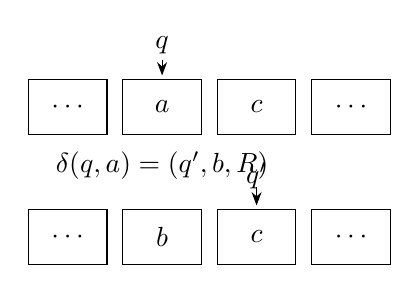
\begin{tikzpicture}[cell/.style={draw,minimum width=10mm,minimum height=7mm},>=Stealth]
\node[cell] at (-1.2,0) {$\cdots$};
\node[cell] at (0,0) {$a$};
\node[cell] at (1.2,0) {$c$};
\node[cell] at (2.4,0) {$\cdots$};
\node at (0,0.78) {$q$};
\draw[->] (0,0.6)--(0,0.4);
\node at (0,-0.75) {$\delta(q,a)=(q',b,R)$};
\node[cell] at (-1.2,-1.65) {$\cdots$};
\node[cell] at (0,-1.65) {$b$};
\node[cell] at (1.2,-1.65) {$c$};
\node[cell] at (2.4,-1.65) {$\cdots$};
\node at (1.2,-0.88) {$q'$};
\draw[->] (1.2,-1.02)--(1.2,-1.25);
\end{tikzpicture}
\caption{一次转移：写入 $b$ 后向右移动，状态由 $q$ 变为 $q'$。}\label{fig:tm-step}
\end{figure}

\paragraph{从一步转移到完整运行}
\begin{definition}[配置与运行]\index{peizhi@配置（图灵机）|hyperpage}\index{yunxing@运行（图灵机）|hyperpage}
机器 $M$ 的一个\emph{配置}记录当前状态、带的内容和读写头的位置，可写为三元组
\[
 C=(q,t,i),
\]
其中 $q\in Q$，$i\in\mathbb Z$，而 $t:\mathbb Z\to\Gamma$ 只有有限多个位置取非空白符。输入 $w=a_0\cdots a_{n-1}\in\Sigma^*$ 时，初始配置为
\[
 C_0(M,w)=(q_0,t_w,0),\qquad
 t_w(j)=
 \begin{cases}a_j,&0\leq j<n,\\\sqcup,&\text{其他情形}.
 \end{cases}
\]
若 $\delta(q,t(i))=(q',b,R)$，则下一配置把 $t(i)$ 改为 $b$，并把读写头位置改为 $i+1$；若方向为 $L$，则位置改为 $i-1$。记“一步转移”为 $C\vdash_M C'$，其有限次迭代记为 $C\vdash_M^* C'$。
\end{definition}

在配置的线性简写中，把状态写在读写头正下方；例如 $u q v$ 表示带上依次写有字符串 $u,v$，读写头正在读 $v$ 的第一个符号，当前状态为 $q$，其余位置均为空白。这个简写记录包含全部非空白格和读写头的一个有限窗口；若读写头位于空白格，也须把该格写出。省略两端多余的空白，并固定窗口的起始位置后，它与上面的配置描述相对应。
从初始配置开始不断应用转移函数，得到配置序列
\[
 C_0\vdash_M C_1\vdash_M C_2\vdash_M\cdots.
\]
如果某一步进入接受态或拒绝态，运行在有限步后\emph{停机}；如果一直没有进入这两个状态，运行就是无限的。因而“机器没有接受输入”有两种可能：它明确进入拒绝态，或者它永远运行下去。后者正是判定和识别的区别所在。

\paragraph{识别、判定与通用模拟}
\begin{definition}[识别与判定]\index{keshibieyuyan@可识别语言|hyperpage}\index{turingpandingsuan@图灵机判定|hyperpage}
设 $M$ 是输入字母表为 $\Sigma$ 的图灵机。
\begin{enumerate}[(a)]
\item $M$ 识别语言
\[
 L(M)=\{w\in\Sigma^*:M\text{ 在输入 }w\text{ 上最终进入 }q_{\mathrm{acc}}\}.
\]
也就是说，$w\in L(M)$ 时机器必须接受；$w\notin L(M)$ 时机器可以拒绝，也可以永不停机。
\item 若对每个输入 $w$ 机器都停机，并且 $w\in L(M)$ 当且仅当机器接受 $w$，则称 $M$\emph{判定}语言 $L(M)$。这时机器对每个输入都给出接受或拒绝的答案。
\end{enumerate}
\end{definition}

识别语言也称递归可枚举语言。若机器在停机时把约定的一段连续符号留在输出区，并用固定的分隔方式读出它，就得到一个字符串；在这种输出约定下，图灵机可以计算部分函数 $f:\Sigma^*\rightharpoonup\Gamma^*$。若它在每个输入上都停机，所计算的就是全函数。输出区的具体编码可以改变表示形式，但不改变哪些函数是可计算的。

\begin{example}[用图灵机识别 $\{0^n1^n:n\geq0\}$]
令输入字母表为 $\Sigma=\{0,1\}$，带字母表为
\[
 \Gamma=\{0,1,X,Y,\sqcup\}.
\]
机器反复寻找最左侧尚未标记的 $0$，把它改为 $X$；随后向右寻找一个尚未标记的 $1$，把它改为 $Y$；再退回带的左端，开始下一轮。当所有 $0$ 都标记完后，检查右侧是否只剩 $Y$。

表中 $(b,D,q')$ 表示“写入 $b$、按 $D$ 移动、进入 $q'$”；未列出的状态均为停机状态。
\begin{center}
{\small
\setlength{\tabcolsep}{2.5pt}
\renewcommand{\arraystretch}{1.15}
\begin{tabular}{c|ccccc}
\toprule
 & $0$ & $1$ & $X$ & $Y$ & $\sqcup$\\\midrule
$q_0$ & $(X,R,q_1)$ & $(1,R,q_{\mathrm{rej}})$ & $(X,R,q_0)$ & $(Y,R,q_3)$ & $(\sqcup,R,q_{\mathrm{acc}})$\\
$q_1$ & $(0,R,q_1)$ & $(Y,L,q_2)$ & $(X,R,q_1)$ & $(Y,R,q_1)$ & $(\sqcup,R,q_{\mathrm{rej}})$\\
$q_2$ & $(0,L,q_2)$ & $(1,L,q_2)$ & $(X,L,q_2)$ & $(Y,L,q_2)$ & $(\sqcup,R,q_0)$\\
$q_3$ & $(0,R,q_{\mathrm{rej}})$ & $(1,R,q_{\mathrm{rej}})$ & $(X,R,q_{\mathrm{rej}})$ & $(Y,R,q_3)$ & $(\sqcup,R,q_{\mathrm{acc}})$\\
\bottomrule
\end{tabular}}
\end{center}
例如，输入 $0011$ 的若干关键配置为
\[
 q_0\,0011\sqcup
 \vdash_M Xq_1\,011\sqcup
 \vdash_M^* q_0\,XXYY\sqcup
 \vdash_M^* XXYq_3Y\sqcup
 \vdash_M^* XXYY\sqcup q_{\mathrm{acc}}\sqcup.
\]
每一轮都会同时消去一个未标记的 $0$ 和一个未标记的 $1$；若某一方先用尽，机器进入拒绝态。因此它接受的恰好是 $0$ 与 $1$ 数量相等且次序为“先全是 $0$、后全是 $1$”的字符串。
\end{example}

\begin{remark}[Church--Turing 论题]\index{Church--Turing@Church--Turing 论题|hyperpage}
Church--Turing 论题认为：凡是按照明确有限规则、能够机械执行的有效算法，都可以由某台图灵机实现。这里的“有效算法”是非形式的直观概念，所以这不是图灵机公理中的定理，也不是在同一形式系统内由公理证明的命题；它是把日常的算法概念与形式化的图灵机概念联系起来的解释原则。
\end{remark}

常见的多带图灵机、带有停留动作的图灵机以及非确定型图灵机，都可以由确定型单带图灵机模拟；模拟可能增加运行时间，但不增加可计算语言的范围。因此在讨论“是否存在算法”时，可以选用最方便的图灵机版本，而不必把模型差异误认为可计算性差异。

\begin{definition}[通用图灵机]\index{tongyongtuolingji@通用图灵机|hyperpage}
图灵机的有限状态和转移表本身也是有限字符串，因而可以用一种有效且无歧义的编码记为 $\langle M\rangle$，再把它编码为自然数。存在一台固定的图灵机 $U$，对任意机器 $M$ 和输入 $w$，在输入 $\langle M,w\rangle$ 上模拟 $M$ 在 $w$ 上的运行：
\[
 M\text{ 接受 }w\Longleftrightarrow U\text{ 接受 }\langle M,w\rangle,
\]
并且 $M$ 拒绝或不停机时，$U$ 也分别模拟相同的行为。这样的 $U$ 称为\emph{通用图灵机}。
\end{definition}

通用机说明了“程序”和“数据”可以用同一种有限对象编码：$\langle M\rangle$ 是机器描述，$w$ 是输入，运行记录则是第三种对象。前面的 Gödel 编码正是利用这一原则把语法操作变成自然数上的函数；对停机计算而言，一段已经结束的运行也只是一个可以检查的有限记录。下面的可枚举性和停机问题都在这个固定的图灵机模型下表述。

\section{统一计算记录：可枚举性与不完备性}\index{tingji@停机|hyperpage}\label{sec:enumerability}
图灵机把外部的有效计算形式化后，可以把前面的“有限证明检查”看成一台识别机：它逐一检查候选证明，在找到目标结论时接受。本节先用计算记录统一可枚举性与算术表示，再证明停机不可判定，最后回到最初的问题：有效给出的算术公理能否决定每一个句子？

\paragraph{搜索能够找到什么：可枚举与可判定}

\begin{definition}[可判定与递归可枚举]\index{kepanding@可判定性|hyperpage}\index{digukemeiju@递归可枚举集|hyperpage}
固定自然数与字符串的一种有效编码。设 $A\subseteq\N$。
\begin{enumerate}[(a)]
\item 若存在一台图灵机 $M$，对每个输入 $n$ 都停机，并且当且仅当 $n\in A$ 时进入接受态（否则进入拒绝态），则称 $A$\emph{可判定}。
\item 若存在一台图灵机 $M$，当且仅当 $n\in A$ 时最终进入接受态，则称 $A$\emph{递归可枚举}（recursively enumerable，RE），也称\emph{可识别}或\emph{可计算枚举}。当 $n\notin A$ 时，机器可以进入拒绝态，也可以永不停机。
\end{enumerate}
通过字符串编码，这些定义同样适用于语言 $L\subseteq\Sigma^*$。在 Church--Turing 论题的意义下，前面所说的有效算法正由这类图灵机刻画；因此下面直接使用图灵机来表述可计算性。
\end{definition}

RE 集也可由图灵机枚举：交错模拟所有输入的识别运行，每当某个运行接受便输出其输入。反过来，给定这样的枚举器，要半判定 $n\in A$，只需运行枚举并等待 $n$ 出现。对不属于集合的输入，半判定程序可以永不停机。

\begin{proposition}
$A$ 可判定，当且仅当 $A$ 与 $\N\setminus A$ 均为 RE 集。
\end{proposition}
\begin{proof}
若可判定，原判定机及交换接受、拒绝结果后的机器分别识别两侧。反过来，交错模拟两侧的识别机，等待其中一台接受；拒绝的运行不触发判断。输入恰属于一侧，所以必有且仅有一侧最终接受，据此即可在有限时间内作出判断。
\end{proof}

\paragraph{统一的接口：存在一段有限计算记录}
固定机器与输入的编码。给定 $e,n,d$，可以机械检查 $d$ 是否编码了机器 $e$ 在输入 $n$ 上的一段完整接受运行：首项是正确的初始配置，相邻配置遵守转移表，末项处于接受态。每项检查都受这段有限记录的长度和编码约束，因此这是原始递归关系。记其算术表示式为 $\operatorname{Acc}(e,n,d)$。将末项条件改为任一停机状态，就得到 $\operatorname{HaltTrace}(e,n,d)$。

这一构造把前面的工具归到同一个框架中：
\[
 \text{输入与程序}\longrightarrow\text{有限配置序列}
 \longrightarrow\text{逐步检查}\longrightarrow\text{算术表示}.
\]
有限序列仍由第~\ref{sec:syntax-arithmetic} 节的方法编码。检查的可表示性保证，每份真实记录都有一个 PA 可证明的数码实例；存在量词再把它变成“某次运行成功结束”。

例如，令 $P$ 为逐一检查 PA 证明、在发现目标句子后接受的机器。对每个句子 $\sigma$，有
\[
 \mathrm{PA}\vdash\sigma
 \quad\Longleftrightarrow\quad
 \mathcal N\models\exists d\,
 \operatorname{Acc}(\overline{\langle P\rangle},
 \overline{\ulcorner\sigma\urcorner},d).
\]
因此，同一个运行检查关系便能描述证明搜索；换一个程序编码，又可描述公式检查或代入计算。这是图灵机带来的统一做法。上式是标准模型中的等价；若要声称两个不同编码的谓词在 PA 内也等价，还须在 PA 中验证相应的模拟，不能直接省略这一步。

\begin{definition}[半可表示性]\index{bankebiaoshixing@半可表示性|hyperpage}
集合 $A\subseteq\N$ 在 PA 中\emph{半可表示}，若存在公式 $\alpha(x)$，使对每个自然数 $n$，
\[
 n\in A\quad\Longleftrightarrow\quad\mathrm{PA}\vdash\alpha(\overline n).
\]
\end{definition}

\begin{proposition}[可枚举性与半可表示性]
$A$ 为 RE 集，当且仅当它在 PA 中半可表示。
\end{proposition}
\begin{proof}
若 $A$ 由 $\alpha$ 半可表示，输入 $n$ 后枚举 PA 证明，找到结论为 $\alpha(\overline n)$ 的证明便停机。这恰好在 $n\in A$ 时发生。这里的“枚举”可由一台图灵机实现：它按编码顺序检查所有有限证明，并在找到目标结论时进入接受态。

反过来，设有一台图灵机 $M$，它恰在 $n\in A$ 时停机并接受。直接使用统一的接受记录公式，令 $C(x,d)=\operatorname{Acc}(\overline{\langle M\rangle},x,d)$，并令 $\alpha(x)=\exists d\,C(x,d)$。

若 $n\in A$，取真实的有限接受记录 $d$，可表示性给出 $\mathrm{PA}\vdash C(\overline n,\overline d)$，再用存在引入。若 PA 证明 $\alpha(\overline n)$，由标准模型中的可靠性，存在真实的自然数记录 $d$ 通过检查，所以 $M$ 确实接受并停机，即 $n\in A$。
\end{proof}

\begin{remark}
这里必须保留“PA 可证明”这一条件。若只要求存在任意算术公式 $\alpha$ 使 $n\in A\leftrightarrow\mathcal N\models\alpha(\overline n)$，得到的是\emph{算术可定义性}，不能据此断定 $A$ 为 RE 集。比如下面停机集的补集可由否定停机记录存在性的公式定义，却不是 RE 集。
\end{remark}

\paragraph{不能统一判定的搜索：停机问题}
\begin{definition}[停机集]\index{tingjiji@停机集|hyperpage}
固定机器描述和输入字符串的一种有效配对编码。对不是合法图灵机描述的字符串，约定其不属于停机集。定义
\[
 \mathrm{HALT}=\{\langle M,w\rangle:
   M\text{ 在输入 }w\text{ 上经过有限步后停机}\}.
\]
由于通用图灵机能够逐步模拟 $M$ 的运行，判断一对编码是否属于 $\mathrm{HALT}$ 正是一个统一的停机问题。
\end{definition}

\begin{theorem}[停机问题不可判定]\index{tingjiwenti@停机问题|hyperpage}
停机集 $\mathrm{HALT}$ 不是可判定集；也就是说，不存在一台对所有输入都停机的图灵机 $H$，能够判断编码为 $e$ 的图灵机在输入 $x$ 上是否停机。
\end{theorem}
\begin{proof}
反设这样的机器 $H$ 存在，规定其输出 $1$ 表示停机，输出 $0$ 表示不停机。利用有效的配对编码，构造一台机器 $D$：输入 $x$ 后，先在 $\langle x,x\rangle$ 上模拟 $H$；若 $H$ 输出 $1$，就进入无限循环；若 $H$ 输出 $0$，就立即进入接受态而停机。

令 $d$ 是 $D$ 的编码。若 $H$ 在 $\langle d,d\rangle$ 上输出 $1$，则 $D(d)$ 按定义不停机，与 $H$ 的判断相反；若输出 $0$，则 $D(d)$ 立即停机，同样与 $H$ 的判断相反。两种情况均矛盾。
\end{proof}
停机集是 RE 集：模拟机在输入 $\langle M,w\rangle$ 上运行 $M$；一旦发现 $M$ 进入接受态或拒绝态，模拟机就进入接受态。于是它恰好在 $\langle M,w\rangle\in\mathrm{HALT}$ 时接受。其补集不是 RE 集，否则由前面的命题，停机集便可判定。这个对角论证与 Gödel 句子的构造有共同点：都把某个对象的编码作为它自己的输入，再使结果与假设的统一判断相反。

\paragraph{更简洁的路线：由停机问题推出不完备性}
现在可以不再逐个构造“我不可证明”的句子，而把整个问题化为算法的极限。关键是：一个完备、有效给出的理论允许同时搜索正反两面的证明；如果这种搜索能正确判断停机，它就会与停机不可判定矛盾。下面明确说明“正确”需要什么假设。

\begin{definition}[有界公式与 $\Sigma_1$-可靠性]\index{youjiegongshi@有界公式|hyperpage}\index{Sigma1gongshi@$\Sigma_1$ 公式|hyperpage}\index{Sigma1kekaoxing@$\Sigma_1$-可靠性|hyperpage}
有界量词是 $\exists x\leq t$ 或 $\forall x\leq t$，其中项 $t$ 不含 $x$；它们分别缩写 $\exists x\,(x\leq t\wedge\cdots)$ 与 $\forall x\,(x\leq t\to\cdots)$。全部量词都有界的公式称为\emph{有界公式}。$\Sigma_1$ 句子形如 $\exists\vec x\,\delta(\vec x)$，其中 $\delta$ 是有界公式。若理论 $T$ 所证明的每个 $\Sigma_1$ 句子都在标准模型 $\mathcal N$ 中为真，则称 $T$ \emph{$\Sigma_1$-可靠}。
\end{definition}
有界公式在给定自然数输入后只需有限检查；$\Sigma_1$ 句子则断言存在一组通过这种检查的自然数见证。它可以含有有界的全称量词，但不能在 $\delta$ 中留下无界的全称或存在量词。

有限运行的算术化可以选成这种形式：把记录及所需辅助编码作为存在量词的见证，读取记录、检查转移等条件均限制在编码给出的界内。这是《Logic and Structure》§8.4--8.6 中 $\Sigma_1$ 表达与可表示性的计算内容。因此存在一个 $\Sigma_1$ 公式 $H(z)$，对每个机器与输入的配对编码 $n$，满足
\[
 n\in\mathrm{HALT}\quad\Longleftrightarrow\quad
 \mathcal N\models H(\overline n),
 \qquad
 n\in\mathrm{HALT}\quad\Longrightarrow\quad
 \mathrm{PA}\vdash H(\overline n).
\]
最后一个蕴含来自真实的有限运行记录：把具体见证代入后，PA 能验证每一步，再作存在引入。它不声称 PA 总能证明一个不停机计算确实不停机。

\begin{theorem}[计算途径的不完备性]
设 $T$ 是同一算术语言中包含 PA 的有效公理化理论。若 $T$ 为 $\Sigma_1$-可靠，则 $T$ 不完备，而且其定理集不可判定。
\end{theorem}
\begin{proof}
$\Sigma_1$-可靠性首先保证一致性：不一致理论会证明假的 $\Sigma_1$ 句子，例如 $\exists x\,(x\ne x)$。

对上述停机公式，真实停机给出 PA 证明，因而也给出 $T$ 的证明；反过来，$\Sigma_1$-可靠性保证 $T$ 证明的停机断言确实为真。所以
\[
 n\in\mathrm{HALT}\quad\Longleftrightarrow\quad T\vdash H(\overline n).
\]
若 $T$ 完备，给定 $n$ 后枚举 $T$ 的有限证明，同时寻找结论为 $H(\overline n)$ 或 $\neg H(\overline n)$ 的证明。有效公理化保证这一搜索可由机器执行，完备性保证必找到一侧，一致性保证不会两侧都找到。找到前者就回答停机；找到后者就回答不停机，因为真实停机本会使 $T$ 证明前者。这便判定了 $\mathrm{HALT}$，矛盾。

即使不假设完备，只要 $T$ 的定理集可判定，也能先有效写出 $H(\overline n)$，再判断它是不是 $T$ 的定理，从而由同一等价式判定停机。因此定理集也不可判定。
\end{proof}

\begin{remark}[两条路线的联系]
这正是《Logic and Structure》定理 8.7.5--8.7.6 所用的计算视角：非可判定的 RE 集经算术表示转化为可证明性问题。对 PA，标准模型满足全部公理，所以它满足这里的可靠性要求。

自指路线具体构造一个不能被决定的句子；计算路线把统一的运行检查、可枚举性和停机不可判定合在一起，简洁地说明为何总有句子无法决定。后一证明用到了 $\Sigma_1$-可靠性，不能只把它改写为一致性。若只假设一致性，仍应使用前面的 Gödel--Rosser 定理或进一步的计算论工具。图灵机统一了论证的组织方式，并没有取消算术表示或理论假设。
\end{remark}

\chapter{集合论}
\begin{wenxintishi}
第一章从集合、函数和基数出发，讨论集合之间的大小关系。本章进一步追问：哪些对象可以称为集合？哪些集合的存在能够由公理保证？通过限制集合的构造方式，公理化集合论（axiomatic set theory）为数学对象提供统一的基础。
\end{wenxintishi}
第一章中的集合论采用较为直观的语言；这里则使用一阶语言把集合及其属于关系形式化。两章讨论的是同一基础对象的不同层次：前者发展大小和结构的直觉，后者说明这些直觉在 ZFC 公理下如何获得严格表达。
\index{gonglijihe lun@公理化集合论|hyperpage}

\section{从朴素集合到 ZFC}
朴素集合论允许直接描述集合，但不能无条件地把每个性质的全部满足者都看成集合。若存在 $R=\{x:x\notin x\}$，代入 $R$ 自身就会得到
\[
 R\in R\quad\Longleftrightarrow\quad R\notin R,
\]
这就是\emph{Russell 悖论}\index{Russell@Russell 悖论|hyperpage}。公理集合论通过明确的存在公理限制哪些集合能够构造。

集合论使用带等号的一阶语言 $\{\in\}$，其中 $\in$ 是二元谓词符号，量词遍历集合。$\varnothing,\{x,y\},\bigcup x,\Pow(x)$ 等不是原始符号，而是在相应存在性及唯一性得到保证后使用的缩写。$x\subseteq y$ 缩写为 $\forall z\,(z\in x\to z\in y)$。

\begin{axiom}[ZFC 公理]\index{ZFC@ZFC 公理|hyperpage}
ZFC（Zermelo--Fraenkel 集合论加选择公理）可用以下九组公理表述。模式中的公式允许有额外参数，均对参数取全称闭包，并避免新引入的集合变量在定义条件中自由出现。
\begin{enumerate}[(1)]
\item \emph{外延公理}：集合由其元素确定。
\[
 \forall x\,\forall y\,
 \bigl(\forall z\,(z\in x\leftrightarrow z\in y)\to x=y\bigr).
\]
\item \emph{分离公理模式}：从已有集合中按公式筛选元素。
\[
 \forall a\,\exists b\,\forall x\,
 \bigl(x\in b\leftrightarrow(x\in a\wedge\varphi(x,\vec p))\bigr).
\]
取恒假的条件便得到空集；外延公理保证其唯一性。
\item \emph{配对公理}：任意两个集合组成一个集合。
\[
 \forall x\,\forall y\,\exists a\,\forall z\,
 (z\in a\leftrightarrow(z=x\vee z=y)).
\]
\item \emph{并集公理}：一个集合中所有元素的元素可以合并成集合。
\[
 \forall a\,\exists b\,\forall x\,
 (x\in b\leftrightarrow\exists y\,(y\in a\wedge x\in y)).
\]
\item \emph{幂集公理}：一个集合的全部子集组成集合。
\[
 \forall a\,\exists b\,\forall x\,(x\in b\leftrightarrow x\subseteq a).
\]
\item \emph{无穷公理}：存在包含空集且对后继操作封闭的集合。
\[
 \exists I\,(\varnothing\in I\wedge
 \forall x\,(x\in I\to x\cup\{x\}\in I)).
\]
\item \emph{替代公理模式}：由公式定义的单值对应将集合映为集合。
\[
 \begin{aligned}
 \forall a\,\bigl[\forall x\in a\,\exists!y\,\varphi(x,y,\vec p)
 \ \to\ \exists b\,\forall y\,(&y\in b\leftrightarrow\\
 &\exists x\in a\,\varphi(x,y,\vec p))\bigr].
 \end{aligned}
\]
\item \emph{正则公理（基础公理）}：每个非空集合都有一个与自身不相交的元素。
\[
 \forall a\,(a\ne\varnothing\to\exists x\in a\,(x\cap a=\varnothing)).
\]
\item \emph{选择公理}：若 $a$ 的每个元素均非空，则存在定义域为 $a$ 的函数 $f$，对每个 $x\in a$ 都满足 $f(x)\in x$。
\end{enumerate}
\end{axiom}
这里 $\forall x\in a$、$\exists x\in a$ 分别表示带条件的全称量词和存在量词；$\exists!$ 表示存在唯一。函数可以用有序对的集合定义，有序对又可定义为 $\langle x,y\rangle=\{\{x\},\{x,y\}\}$，因此选择公理也能完全写成 $\{\in\}$ 语言的一阶句子。分离与替代各自是无限多个句子的模式，而不是一个直接量化所有性质的二阶公理。

\begin{remark}[分离与替代的作用]
分离只能从给定集合中取子集，替代则把给定集合的元素按一个单值关系送到别处，收集所得像。无穷公理给出的 $I$ 不必正好是自然数集；在一个这样的归纳集中取所有归纳子集的交，得到最小归纳集 $\omega$。令 $0=\varnothing$、$S(x)=x\cup\{x\}$，便得到自然数的集合论表示。
\end{remark}

\begin{proposition}[不存在全体集合的集合]
ZFC 中不存在一个包含所有集合为元素的集合。
\end{proposition}
\begin{proof}
若这样的集合 $U$ 存在，分离模式给出 $R=\{x\in U:x\notin x\}$。由于 $R$ 也是集合，有 $R\in U$，于是 $R\in R\leftrightarrow R\notin R$，矛盾。对一般的给定集合 $a$，分离只给出 $\{x\in a:x\notin x\}$；并没有保证这个新集合本身属于 $a$，所以不会自动产生上述矛盾。
\end{proof}

\begin{remark}[在集合论中编码语法]
有限字符串、语法树和有限推导本身都可以表示为集合。项集可刻画为包含变量和常元、并对函数应用封闭的最小集合；公式集类似；“$d$ 是从公理到 $\sigma$ 的有限推导”则是关于这些有限对象的一个可定义关系。这样，集合论也能在内部表达某句子是否有形式证明。

ZFC 的公理模式可以有效枚举，并且在 $\omega$ 上能够解释算术及其语法编码，所以对角构造也适用。准确的结论是：若 ZFC 一致，则它不完备；这里仅用一致性的版本使用 Gödel--Rosser 加强形式。对通常的 Gödel 句子沿用前面的证明时，排除其否定还需相应的 $\omega$-一致性或算术可靠性条件。不能只凭“能够表达自身语法”就省去有效公理化、算术表达能力和一致性这些前提。这也不是 ZFC 对自身一致性的证明。
\end{remark}

\paragraph{公理的典型应用}
下面从具体构造入手，练习如何用公理保证一个对象确实是集合，以及如何利用公理排除不可能的情形。有序对、幂集与归纳原理的题目参考 Jech《Set Theory》第 1 章正文及习题 1.1、1.2、1.9；最后一题对应习题 1.14。以下论证均不需要选择公理。

\begin{example}[有序对、笛卡尔积与函数集]\index{Kuratowski@Kuratowski 有序对|hyperpage}
采用 Kuratowski 定义
\[
 \langle a,b\rangle:=\{\{a\},\{a,b\}\}.
\]
\begin{enumerate}[(a)]
\item 证明 $\langle a,b\rangle=\langle c,d\rangle$ 当且仅当 $a=c$ 且 $b=d$，并注意 $a=b$ 时也应成立。
\item 对集合 $A,B$，用公理构造全部有序对组成的集合 $A\times B$。
\item 说明全部函数 $f:A\to B$ 也组成一个集合，记为 $B^A$。
\end{enumerate}
\end{example}
\begin{proof}
\par\smallskip\noindent\textbf{(a)}\quad 配对公理保证定义中的单元素集、二元素集以及外层集合存在。对非空集合族 $C$，交集可从其中一个成员中用分离构造；因此
\[
 \bigcap\langle a,b\rangle=\{a\},\qquad
 \bigcup\langle a,b\rangle=\{a,b\}.
\]
若两个有序对相等，先取交集得 $\{a\}=\{c\}$，故 $a=c$；再取并集得 $\{a,b\}=\{a,d\}$。若 $b=a$，右侧也只能含 $a$，故 $d=a=b$；若 $b\ne a$，则 $b$ 属于右侧且不等于 $a$，只能有 $b=d$。反向由定义立即得到。

\par\smallskip\noindent\textbf{(b)}\quad 由配对及并集公理，$U=A\cup B=\bigcup\{A,B\}$ 是集合。若 $a\in A,b\in B$，则 $\{a\},\{a,b\}\in\Pow(U)$，从而 $\langle a,b\rangle\in\Pow(\Pow(U))$。两次使用幂集公理，再使用分离，得到
\[
 A\times B=
 \{z\in\Pow(\Pow(U)):\exists a\in A\,\exists b\in B\,
 z=\langle a,b\rangle\}.
\]
这里先找到了一个包含所有候选有序对的集合，再筛出所需对象。

\par\smallskip\noindent\textbf{(c)}\quad 函数以其图像表示，是 $A\times B$ 的子集。于是由幂集和分离，
\[
 B^A=\{f\in\Pow(A\times B):
       \forall a\in A\,\exists!b\in B\,\langle a,b\rangle\in f\}
\]
是集合。这里的存在唯一条件要求每个输入恰有一个输出；并没有断言 $B^A$ 一定非空。例如 $A\ne\varnothing$、$B=\varnothing$ 时，它就是空集。
\end{proof}

\begin{example}[幂集不能包含于原集合]
证明：不存在集合 $X$ 使 $\Pow(X)\subseteq X$。尝试直接使用分离公理，而不诉诸基数比较。
\end{example}
\begin{proof}
反设 $\Pow(X)\subseteq X$。由分离构造
\[
 R=\{x\in X:x\notin x\}.
\]
因 $R\subseteq X$，有 $R\in\Pow(X)$，假设进一步给出 $R\in X$。现在才可以把 $R$ 代入其定义，得到
\[
 R\in R\ \Longleftrightarrow\ (R\in X\wedge R\notin R)
 \ \Longleftrightarrow\ R\notin R,
\]
矛盾。关键不是分离构造有问题，而是假设 $\Pow(X)\subseteq X$ 强迫 $R$ 落回了 $X$。这个论证不需要正则公理。
\end{proof}

\begin{example}[正则公理排除属于关系的有限循环]
\begin{enumerate}[(a)]
\item 证明不存在集合 $x$ 满足 $x\in x$。
\item 更一般地，对任意正整数 $n$，证明不存在
\[
 x_0\in x_1\in\cdots\in x_{n-1}\in x_0.
\]
这里不要求各 $x_i$ 互不相同。
\end{enumerate}
\end{example}
\begin{proof}
\par\smallskip\noindent\textbf{(a)}\quad 若 $x\in x$，对非空集合 $\{x\}$ 使用正则公理。它唯一的元素是 $x$，但 $x\in x\cap\{x\}$，与要求存在交集为空的元素矛盾。

\par\smallskip\noindent\textbf{(b)}\quad 由有限次配对和并集构造 $C=\{x_0,\ldots,x_{n-1}\}$。它非空，正则公理给出 $x_i\in C$ 使 $x_i\cap C=\varnothing$。可是循环中 $x_i$ 的前一个成员既属于 $x_i$，又属于 $C$；当 $i=0$ 时，这个成员取 $x_{n-1}$。故交集不空，矛盾。
\end{proof}

\begin{example}[最小归纳集与数学归纳原理]\index{guinaji@归纳集|hyperpage}
称集合 $I$ 为\emph{归纳集}，若 $\varnothing\in I$，且 $x\in I$ 蕴含 $S(x)=x\cup\{x\}\in I$。无穷公理保证这样的集合存在。
\begin{enumerate}[(a)]
\item 从一个归纳集 $I$ 出发，构造包含于每个归纳集的集合 $\omega$，并说明其定义不依赖于最初选取的 $I$。
\item 若 $A\subseteq\omega$，$\varnothing\in A$ 且 $n\in A\Rightarrow S(n)\in A$，证明 $A=\omega$。
\end{enumerate}
\end{example}
\begin{proof}
\par\smallskip\noindent\textbf{(a)}\quad 不能未经说明就把“全部归纳集”当作一个集合。先在 $\Pow(I)$ 中用分离得到
\[
 \mathcal I=\{J\in\Pow(I):J\text{ 是归纳集}\}.
\]
因为 $I\in\mathcal I$，这是一族非空的集合。再在 $I$ 中用分离定义
\[
 \omega=\{x\in I:\forall J\in\mathcal I\;(x\in J)\}.
\]
每个 $J\in\mathcal I$ 都含空集，所以 $\varnothing\in\omega$。若 $x\in\omega$，则 $x$ 属于每个这样的 $J$，故 $S(x)$ 也属于每个 $J$，从而 $S(x)\in\omega$。于是 $\omega$ 本身归纳。

对任意归纳集 $K$，分离给出 $I\cap K$；它仍归纳，且包含于 $I$，所以 $I\cap K\in\mathcal I$。由定义，$\omega\subseteq I\cap K\subseteq K$。这说明 $\omega$ 包含于\emph{任意}归纳集，不仅是 $I$ 的归纳子集。若从另一个起点得到 $\omega'$，则两者都归纳，最小性给出互相包含，再由外延公理得到 $\omega=\omega'$。

\par\smallskip\noindent\textbf{(b)}\quad 题设恰好说明 $A$ 是归纳集，故最小性给出 $\omega\subseteq A$；结合 $A\subseteq\omega$ 得到相等。对于含参数的公式 $\varphi(n,\vec p)$，先用分离形成
\[
 A=\{n\in\omega:\varphi(n,\vec p)\}.
\]
若证明了 $\varphi(\varnothing,\vec p)$ 及对每个 $n\in\omega$ 的归纳步骤，便可应用上述结论，得到 $\forall n\in\omega\,\varphi(n,\vec p)$。这说明算术中的归纳原理如何来自最小归纳集的性质。
\end{proof}

\begin{example}[从替代推出分离]
在空集已经存在的前提下，用本节陈述的替代公理模式证明：对任意集合 $A$ 和公式 $\varphi(x,\vec p)$，满足 $\varphi$ 的那些 $A$ 中元素组成集合。证明中不要预先使用分离。
\end{example}
\begin{proof}
若没有 $x\in A$ 满足 $\varphi(x,\vec p)$，空集就是所需集合。

否则取一个 $a\in A$ 满足 $\varphi(a,\vec p)$。考虑公式
\[
 \psi(x,y):=
 (\varphi(x,\vec p)\wedge y=x)
 \vee(\neg\varphi(x,\vec p)\wedge y=a).
\]
对每个 $x\in A$，存在唯一的 $y$ 满足 $\psi(x,y)$：符合条件的元素映到自身，其余元素统一映到 $a$。由替代，其像
\[
 B=\{y:\exists x\in A\,\psi(x,y)\}
\]
是集合。

若 $y\in B$，则 $y$ 或者等于一个满足 $\varphi$ 的 $x\in A$，或者等于事先选定的 $a$；两种情形都给出 $y\in A$ 且 $\varphi(y,\vec p)$。反之，若 $y\in A$ 且 $\varphi(y,\vec p)$，取输入 $x=y$ 就有 $\psi(x,y)$，故 $y\in B$。所以
\[
 y\in B\quad\Longleftrightarrow\quad y\in A\wedge\varphi(y,\vec p),
\]
这正是分离所要求的集合。证明中只选取一个已经由存在条件给出的元素 $a$，不需要选择公理。
\end{proof}
\begin{remark}[替代模式的两种表述]
Jech 习题 1.14 使用允许部分定义的单值关系，直接对 $\varphi(x,\vec p)\wedge y=x$ 应用替代即可。本节的替代模式要求每个输入都恰有一个输出，所以先用上面的分情况定义把对应补成全定义。空集的存在是此题明确保留的前提，不能在声称推出分离时又用分离制造空集。
\end{remark}

\chapter{初等数论}
\begin{wenxintishi}
辗转相除法把整除问题化为逐步缩小的计算，Bézout 等式由此连接素因子分解与同余运算。中国剩余定理把多个模数下的信息合并起来；最后，同样的相减过程又出现在有理数的二叉搜索中。
\end{wenxintishi}
本章中 $\N=\{0,1,2,\ldots\}$，正整数集记为 $\N_{>0}$，整数集记为 $\mathbb Z$。

\section{整除、辗转相除与素因子分解}
\begin{definition}[整除]\index{zhengchu@整除|hyperpage}
设 $a,b\in\mathbb Z$。若存在 $c\in\mathbb Z$ 使 $b=ac$，则称 $a$\emph{整除} $b$，记为 $a\mid b$；否则记为 $a\nmid b$。
\end{definition}
整除关系具有自反性和传递性。在整数上，$a\mid b$ 且 $b\mid a$ 只能推出 $a=\pm b$；限制到自然数后，便得到反对称性，因此 $(\N,\mid)$ 是偏序集。注意这里的顺序不是通常的大小顺序：$1$ 整除每个自然数，而每个自然数都整除 $0$；$2$ 与 $3$ 则不可比较。

\begin{definition}[最大公因数与最小公倍数]
对不全为零的整数 $a,b$，定义\index{zuidagongyinshu@最大公因数|hyperpage}
\[
 \gcd(a,b)=\max\{d\in\N_{>0}:d\mid a,\ d\mid b\},
\]
并约定 $\gcd(0,0)=0$。若 $ab\ne0$，定义\index{zuixiaogongbeishu@最小公倍数|hyperpage}
\[
 \operatorname{lcm}(a,b)=\min\{c\in\N_{>0}:a\mid c,\ b\mid c\};
\]
若 $ab=0$，约定 $\operatorname{lcm}(a,b)=0$。
\end{definition}
上述最大值与最小值按通常的数值大小取得。它们确实存在：非零整数的正因数有限，而 $|ab|$ 是两个非零整数的正公倍数。至于 $\gcd(a,b)$ 是否被\emph{每个公因数整除}，还需要证明；“数值最大”本身并不自动给出这个结论。

\paragraph{从带余除法得到 Bézout 等式}
设 $0<a\le b$。带余除法给出唯一的 $q,r\in\N$，使
\[
 b=aq+r,\qquad 0\le r<a.
\]
因为 $r=b-aq$ 且 $b=aq+r$，$a,b$ 的公因数恰好是 $r,a$ 的公因数。因此
$\gcd(a,b)=\gcd(r,a)$。反复进行这一步，较小的数严格下降，最终必到达余数为零的情形。这就是\emph{辗转相除法}（Euclidean algorithm）\index{zhanzhuanxiangchufa@辗转相除法|hyperpage}。

不仅可以算出最大公因数，还可以同时保留它如何由输入线性组合得到。
\begin{theorem}[扩展 Euclid 算法与 Bézout 等式]\label{thm:bezout}
\index{Bezout@Bézout 等式|hyperpage}\index{kuozhanEuclidsuanfa@扩展 Euclid 算法|hyperpage}
对任意整数 $a,b$，存在 $u,v\in\mathbb Z$ 使
\[
 \gcd(a,b)=au+bv.
\]
当 $0\le a\le b$ 时，下面的递归算法返回 $(d,u,v)$，其中 $d=\gcd(a,b)=au+bv$：
\begin{enumerate}[(a)]
\item 若 $a=0$，返回 $(b,0,1)$。
\item 若 $a>0$，写 $b=aq+r$，$0\le r<a$，递归计算输入 $(r,a)$，得到 $(d,m,n)$，再返回 $(d,n-qm,m)$。
\end{enumerate}
\end{theorem}
\begin{proof}
每次递归的第一个输入严格下降，所以算法终止。对第一个输入作强归纳：$a=0$ 时结论显然；$a>0$ 时，由归纳假设，递归返回值满足
\[
 d=\gcd(r,a)=rm+an.
\]
公因数集合不变，故 $d=\gcd(a,b)$；代入 $r=b-aq$，得到
\[
 d=(b-aq)m+an=a(n-qm)+bm,
\]
正好是算法返回的系数。一般整数输入先取绝对值并按大小排序，再相应调整系数的符号与位置；两个输入均为零时取 $u=v=0$ 即可。
\end{proof}

\begin{example}
用扩展 Euclid 算法计算 $\gcd(30,84)$，并将它写为 $30,84$ 的整数线性组合。
\end{example}
\begin{proof}
先逐次求余：
\[
 84=2\cdot30+24,\qquad30=24+6,\qquad24=4\cdot6.
\]
因此最大公因数为 $6$。逆向代入给出
\[
 6=30-24=30-(84-2\cdot30)=3\cdot30-84.
\]
\end{proof}

\begin{corollary}[最大公因数的两种刻画]\label{cor:gcd-characterization}
若 $a,b$ 不全为零，则
\[
 \gcd(a,b)=\min\{au+bv:u,v\in\mathbb Z,\ au+bv>0\}.
\]
此外，对任意整数 $c$，
\[
 c\mid a\ \text{且}\ c\mid b\quad\Longleftrightarrow\quad c\mid\gcd(a,b).
\]
后一等价式对 $a=b=0$ 也成立。
\end{corollary}
\begin{proof}
令 $d=\gcd(a,b)>0$。由于 $d\mid a,b$，每个正线性组合都为 $d$ 的正倍数，因而至少为 $d$；Bézout 等式又说明 $d$ 本身就是这样的线性组合，所以它是最小者。若 $c\mid a,b$，则 $c$ 整除 Bézout 等式右端，故 $c\mid d$；反方向由 $d\mid a,b$ 和传递性得到。两个输入均为零时，等价式两边都对所有整数 $c$ 成立。
\end{proof}
这也说明最大公因数是整除偏序中的最大下界，而不只是数值最大的公因数。

\begin{definition}[互素与素数]
\index{husu@互素|hyperpage}\index{sushu@素数|hyperpage}
若 $\gcd(a,b)=1$，称整数 $a,b$ \emph{互素}。整数 $p>1$ 称为\emph{素数}，若其正因数只有 $1,p$。大于 $1$ 且不是素数的整数称为\emph{合数}。
\end{definition}
由 Bézout 等式，$a,b$ 互素当且仅当存在整数 $u,v$ 使 $au+bv=1$。

\begin{lemma}[互素的乘积性质与 Euclid 引理]\label{lem:euclid-prime}
\index{Euclidyinli@Euclid 引理|hyperpage}
\begin{enumerate}[(a)]
\item 若 $a$ 分别与 $b,c$ 互素，则 $a$ 与 $bc$ 互素。
\item 若 $\gcd(a,b)=1$ 且 $a\mid bc$，则 $a\mid c$。特别地，若素数 $p$ 整除 $bc$，则 $p\mid b$ 或 $p\mid c$。
\end{enumerate}
\end{lemma}
\begin{proof}
\par\smallskip\noindent\textbf{(a)}\quad 写 $au+bv=1$、$au'+cv'=1$。相乘并整理得
\[
 a(auu'+ucv'+u'bv)+bcvv'=1,
\]
故 $a$ 与 $bc$ 互素。

\par\smallskip\noindent\textbf{(b)}\quad 将 $au+bv=1$ 乘以 $c$，得到 $c=auc+bvc$，右端两项都被 $a$ 整除。若 $p\nmid b$，由素数的定义 $\gcd(p,b)=1$，于是前一结论给出 $p\mid c$。
\end{proof}

\begin{theorem}[算术基本定理]\index{suanshujibendingli@算术基本定理|hyperpage}
每个正整数都可唯一地写为按非降顺序排列的素数乘积；$1$ 对应空乘积。等价地，每个 $n>1$ 唯一地写成
\[
 n=p_1^{\alpha_1}\cdots p_k^{\alpha_k},\qquad
 p_1<\cdots<p_k,\quad\alpha_i\in\N_{>0}.
\]
\end{theorem}
\begin{proof}
存在性对 $n$ 作强归纳。$n=1$ 时取空乘积；若 $n>1$ 为素数，无须分解；否则 $n=ab$，其中 $1<a,b<n$，把 $a,b$ 的素数分解合并即可。

若唯一性不成立，取具有两个不同非降素数分解的最小正整数 $n$，写成
\[
 n=p_1\cdots p_r=q_1\cdots q_s.
\]
由 Euclid 引理反复应用，$p_1$ 整除某个 $q_j$，而 $q_j$ 为素数，所以 $p_1=q_j$。从两边各消去这一个因子，就得到小于 $n$ 的正整数的两种分解。由最小性，它们的素因子及重数相同；再添回所消去的因子，原来的两种分解也相同，矛盾。
\end{proof}

\begin{corollary}
设 $a,b>0$，将二者涉及的素数统一列为 $p_1,\ldots,p_k$，允许指数为零，写
$a=\prod_i p_i^{\alpha_i}$、$b=\prod_i p_i^{\beta_i}$。则
\[
 \gcd(a,b)=\prod_i p_i^{\min(\alpha_i,\beta_i)},\qquad
 \operatorname{lcm}(a,b)=\prod_i p_i^{\max(\alpha_i,\beta_i)}.
\]
从而 $\gcd(a,b)\operatorname{lcm}(a,b)=ab$，且每个公倍数都被最小公倍数整除。
\end{corollary}
\begin{proof}
由素因子分解的唯一性，整除等价于每个素因子的指数逐项不大于另一方的指数。因此公因数的指数上界是最小值，公倍数的指数下界是最大值。乘积公式来自 $\min(\alpha,\beta)+\max(\alpha,\beta)=\alpha+\beta$；零公倍数也被最小公倍数整除。
\end{proof}

整除关系可以用图直观表示。下面只画 $30$ 的正因数，线段向上表示整除，并省去可由传递性得到的连线。例如 $6$ 与 $10$ 的最大公因数为 $2$，最小公倍数为 $30$。
\begin{center}
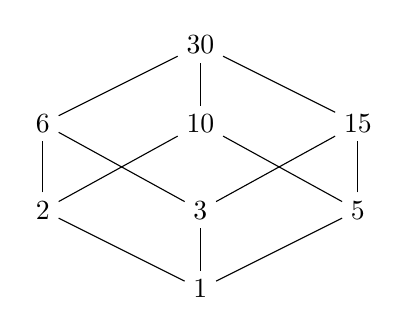
\begin{tikzpicture}[every node/.style={fill=white,inner sep=3pt}]
\node (one) at (0,0) {$1$};
\node (two) at (-2,1) {$2$};\node (three) at (0,1) {$3$};\node (five) at (2,1) {$5$};
\node (six) at (-2,2.1) {$6$};\node (ten) at (0,2.1) {$10$};\node (fifteen) at (2,2.1) {$15$};
\node (thirty) at (0,3.1) {$30$};
\draw (one)--(two);\draw (one)--(three);\draw (one)--(five);
\draw (two)--(six);\draw (two)--(ten);\draw (three)--(six);\draw (three)--(fifteen);
\draw (five)--(ten);\draw (five)--(fifteen);
\draw (six)--(thirty);\draw (ten)--(thirty);\draw (fifteen)--(thirty);
\end{tikzpicture}
\end{center}

\section{同余、Euler 函数与中国剩余定理}
\begin{definition}[同余与剩余类]\index{tongyu@同余|hyperpage}\index{shengyulei@剩余类|hyperpage}
固定正整数 $m$。若 $m\mid(a-b)$，则称 $a,b$ \emph{模 $m$ 同余}，记为 $a\equiv b\pmod m$。这是整数上的等价关系。$a$ 的剩余类为
\[
 \overline a=\{a+km:k\in\mathbb Z\},
\]
所有剩余类组成的集合记为 $\mathbb Z_m=\mathbb Z/m\mathbb Z$。带余除法说明
$\mathbb Z_m=\{\overline0,\ldots,\overline{m-1}\}$。
\end{definition}
本节的横线表示模某个整数的剩余类，与第三章表示自然数的数码闭项的记号用途不同；模数由上下文指定。

若 $a\equiv a'\pmod m$ 且 $b\equiv b'\pmod m$，则
\[
 a+b\equiv a'+b'\pmod m,\qquad ab\equiv a'b'\pmod m.
\]
前者由差相加得到；后者由 $ab-a'b'=a(b-b')+b'(a-a')$ 得到。因此可以定义
$\overline a+\overline b=\overline{a+b}$、$\overline a\,\overline b=\overline{ab}$，不依赖代表元的选择。

\begin{proposition}[模逆元与消去律]\index{moniyuan@模逆元|hyperpage}
$\overline c\in\mathbb Z_m$ 存在乘法逆元，当且仅当 $\gcd(c,m)=1$。在此条件下，
\[
 ac\equiv bc\pmod m\quad\Longrightarrow\quad a\equiv b\pmod m.
\]
\end{proposition}
\begin{proof}
若 $cu+mv=1$，则 $cu\equiv1\pmod m$，故 $\overline u$ 是逆元。反之，若 $cu\equiv1\pmod m$，则存在整数 $v$ 使 $cu+mv=1$，所以 $c,m$ 互素。消去律只需将原同余式两边乘以 $u$。
\end{proof}
不能任意约去同余式中的公因子。例如 $2\cdot1\equiv2\cdot4\pmod6$，但 $1\not\equiv4\pmod6$。

\begin{definition}[单位与 Euler 函数]
\index{danweiqun@单位群|hyperpage}\index{Eulerhanshu@Euler 函数|hyperpage}
模 $m$ 的可逆剩余类称为\emph{单位}，其集合为
\[
 \mathbb Z_m^\times=\{\overline a:\gcd(a,m)=1\}.
\]
它对乘法封闭，含单位元，每个元素有逆元，乘法又满足结合律，因此构成一个群，称为\emph{单位群}。定义
\[
 \varphi(m)=|\mathbb Z_m^\times|
 =|\{a:1\le a\le m,\ \gcd(a,m)=1\}|.
\]
特别地，$\varphi(1)=1$；此时唯一剩余类满足 $\overline0=\overline1$。
\end{definition}

\begin{theorem}[Fermat 小定理与 Euler 定理]
\index{Fermatxiaodingli@Fermat 小定理|hyperpage}\index{Eulerdingli@Euler 定理|hyperpage}
\begin{enumerate}[(a)]
\item 若 $p$ 为素数，则对每个整数 $a$，$a^p\equiv a\pmod p$；若 $p\nmid a$，则 $a^{p-1}\equiv1\pmod p$。
\item 若 $m\ge1$ 且 $\gcd(a,m)=1$，则 $a^{\varphi(m)}\equiv1\pmod m$。
\end{enumerate}
\end{theorem}
\begin{proof}
\par\smallskip\noindent\textbf{(a)}\quad 若 $p\nmid a$，乘以 $a$ 将模 $p$ 的非零剩余类置换：乘积仍非零，且由消去律不同的类不会变成同一个类。于是
\[
 a^{p-1}(p-1)!\equiv(p-1)!\pmod p.
\]
每个 $1,\ldots,p-1$ 都与 $p$ 互素，它们的乘积也与 $p$ 互素，故可消去阶乘，得到 $a^{p-1}\equiv1$。两边乘以 $a$ 得 $a^p\equiv a$；若 $p\mid a$，后一同余式两边均为零。

\par\smallskip\noindent\textbf{(b)}\quad 将单位列为 $\overline{u_1},\ldots,\overline{u_{\varphi(m)}}$。由于 $\overline a$ 可逆，映射 $\overline u\mapsto\overline a\,\overline u$ 是单位集合上的双射。因此
\[
 a^{\varphi(m)}\prod_{i=1}^{\varphi(m)}u_i
 \equiv\prod_{i=1}^{\varphi(m)}u_i\pmod m.
\]
右侧乘积也是单位，可以消去，结论随之成立。
\end{proof}

\begin{proposition}[按最大公因数计数]
对每个正整数 $m$，都有
\[
 \sum_{d\mid m,\ d>0}\varphi(d)=m.
\]
\end{proposition}
\begin{proof}
记 $\overline i_r$ 为整数 $i$ 模 $r$ 的剩余类。按 $\gcd(i,m)$ 的值，将 $\mathbb Z_m$ 写成不交并：
\[
\begin{aligned}
 \mathbb Z_m
 &=\bigsqcup_{d\mid m}
   \{\overline i_m\in\mathbb Z_m:\gcd(i,m)=d\}\\
 &=\bigsqcup_{d\mid m}
   \{\overline{di}_m:\overline i_{m/d}\in\mathbb Z_{m/d},\
                        \gcd(di,m)=d\}\\
 &\simeq\bigsqcup_{d\mid m}
   \{\overline i_{m/d}\in\mathbb Z_{m/d}:\gcd(i,m/d)=1\}\\
 &=\bigsqcup_{d\mid m}\mathbb Z_{m/d}^{\times}.
\end{aligned}
\]
这里 $d$ 遍历 $m$ 的正因数，$\bigsqcup$ 表示不交并，$\simeq$ 表示双射。第三行对每个固定的 $d$ 使用对应
\[
 \overline{di}_m\longleftrightarrow\overline i_{m/d}.
\]
它是良定义的双射，因为 $di\equiv dj\pmod m$ 当且仅当 $i\equiv j\pmod{m/d}$；而
$\gcd(di,m)=d$ 当且仅当 $\gcd(i,m/d)=1$。不同 $d$ 的单位集合在不交并中保留各自的分量标记。

于是取基数，得到
\[
 m=|\mathbb Z_m|
 =\sum_{d\mid m}|\mathbb Z_{m/d}^{\times}|
 =\sum_{d\mid m}\varphi\!\left(\frac md\right)
 =\sum_{d\mid m}\varphi(d).
\]
最后一步用到 $d\mapsto m/d$ 是 $m$ 的正因数集合上的双射。
\end{proof}

\begin{example}[循环小数与同余]
解释 $1/7=0.\overline{142857}$ 的循环节为何恰有六位，并说明同余运算如何描述一般进位制下的循环长度。
\end{example}
\begin{proof}
由 $7\cdot142857=10^6-1$，等比级数求和给出上述循环小数。一般地，设整数 $b\ge2,n>1$ 满足 $\gcd(b,n)=1$。以 $b$ 进位制作 $1/n$ 的长除法，第 $k$ 步余数是 $b^k$ 模 $n$ 的余数。乘以 $b$ 是剩余类上的置换，故余数从 $1$ 出发循环；首次回到 $1$ 的步数，即使 $b^k\equiv1\pmod n$ 的最小正整数 $k$，就是最小循环节长度。

Euler 定理保证这样的 $k$ 存在，且 $k\mid\varphi(n)$：写 $\varphi(n)=qk+r$，$0\le r<k$，则 $b^r\equiv1$，由最小性 $r=0$。对 $b=10,n=7$，$\varphi(7)=6$；而
\[
 10\equiv3,\quad10^2\equiv2,\quad10^3\equiv6\pmod7,
\]
排除了 $6$ 的所有真正因数 $1,2,3$，所以最小循环节长度为 $6$。
\end{proof}

\paragraph{将不同模数下的信息合并}
一个整数模 $m_1,\ldots,m_t$ 的余数可以同时记录。模数两两互素时，这些记录恰好确定模其乘积的一个剩余类。
\begin{theorem}[中国剩余定理]\label{thm:crt}
\index{zhongguoshengyudingli@中国剩余定理|hyperpage}
设 $m_1,\ldots,m_t\ge2$ 两两互素，$M=m_1\cdots m_t$。对任意整数 $a_1,\ldots,a_t$，同余方程组
\[
 x\equiv a_i\pmod{m_i}\qquad(1\le i\le t)
\]
在模 $M$ 的意义下有唯一解。等价地，取各个余数的映射
\[
 \pi:\mathbb Z_M\longrightarrow\prod_{i=1}^t\mathbb Z_{m_i},
 \qquad \overline x\longmapsto
 (x\bmod m_1,\ldots,x\bmod m_t)
\]
是双射，并保持加法、乘法。
\end{theorem}
\begin{proof}
令 $M_i=M/m_i$。由模数两两互素及互素的乘积性质，$\gcd(M_i,m_i)=1$，故可取整数 $u_i$ 使 $M_i u_i\equiv1\pmod{m_i}$。令 $e_i=M_i u_i$，则
\[
 e_i\equiv\begin{cases}1&\pmod{m_i},\\0&\pmod{m_j}\quad(j\ne i).\end{cases}
\]
因此 $x=\sum_{i=1}^t a_i e_i$ 满足全部同余式。

若 $x,y$ 都满足，则每个 $m_i$ 都整除 $x-y$。两两互素的整数分别整除同一个数时，它们的乘积也整除该数：对于两个因子，写 $x-y=m_1z$，由 $m_2\mid m_1z$ 及 Euclid 引理得 $m_2\mid z$；再归纳推广到全部因子。因此 $M\mid(x-y)$，给出唯一性。加法、乘法的保持性来自同余与这两种运算相容。
\end{proof}
第三章用余数编码有限序列时，正是利用这个定理同时指定多个余数；这里的 $e_i$ 可以理解为只在第 $i$ 个分量取值为 $1$ 的选择器。

\begin{example}
求解 $x\equiv2\pmod3$、$x\equiv3\pmod5$、$x\equiv2\pmod7$。
\end{example}
\begin{proof}
取 $M=105$，相应 $M_i$ 为 $35,21,15$。它们模 $3,5,7$ 的逆元分别可取 $2,1,1$，故
\[
 x\equiv2\cdot70+3\cdot21+2\cdot15
 =233\equiv23\pmod{105}.
\]
\end{proof}

\begin{proposition}[Euler 函数的乘积公式]
若 $n=p_1^{\alpha_1}\cdots p_k^{\alpha_k}>1$ 是素因子分解，则
\[
 \varphi(n)=\prod_{i=1}^k(p_i^{\alpha_i}-p_i^{\alpha_i-1})
 =n\prod_{i=1}^k\left(1-\frac1{p_i}\right).
\]
特别地，若 $a,b>0$ 互素，则 $\varphi(ab)=\varphi(a)\varphi(b)$。
\end{proposition}
\begin{proof}
模 $p^\alpha$ 的 $p^\alpha$ 个剩余类中，不与模数互素的恰好是 $p$ 的倍数，共 $p^{\alpha-1}$ 个，因此
$\varphi(p^\alpha)=p^\alpha-p^{\alpha-1}$。

中国剩余定理把模 $n$ 的类与模各个 $p_i^{\alpha_i}$ 的类一一对应。一个整数与 $n$ 互素，当且仅当它与每个 $p_i^{\alpha_i}$ 互素，因而该双射限制为单位集合之间的双射。各分量可以独立选择，单位的总数便是各个单位集合大小的乘积。互素的 $a,b$ 没有共同素因子，故乘积公式还给出乘法性；含因子 $1$ 的情形由 $\varphi(1)=1$ 得到。
\end{proof}

\begin{example}[RSA 的算术原理]\index{RSA@RSA 的算术原理|hyperpage}
取不同素数 $p,q$，令 $N=pq$，则 $\varphi(N)=(p-1)(q-1)$。选取正整数 $e$，满足 $\gcd(e,\varphi(N))=1$，再取正整数 $d$ 使
\[
 ed\equiv1\pmod{\varphi(N)}.
\]
公开 $(N,e)$，保留 $d$。对消息 $m\in\mathbb Z_N^\times$，加密得到 $c\equiv m^e\pmod N$，解密时计算 $c^d\pmod N$。证明解密恢复 $m$。
\end{example}
\begin{proof}
写 $ed=1+k\varphi(N)$，其中 $k\ge0$。由 Euler 定理，
\[
 c^d\equiv m^{ed}
 =m\bigl(m^{\varphi(N)}\bigr)^k
 \equiv m\pmod N.
\]
这里模逆元 $d$ 可用扩展 Euclid 算法求得；例如取 $p=5,q=11$，则 $N=55$、$\varphi(N)=40$，可取 $e=3,d=27$。消息 $m=2$ 加密为 $c=8$，解密时 $8^{27}=2^{81}\equiv2\pmod{55}$。
\end{proof}
\begin{remark}
对不同素数的乘积 $N=pq$，上述恢复公式事实上对所有 $m\in\mathbb Z_N$ 成立。模 $p$ 考察：若 $p\mid m$，$m^{ed}\equiv m\equiv0$；否则，由 $p-1\mid ed-1$ 和 Fermat 小定理，仍有 $m^{ed}\equiv m$。模 $q$ 同理，再由中国剩余定理得到模 $N$ 的等式。这里说明的是幂运算可逆的算术机制。
\end{remark}

\section{有理数逼近与 Stern--Brocot 树}
若希望用简单分数逼近一个正实数，可以不断缩小包含它的区间。这里不取通常的算术平均，而将两个端点的分子、分母分别相加。
\begin{definition}[中介分数与 Stern--Brocot 树]
\index{zhongjiefenshu@中介分数|hyperpage}\index{SternBrocot@Stern--Brocot 树|hyperpage}
对非负分数 $a/b<c/d$，其中 $b,d>0$，称
\[
 \frac{a+c}{b+d}
\]
为它们的\emph{中介分数}。从边界 $0/1$ 与形式记号 $1/0=+\infty$ 开始，取中介分数 $1/1$ 为根；对每个区间，将其中介分数作为结点，再递归处理左右两个子区间，由此得到 \emph{Stern--Brocot 树}。边界 $1/0$ 只是记号，不是有理数结点。
\end{definition}
若 $a/b<c/d$，直接通分可得 $a/b<(a+c)/(b+d)<c/d$；右边界为 $1/0$ 时，左侧不等式仍成立，而右侧解释为小于 $+\infty$。树的最初三层如下：
\begin{center}
\begin{tikzpicture}[every node/.style={font=\normalsize},>=Stealth]
\node (a) at (0,0) {$\frac11$};
\node (b) at (-2.7,-1.3) {$\frac12$};
\node (c) at (2.7,-1.3) {$\frac21$};
\node (d) at (-4,-2.6) {$\frac13$};
\node (e) at (-1.4,-2.6) {$\frac23$};
\node (f) at (1.4,-2.6) {$\frac32$};
\node (g) at (4,-2.6) {$\frac31$};
\draw[->] (a)--(b);\draw[->] (a)--(c);
\draw[->] (b)--(d);\draw[->] (b)--(e);
\draw[->] (c)--(f);\draw[->] (c)--(g);
\end{tikzpicture}
\end{center}
要寻找目标 $x>0$，在当前区间比较 $x$ 与中介分数：相等即停止；$x$ 较小就进入左子区间，较大就进入右子区间。这是一种二叉搜索。不过，仅凭每一步缩小区间，还不能断言每个有理数都能在有限步内找到。关键是将搜索转成正整数上的递减过程。

\paragraph{用矩阵记录区间}
把端点 $a/b<c/d$ 记为矩阵
\[
 A=\begin{bmatrix}a&c\\b&d\end{bmatrix}.
\]
向左搜索保留左端点，将右端点换为中介分数；向右则反过来。因此两个操作分别为
\[
 L=\begin{bmatrix}1&1\\0&1\end{bmatrix},\qquad
 R=\begin{bmatrix}1&0\\1&1\end{bmatrix},
\]
\[
 AL=\begin{bmatrix}a&a+c\\b&b+d\end{bmatrix},\qquad
 AR=\begin{bmatrix}a+c&c\\b+d&d\end{bmatrix}.
\]
初始矩阵 $A_0=\begin{bmatrix}0&1\\1&0\end{bmatrix}$ 的行列式为 $-1$，而 $\det L=\det R=1$，所以搜索途中始终有
\[
 ad-bc=-1,\qquad bc-ad=1.
\]
任何公因数若整除 $a+c,b+d$，也整除 $b(a+c)-a(b+d)=bc-ad=1$。所以每个中介分数自动最简，无须另做约分。

\begin{theorem}
每个正有理数都能在 Stern--Brocot 树中找到，即上述搜索在有限步内停止。
\end{theorem}
\begin{proof}
设要寻找的最简正有理数为 $p/q$，当前区间为
\[
 \frac ab<\frac pq<\frac cd.
\]
区间矩阵 $A=\begin{bmatrix}a&c\\b&d\end{bmatrix}$ 的行列式为 $-1$，因此方程组
\[
 \begin{cases}
 am+cn=p,\\
 bm+dn=q
 \end{cases}
\]
有唯一解 $(m,n)$。具体地，
\[
 m=cq-dp,\qquad n=bp-aq.
\]
由端点与 $p/q$ 的严格大小关系，$m,n$ 都是正整数；初始右端点为 $1/0$ 时，也有 $m=q>0$。于是
\[
 \frac pq=\frac{am+cn}{bm+dn}.
\]
若 $m=n$，则
\[
 \frac pq=\frac{a+c}{b+d},
\]
当前中介分数就是要找的数，搜索结束。

否则，先设 $m<n$。将分子、分母中的同一组项合并，得到
\[
 \frac{a+c}{b+d}
 <\frac pq
 =\frac{m(a+c)+(n-m)c}{m(b+d)+(n-m)d}
 <\frac cd.
\]
因此进入右区间，新的端点为 $(a+c)/(b+d)$ 与 $c/d$，目标相对于新端点的系数由 $(m,n)$ 变成 $(m,n-m)$。

若 $m>n$，则同样有
\[
 \frac ab
 <\frac pq
 =\frac{(m-n)a+n(a+c)}{(m-n)b+n(b+d)}
 <\frac{a+c}{b+d}.
\]
此时进入左区间，系数变成 $(m-n,n)$。这些严格不等式可由 $bc-ad=1$ 通分验证；右端点为 $1/0$ 时，最右侧的不等式解释为小于 $+\infty$。

这正是相减形式的 Euclid 算法。每一步的两个系数仍为正整数，而 $m+n$ 严格减小，所以必在有限步内到达 $m=n$，也就找到目标 $p/q$。
\end{proof}
\begin{remark}[搜索与辗转相除]
端点的分子、分母虽然不断增大，目标相对于端点的系数却在执行
$(m,n)\mapsto(m,n-m)$ 或 $(m-n,n)$。将连续向同一方向的多次相减合成一次，就得到带商的辗转相除。这里保证终止的是正整数系数的递减。

此外，每个正有理数只出现一次：结点的所有后代都严格位于对应子区间内部，而左右子区间的内部互不相交。因此它不会在自己的后代或另一个分支中重复出现。
\end{remark}

\begin{example}[逼近黄金比例的倒数]
设 $\alpha=(\sqrt5-1)/2$。用 Stern--Brocot 搜索给出若干有理逼近，并解释分母较小的分数为何受到相邻端点的限制。
\end{example}
\begin{proof}
比较中介分数与 $\alpha\approx0.618034$，依次得到
\[
 \frac11,\quad\frac12,\quad\frac23,\quad\frac35,
 \quad\frac58,\quad\frac8{13},\quad\frac{13}{21},\ldots
\]
例如 $1/2<\alpha<1$，下一次比较 $2/3$ 后保留区间 $(1/2,2/3)$；随后 $3/5<\alpha<2/3$，再得到 $3/5<\alpha<5/8$。相应区间矩阵为
\[
 A_0LRLR=\begin{bmatrix}3&5\\5&8\end{bmatrix}.
\]
这些分数的分子、分母沿着 Fibonacci 数列增长。若 $F_0=0,F_1=1$、$F_{n+2}=F_{n+1}+F_n$，它们是 $F_n/F_{n+1}$。由递推式可验证
\[
 F_n=\frac{\tau^n-(-\alpha)^n}{\sqrt5},\qquad
 \tau=\frac{1+\sqrt5}{2}=\frac1\alpha,
\]
两边具有相同初值并满足同一递推；因 $|\alpha/\tau|<1$，所得比值趋于 $1/\tau=\alpha$。

再看任何相邻端点 $a/b<c/d$，其行列式条件为 $bc-ad=1$。若最简分数 $p/q$ 严格位于两者之间，前面证明中的正整数坐标给出
\[
 q=bm+dn\ge b+d.
\]
这说明区间内部的任何分数，其分母至少是两个端点分母之和。例如 $3/5$ 与 $5/8$ 之间的分数，分母至少为 $13$，而中介分数 $8/13$ 恰好达到这一界。
\end{proof}
\begin{remark}[逼近精度与分母大小]
\index{youlishubijin@有理数逼近|hyperpage}
分母界给出一种准确的最优性：若 $\alpha\in(a/b,c/d)$ 且 $bc-ad=1$，任何分母小于 $b+d$ 的分数都在区间外或等于端点，故其与 $\alpha$ 的距离不会小于两个端点中较近者的距离。对上例，$5/8$ 比 $3/5$ 更接近 $\alpha$，所以分母小于 $13$ 的分数不能比 $5/8$ 更近。一般搜索结点并不都在“误差与分母”两个指标上最优；这里的结论明确限定在当前区间的较近端点。
\end{remark}

\backmatter
\chapter{参考文献}
\markboth{参考文献}{参考文献}
\begin{enumerate}[(1)]
\item Dirk van Dalen. \emph{Logic and Structure}. 第五版，Universitext，Springer，2013。
\href{https://doi.org/10.1007/978-1-4471-4558-5}{DOI: 10.1007/978-1-4471-4558-5}。

命题逻辑与一阶逻辑的主要参考书。第 2 章涉及命题语法、语义与自然演绎；第 3 章涉及语言、项与公式、模型、量词和等号；第 4.1 节给出理论、Henkin 扩张与完备性证明，第 4.2 节讨论模型的大小及相关应用；第 6.1--6.3 节涉及构造性解释、直觉主义逻辑与 Kripke 语义；第 8.3--8.7 节涉及可枚举性、可表示性、语法编码、固定点定理与不完备性。

\item Andrzej Indrzejczak. \emph{Sequents and Trees: An Introduction to the Theory and Applications of Propositional Sequent Calculi}. Studies in Universal Logic，Birkh\"auser，2021。
\href{https://doi.org/10.1007/978-3-030-57145-0}{DOI: 10.1007/978-3-030-57145-0}。

第 1.2.2 节 ``System K'' 是本文 Ketonen 经典命题序列演算的参考，包括序列公理、八条逻辑规则及其性质。

\item Michael Sipser. \emph{Introduction to the Theory of Computation}. 第三版，Cengage Learning，2012。

第 3.1--3.3 节用于图灵机、模型变体与 Church--Turing 论题的基础说明；第 4.1--4.2 节用于可判定性、可识别性与停机问题。

\item Thomas Jech. \emph{Set Theory}. The Third Millennium Edition, revised and expanded，Springer，2003；所用文件为 2006 年第四次修订印刷本。

第 1 章用于集合论公理的典型应用，特别是习题 1.1、1.2、1.9、1.14（印刷页 13--14）；有序对、笛卡尔积与函数集的构造参见同章第 7--11 页。

\item Joan Bagaria. \emph{Zermelo--Fraenkel Set Theory (ZF)}，\emph{Stanford Encyclopedia of Philosophy} 中 ``Set Theory'' 的补充材料，2023。\href{https://plato.stanford.edu/entries/set-theory/ZF.html}{在线正文}。用于核对集合论公理及分离、替代模式的条件；访问日期：2026 年 9 月 17 日。
\end{enumerate}

\clearpage
\phantomsection
\addcontentsline{toc}{chapter}{概念索引}
\begingroup
\renewcommand{\indexspace}{\par\vskip 5pt plus 2pt minus 1pt\relax}
\printindex
\endgroup
\end{document}
